%template voor een afstudeerwerk in LaTeX
\documentclass[dutch,11pt,cite,titlepage,oneside]{book}
%''dutch'' voor splitsing en (in emacs) spellingscontrole
\usepackage{babel}   %voor het geval we ook engels nodig hebben
\usepackage{graphicx} %pakket voor includeren figuren
\usepackage{epsfig}
\usepackage[small]{caption}
\usepackage{url}
\usepackage{subfigure}
\usepackage{array}
\usepackage{algorithmic}
\usepackage{multicol}
\usepackage{afterpage}

\usepackage{scriptie}


% lijst met woorden die LaTeX verkeerd splitst
\hyphenation{vaag-ver-za-me-ling L-vaag-ver-za-me-ling} 

\makeindex

\begin{document}

\selectlanguage{dutch}


\newcommand{\auteur}{Klaas Bosteels}
\newcommand{\jaar}{2005--2006}
\newcommand{\titel}{Similariteitsgebaseerd rangschikken van beelden in zoekmachines}
\newcommand{\begeleider}{drs.\ V.\ De Witte en S.\ Schulte}
\newcommand{\richting}{licentiaat in de informatica, optie: software-ontwikkeling}

%de volgende lijn kiest de juiste naam van de vakgroepvoorzitter en de promotor
\newcommand{\vakgroep}{Toegepaste Wiskunde en Informatica}
\newcommand{\voorzitter}{prof.\ dr.\ Guido\ Vanden\ Berghe}
\newcommand{\promotor}{prof.\ dr.\ E.\ E.\ Kerre}


%het titelblad vergt hier en daar enkele manuele ingrepen i.v.m.
%spatiering en dergelijke
\begin{titlepage}
\renewcommand{\baselinestretch}{1.1}
\Large
\begin{center}
\mbox{}\\[0cm]%de volgende lijnen genereren het tempeltje
\unitlength 1mm

\epsfysize 4cm \epsfclipon\epsffile{ruglogo.eps}\\
%\begin{picture}(0,20)
%\centering
%\put(0,11){\makebox(0,0)[b]{\font\aula=aula34 {\aula a}}}
%\put(0,6){\makebox(0,0)[b]{\font\futura=futura scaled 1100
%                 {\futura UNIVERSITEIT}}}
%\put(0,2){\makebox(0,0)[b]{\font\futura=futura scaled 1100
%                 {\futura GENT}}}
%\put(0,0){\makebox(0,0)[b]{\rule{21mm}{1pt}}}
%\end{picture}\\
{\Large  
Faculteit Wetenschappen\\
Vakgroep \vakgroep\\
Voorzitter: \voorzitter
}\\\vfill
\parbox{14 cm}{
{\Huge\bfseries
\begin{center}
\sf\titel
\end{center}
}
}\\\vfill
door\\ 
{\LARGE \auteur}\\[3.3cm]
%we schrijven ``.\"  i.p.v. ``.'' zodat LaTeX weet dat dit een
%afkorting is (gevolgd door kleine spatie) en niet het einde van een
%zin (gevolgd door lange spatie)
%opmerking: ofwel: prof.\ dr.\ I.\ Lemahieu 
%opmerking: ofwel: prof.\ dr.\ ir.\ W.\ Philips
Promotor: \promotor \\
%Co-promotor: \copromotor \\
Scriptiebegeleiders: \begeleider 
\\\vfill
%        In samenwerking met BARCO GRAPHICS\\
Afstudeerwerk ingediend tot het behalen van de graad van\\
%dit moet uiteraard worden aangepast!
\richting\\[1cm]
Academiejaar \jaar
\end{center}
\renewcommand{\baselinestretch}{1}
\end{titlepage}





%%% Local Variables: 
%%% mode: latex
%%% TeX-master: "total"
%%% End: 
 % de titelpagina


\frontmatter

%\pagenumbering{roman}
%\setcounter{page}{1}

\newpage
\thispagestyle{plain}

\section*{Dankwoord}
Graag zou ik iedereen willen bedanken die heeft bijgedragen tot de
verwezenlijking van dit afstudeerwerk. In het bijzonder dank ik:
\begin{description}
\item[\promotor] voor het scheppen van de mogelijkheid dit 
onderzoek te verrichten. 
De manier waarop hij het accuraat overbrengen van kennis weet te combineren
met een uniek gevoel voor humor, dwingt respect af bij vele studenten. Zijn 
mateloos enthusiasme en oog voor detail maken van hem bovendien 
ook een ideale promotor.
\item[\begeleider] voor de zeer toegewijde en nauwgezette begeleiding. Als ik andere
studenten hoor vertellen op welke manier zij begeleid werden voor hun scriptie, dan kan 
ik enkel concluderen dat Valerie en Stefan mij behoorlijk verwend hebben.
\item[Lina] voor het vele geduld en begrip dat zij heeft moeten opbrengen tijdens de 
momenten waarop ik, soms misschien iets \emph{te} ijverig, bezig was met dit
eindwerk. Anderzijds was zij ook altijd bereid om mij terug goede moed te geven
wanneer ik het even niet meer zag zitten.
\item[Karlien en Evelyn] voor hun nuttige taalkundige tips.
\item[mijn ouders] omdat zij mij de kans hebben gegeven om te studeren. Daarnaast
zou het aantal spelfouten in deze tekst waarschijnlijk ook gevoelig hoger liggen
zonder de hulp van mijn moeder.
\end{description}
\vfill

%\newpage
%\thispagestyle{plain}
%\vfill

\section*{Toelating tot bruikleen}
De auteur geeft de toelating dit afstudeerwerk voor consultatie 
beschikbaar te stellen en delen van het afstudeerwerk te kopi\"eren voor
persoonlijk gebruik. Elk ander gebruik valt onder de beperkingen van het 
auteursrecht, in het bijzonder met betrekking tot de verplichting de bron 
uitdrukkelijk te vermelden bij het aanhalen van resultaten uit dit 
afstudeerwerk.
\\[1cm]
\auteur\hfill \today
\\[1cm]             %het voorwoord.
\newpage
\thispagestyle{plain}

\begin{center}
{\bf \titel }\\[3mm]
door\\
\auteur{} \\
\end{center}
\noindent Afstudeerwerk ingediend tot het behalen van de graad van
\richting
\vspace{3mm}\\
Academiejaar \jaar
\vspace{3mm}\\
\noindent Universiteit Gent\\
Faculteit Wetenschappen\\
\vspace{3mm}\\
\noindent Promotor: \promotor\\
%\noindent Co-promotor: \copromotor\\
\vfill

\noindent {\bf Samenvatting}\\[1mm]
De volgende tekst is een voorbeeld: In ziekenhuizen wordt tegenwoordig
zeer veel digitale data 
gegenereerd. Een groot deel daarvan is afkomstig van medische
beeldvormende modaliteiten zoals Magnetic Resonance Imaging,
Computerized Tomography, Positron Emission Tomography en Single Photon
Emission Computed Tomography. In het Universitair Ziekenhuis van Gent
staan ze in voor meerdere honderden Gbytes aan gegevens per jaar. In
deze thesis wordt nagegaan hoe de data actueel behandeld wordt en wat
de rol van beeldcompressie kan zijn om de opslag- en
transmissieproblemen te verlichten. Wegens de hoge kwaliteitseisen in
de medische sector ligt hierbij de nadruk op verliesloze
compressietechnieken.

Er wordt een vergelijking gemaakt van de performantie van
verschillende algoritmen, waarbij compressieverhouding en
verwerkingssnelheid de belangrijkste parameters zijn. Naast de
state-of-the-art verliesloze beeldcompressietechnieken worden ook
algemene data\-compressietechnieken in de vergelijking betrokken.
Voor MR- en CT-beelden levert de beeldcompressietechniek CALIC de
grootste compressie op, terwijl voor PET- en SPECT-beelden de
datacompressietechnieken STAT en BZIP de beste zijn. Wanneer de
verwer\-kingssnelheid belangrijker is dan de compressieverhouding,
wordt er het best geopteerd voor de datacompressietechnieken GZIP of
COMPRESS.

Verder wordt ook onderzocht hoe driedimensionale predictieve
technieken de redundantie in medische volumebeelden kunnen
uitbuiten. Er wordt aangetoond dat lineaire predictie daar niet in
slaagt. Door middel van context-modellering wordt echter wel een
toename van de compressie bekomen.


\vspace{5mm}

\noindent {\bf Trefwoorden}\\[1mm]
verliesloze beeldcompressie, medische beeldensets

              %samenvatting  van de thesis

\tableofcontents %genereert de inhoudstafel
%\listoffigures
%\listoftables
%\clearpage


\mainmatter

\chapter{Inleiding}

Op dit eigenste moment zijn er waarschijnlijk enkele honderden \defin{spiders} actief op internet.
Die computerprogramma's, die soms ook \defin{robots} of \defin{wanderers} worden genoemd, reizen
het internet rond om bepaalde documenten -- in het bijzonder beelden -- te localiseren. Ze indexeren
de gevonden documenten in een databank, die dan doorzocht kan worden door een zoekmachine. 
Zoekmachines zoals \emph{Google} en \emph{Yahoo} hebben op die manier reeds databanken
opgebouwd die meer dan een miljard beelden bevatten. Het wordt bijgevolg steeds belangrijker
om manieren te vinden om die gigantische collecties van beelden op een effici\"ente wijze
te doorzoeken.


\section{Tekstgebaseerd zoeken van beelden}

Alle belangrijke bestaande zoekmachines bieden \defin{text-based image retrieval} (TBIR) aan. 
Figuur~\ref{fig:tbir} toont de algemene architectuur van die machines. Elk beeld 
wordt voorzien van tekstuele annotaties, zoals bijvoorbeeld de 
bestandsnaam of woorden uit de webpagina waarvan het deel uitmaakt. Die annotaties
worden gebruikt voor het indexeren van de beelden in de databank.

De gebruiker van een TBIR-systeem start een zoekactie door \'e\'en of meerdere trefwoorden door te geven
aan het systeem. Het systeem vergelijkt die trefwoorden vervolgens met de annotaties uit
de databank. De beelden waarvan er annotaties overeenkomen met een trefwoord, maken
deel uit van het resultaat van de query. Daarvoor is het uiteraard niet nodig om alle beelden
uit de databank te overlopen, vermits de databank ge\"indexeerd is op de annotaties. 

\section{Inhoudgebaseerd zoeken van beelden}

Figuur~\ref{fig:resultaten_orig_banaan} toont de eerste 25 zoekresultaten die teruggegeven 
worden door \emph{Yahoo Image Search} voor de query ``banaan''. Uit dat voorbeeld
blijkt dat de tekstgebaseerde aanpak in de praktijk niet altijd even goed werkt. Men is 
daarom op zoek gegaan 
naar manieren om het zoeken te baseren op de visuele inhoud van de beelden 
\cite{smeulders:cbir_end_of_early_years}. Zo zijn de \defin{content-based image retrieval} (CBIR) systemen 
\cite{veltcamp:cbirs} ontstaan. 
De algemene architectuur van een dergelijk systeem wordt ge\"illustreerd door
figuur~\ref{fig:cbir}. Er wordt gebruik gemaakt van een proces dat \defin{kenmerkextractie}
(\definas{feature extraction}{(visual) feature extraction}) genoemd wordt \cite{rui:image_retr}. Dat proces zet een beeld om in een 
\defin{kenmerkvector} (\defin{feature vector}). Met behulp van multidimensionale indexering kan die
vector dan gebruikt worden als alternatief voor de tekstuele annotaties bij TBIR.

\begin{figure}[bp]
\vspace{10pt}
\centering
\begin{tabular}{@{}ccccc@{}}
\includegraphics[scale=0.6]{images/banaan_orig_1_1.eps} &
\includegraphics[scale=0.5]{images/banaan_orig_1_2.eps} &
\includegraphics[scale=0.6]{images/banaan_orig_1_3.eps} &
\includegraphics[scale=0.4]{images/banaan_orig_1_4.eps} &
\includegraphics[scale=0.5]{images/banaan_orig_1_5.eps}\vspace{10pt}\\
\includegraphics[scale=0.6]{images/banaan_orig_2_1.eps} &
\includegraphics[scale=0.7]{images/banaan_orig_2_2.eps} &
\includegraphics[scale=0.6]{images/banaan_orig_2_3.eps} &
\includegraphics[scale=0.6]{images/banaan_orig_2_4.eps} &
\includegraphics[scale=0.6]{images/banaan_orig_2_5.eps}\vspace{10pt}\\
\includegraphics[scale=0.6]{images/banaan_orig_3_1.eps} &
\includegraphics[scale=0.6]{images/banaan_orig_3_2.eps} &
\includegraphics[scale=0.6]{images/banaan_orig_3_3.eps} &
\includegraphics[scale=0.6]{images/banaan_orig_3_4.eps} &
\includegraphics[scale=0.6]{images/banaan_orig_3_5.eps}\vspace{10pt}\\
\includegraphics[scale=0.6]{images/banaan_orig_4_1.eps} &
\includegraphics[scale=0.8]{images/banaan_orig_4_2.eps} &
\includegraphics[scale=0.6]{images/banaan_orig_4_3.eps} &
\includegraphics[scale=0.6]{images/banaan_orig_4_4.eps} &
\includegraphics[scale=0.6]{images/banaan_orig_4_5.eps}\vspace{10pt}\\
\includegraphics[scale=0.6]{images/banaan_orig_5_1.eps} &
\includegraphics[scale=0.6]{images/banaan_orig_5_2.eps} &
\includegraphics[scale=0.6]{images/banaan_orig_5_3.eps} &
\includegraphics[scale=0.6]{images/banaan_orig_5_4.eps} &
\includegraphics[scale=0.6]{images/banaan_orig_5_5.eps}
\end{tabular}
\vspace{10pt}
\caption{\label{fig:resultaten_orig_banaan}De eerste 25 zoekresultaten voor de query "banaan".}
\end{figure}

De meeste CBIR-systemen werken volgens het \defin{query-by-example} principe. Dat houdt in dat de
gebruiker een beeld als voorbeeld opgeeft, waarna het systeem op zoek gaat naar beelden
die visuele gelijkenissen vertonen met dat voorbeeld. Daartoe wordt eerst de kenmerkvector van
het opgegeven beeld bepaald, om die vervolgens te vergelijken met de kenmerkvectoren in
de databank. Het uiteindelijke resultaat bestaat uit de beelden uit de databank 
waarvan de overeenkomstige vectoren grote similariteit vertonen met de vector van het 
voorbeeld. 
%Doordat de databank ge\"indexeerd is op de kenmerkvectoren, is het niet nodig
%om alle vectoren te overlopen.

\begin{figure}[!b]
\vspace{10pt}
\centering
\subfigure[]{
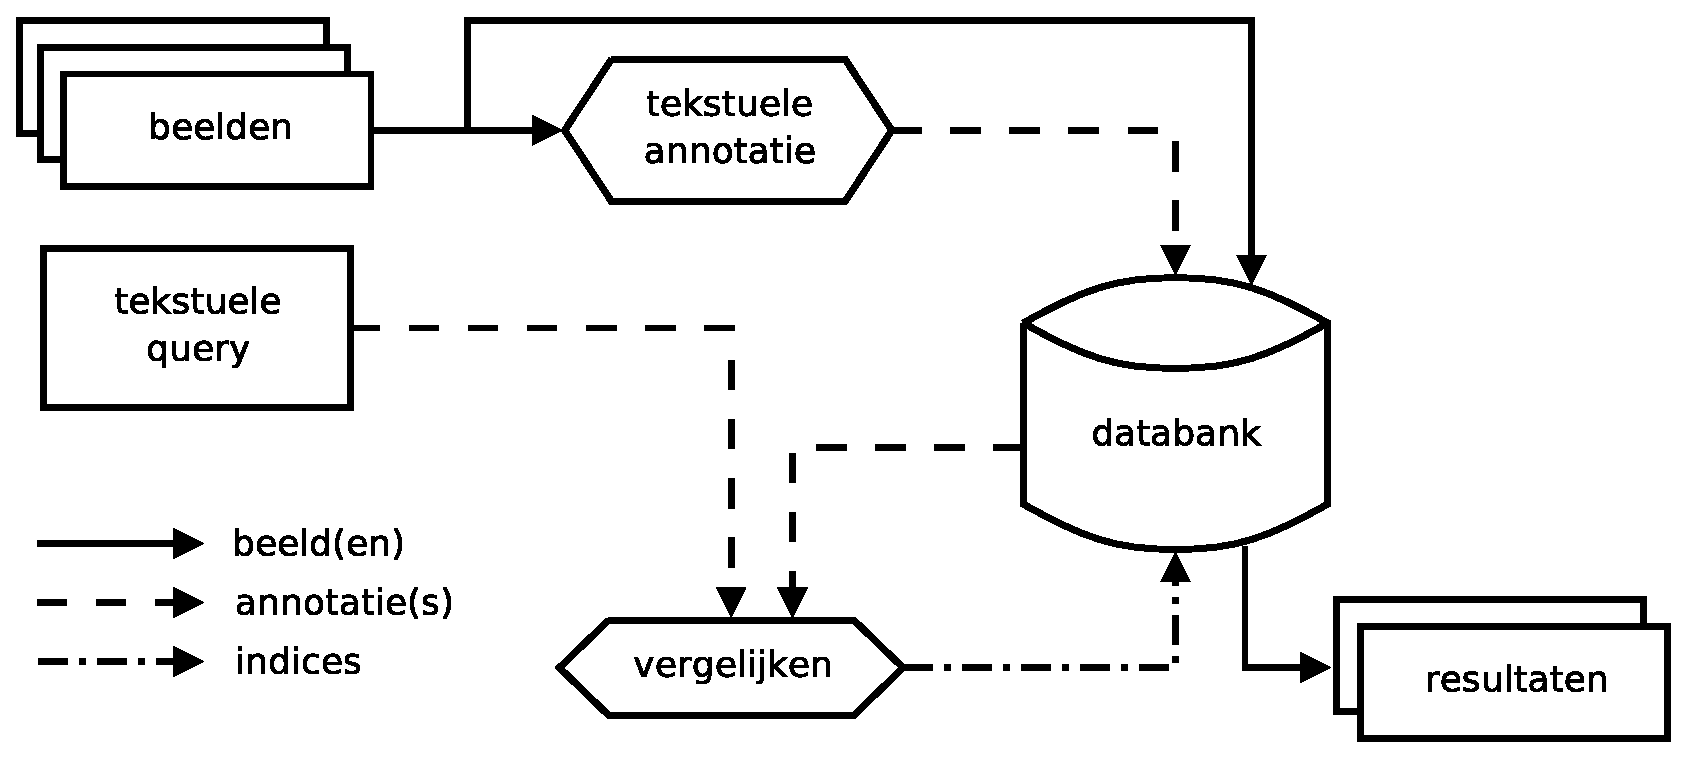
\includegraphics[width=9cm]{images/tbir.eps}
\label{fig:tbir}
}
\vspace{5pt}
\subfigure[]{
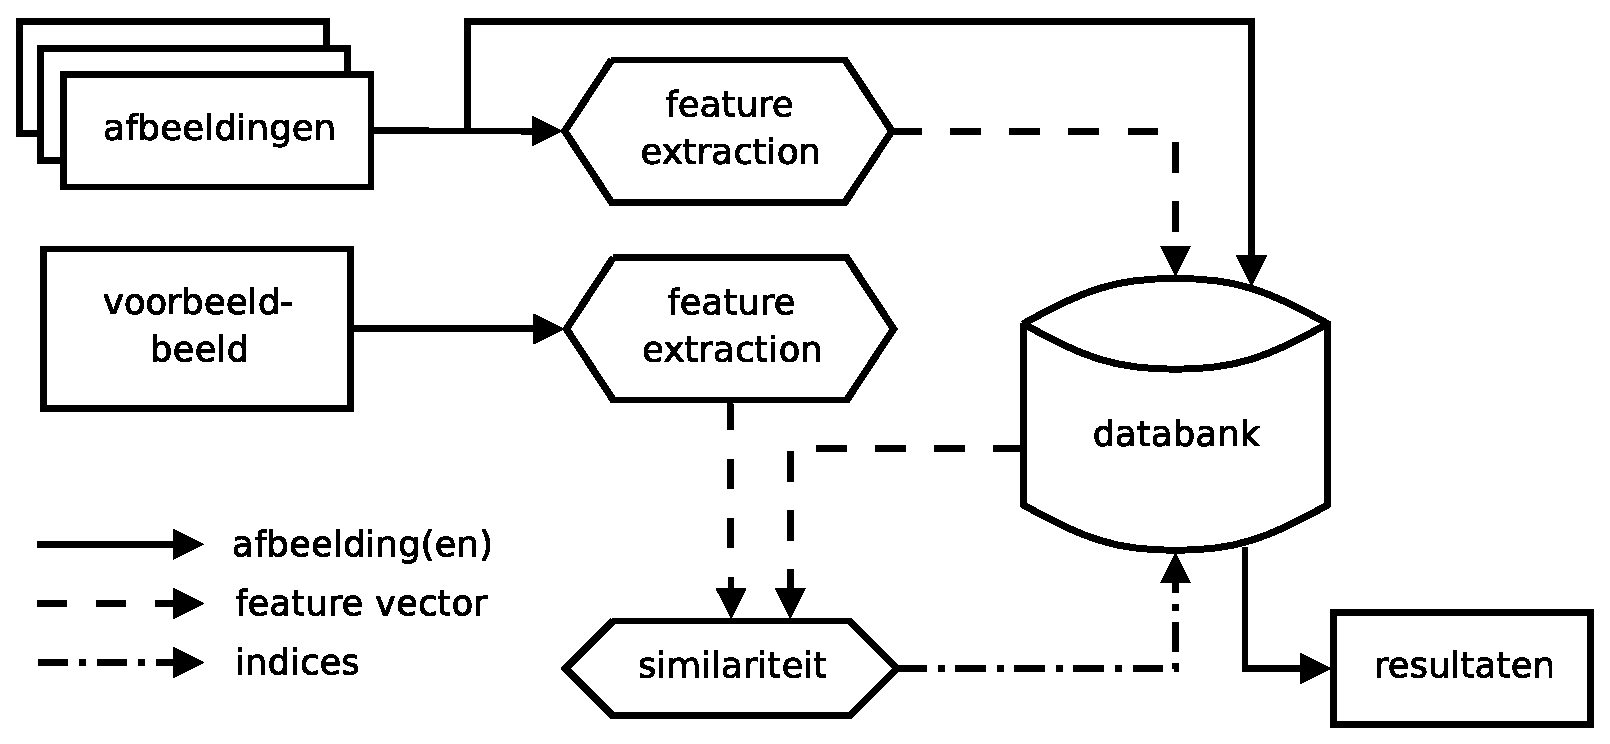
\includegraphics[width=9cm]{images/cbir.eps}
\label{fig:cbir}
}
\vspace{5pt}
\subfigure[]{
\includegraphics[width=9cm]{images/simgeb_rangschikken.eps}
\label{fig:simgeb_rangschikken}
}
\caption{\label{fig:cbir_en_tbir}Algemene architectuur van (a) een TBIR-systeem, 
(b) een CBIR-systeem en (c) een systeem dat het similariteitsgebaseerd rangschikking
van de zoekresultaten implementeert.}
\end{figure}

\section{Similariteitsgebaseerd rangschikken van de zoekresultaten}

Doordat CBIR-systemen zeer complex zijn, is het op dit moment nog niet mogelijk om ze te gebruiken voor het 
doorzoeken van zeer omvangrijke databanken. Bovendien beschikt de gebruiker niet altijd over
een geschikt voorbeeld. Dat probleem kan eventueel nog opgelost worden door gebruik
te maken van een voorbeeld-schets, maar ook dat is in de praktijk niet altijd even handig.
Het is bijgevolg zinvol om te zoeken naar manieren om inhoudgebaseerde aspecten toe te voegen aan
TBIR-systemen. 

De manier die we in deze scriptie bespreken, is het 
similariteitsgebaseerd rangschikken van de zoekresultaten van een TBIR-systeem. 
Figuur~\ref{fig:simgeb_rangschikken} toont de algemene architectuur van een systeem
dat die techniek implementeert. We verwachten
nog steeds dat de gebruiker een tekstuele query opgeeft, waarop het systeem antwoordt met een 
lijst van beelden die overeenkomen met die query. Daarna heeft de gebruiker echter ook nog 
de mogelijkheid om een verzameling van voorbeelden te kiezen uit die lijst. Het 
systeem zorgt er vervolgens voor dat de zoekresultaten gerangschikt worden in 
volgorde van similariteit met de voorbeelden.

Beschouw bijvoorbeeld de zoekresultaten uit figuur~\ref{fig:resultaten_orig_banaan}. Als
we effectief op zoek zijn naar een beeld van een banaan, dan zijn het
eerste en het voorlaatste beeld vrij goede resultaten. Bij een uitbreiding die het 
similariteitsgebaseerd rangschikken implementeert, kunnen die beelden als
voobeeld opgegeven worden. Via \'e\'en van de technieken die we verder in dit
eindwerk bespreken, bekomen we dan de rangschikking uit 
figuur~\ref{fig:resultaten_sorted_banaan}. Die rangschikking kan eventueel nog 
verder verfijnd worden door bijkomende voorbeelden op te geven.

\begin{figure}[!bp]
\vspace{10pt}
\centering
\begin{tabular}{@{}ccccc@{}}
\includegraphics[scale=0.6]{images/banaan_sorted_1_1.eps} &
\includegraphics[scale=0.6]{images/banaan_sorted_1_2.eps} &
\includegraphics[scale=0.6]{images/banaan_sorted_1_3.eps} &
\includegraphics[scale=0.6]{images/banaan_sorted_1_4.eps} &
\includegraphics[scale=0.6]{images/banaan_sorted_1_5.eps}\vspace{10pt}\\
\includegraphics[scale=0.6]{images/banaan_sorted_2_1.eps} &
\includegraphics[scale=0.6]{images/banaan_sorted_2_2.eps} &
\includegraphics[scale=0.6]{images/banaan_sorted_2_3.eps} &
\includegraphics[scale=0.6]{images/banaan_sorted_2_4.eps} &
\includegraphics[scale=0.6]{images/banaan_sorted_2_5.eps}\vspace{10pt}\\
\includegraphics[scale=0.6]{images/banaan_sorted_3_1.eps} &
\includegraphics[scale=0.6]{images/banaan_sorted_3_2.eps} &
\includegraphics[scale=0.6]{images/banaan_sorted_3_3.eps} &
\includegraphics[scale=0.6]{images/banaan_sorted_3_4.eps} &
\includegraphics[scale=0.6]{images/banaan_sorted_3_5.eps}\vspace{10pt}\\
\includegraphics[scale=0.6]{images/banaan_sorted_4_1.eps} &
\includegraphics[scale=0.6]{images/banaan_sorted_4_2.eps} &
\includegraphics[scale=0.6]{images/banaan_sorted_4_3.eps} &
\includegraphics[scale=0.6]{images/banaan_sorted_4_4.eps} &
\includegraphics[scale=0.6]{images/banaan_sorted_4_5.eps}\vspace{10pt}\\
\includegraphics[scale=0.6]{images/banaan_sorted_5_1.eps} &
\includegraphics[scale=0.6]{images/banaan_sorted_5_2.eps} &
\includegraphics[scale=0.6]{images/banaan_sorted_5_3.eps} &
\includegraphics[scale=0.8]{images/banaan_sorted_5_4.eps} &
\includegraphics[scale=0.6]{images/banaan_sorted_5_5.eps}
\end{tabular}
\vspace{10pt}
\caption{\label{fig:resultaten_sorted_banaan}De eerste 25 gerangschikte zoekresultaten voor de query "banaan".}
\end{figure}
\chapter{Wiskundige fundamenten}

In dit hoofdstuk introduceren we eerst enkele basisbegrippen uit de vaagverzamelingenleer. 
Daarna geven we een overzicht van de similariteitsmaten en aggregatieoperatoren waarvan
we in het vervolg van deze scriptie gebruik zullen maken.

\section{Vaagverzamelingen}

De collectie van alle mogelijke elementen noemen we het \emph{universum} (bijvoorbeeld de
natuurlijke getallen). Een verzameling bevat bepaalde elementen uit dit universum (bijvoorbeeld de 
verzameling van de priemgetallen). 

In het geval van een \emph{scherpe verzameling}, behoort elk 
element uit het universum wel of niet tot de verzameling. Andere mogelijkheden zijn er
niet. Een dergelijke verzameling kan bijgevolg 
gerepresenteerd worden door een \emph{karakteristieke afbeelding}, die elk element uit het 
universum afbeeldt op 0 of 1. Dit getal noemen we de \emph{lidmaatschapsgraad} van het element 
in kwestie. De klasse van scherpe verzamelingen in een universum $X$ stellen we voor door 
$\mathcal{P}(X)$.
\begin{definitie}
Zij $X$ een universum. De karakteristieke afbeelding $\mu_A$ van een scherpe verzameling $A$ in $X$
wordt gedefinieerd als de $X - \{0,1\}$ afbeelding:
$$
\begin{array}{lllll}
\mu_A: 	& X & \to 		& \{0,1\}	& \\
		& x & \mapsto 	& 1,		& \textrm{ als } x \in A \\
		& x & \mapsto 	& 0,		& \textrm{ als } x \notin A
\end{array}
$$
\end{definitie}

Bij een \emph{vaagverzameling} kunnen alle waarden tussen 0 en 1 als lidmaatschapsgraad 
voorkomen. De karakteristiek afbeelding is in dit geval dus een $X - [0,1]$ afbeelding:
\begin{definitie}
Zij $X$ een universum. Een vaagverzameling $A$ in $X$ wordt gekarakteriseerd door een $X - [0,1]$
afbeelding  $\mu_A$:
$$
\begin{array}{lllll}
\mu_A: 	& X & \to 		& [0,1]	& \\
		& x & \mapsto 	& \mu_A(x),		& \forall x \in A
\end{array}
$$
\end{definitie}
\noindent
Een element $x \in X$ behoort dus tot de vaagverzameling $A$ met lidmaatschapsgraad $\mu_A(x)$.
Voor de eenvoud zullen we in het vervolg $\mu_A(x)$ steeds noteren als $A(x)$. We zullen dus 
met andere woorden geen onderscheid meer maken tussen de vaagverzameling en de 
lidmaatschapsfunctie. Voor de klasse van vaagverzamelingen in een universum $X$ gebruiken we
de notatie $\mathcal{F}(X)$.

De \emph{drager} en de \emph{kern} van een vaagverzameling zijn twee belangrijke begrippen: 
\begin{definitie}
De drager van een vaagverzameling $A$ in $X$ wordt gedefinieerd als:
$$
supp\ A = \{x \in X \mid A(x) > 0\} 
$$
\end{definitie}
\begin{definitie}
De kern van een vaagverzameling $A$ in $X$ defini\"eren we als volgt:
$$
ker\ A = \{x \in X \mid A(x) = 1\}
$$
\end{definitie}
\noindent
Ook het begrip \emph{cardinaliteit} speelt vaak een belangrijke rol. De cardinaliteit van een 
een eindige scherpe verzameling wordt gegeven door het aantal elementen in die verzameling. 
Dit concept kan uitgebreid worden naar vaagverzamelingen door gebruik te maken van het begrip 
\emph{sigma count}:
\begin{definitie}
De sigma count van een vaagverzameling $A$ met eindige drager in een universum $X$ wordt
gedefinieerd door:
$$
|A|=\sum_{x \in X} A(x)
$$
\end{definitie}

\section{Bewerkingen op vaagverzamelingen}

We beginnen met het defini\"eren van de begrippen \emph{negator}, \emph{conjunctor} en 
\emph{disjunctor}. Deze operatoren zijn uitbreidingen van de klassieke logische operatoren
$\lnot$ (negatie), $\land$ (conjunctie) en $\lor$ (disjunctie).
\begin{definitie}
Een negator $\mathcal{N}$ op $[0,1]$ is een dalende $[0,1] - [0,1]$ afbeelding die voldoet
aan de randvoorwaarden $\mathcal{N}(0)=1$ en $\mathcal{N}(1)=0$. 
\end{definitie}
\begin{definitie}
Een conjunctor $\mathcal{C}$ op $[0,1]$ is een stijgende $[0,1]^2 - [0,1]$ afbeelding die voldoet aan de
randvoorwaarden $\mathcal{C}(0,0)=\mathcal{C}(0,1)=\mathcal{C}(1,0)=0$ en $\mathcal{C}(1,1)=1$.
\end{definitie}
\begin{definitie}
Een disjunctor $\mathcal{D}$ op $[0,1]$ is een stijgende $[0,1]^2 - [0,1]$ afbeelding die voldoet
aan de randvoorwaarden $\mathcal{D}(1,0)=\mathcal{D}(0,1)=\mathcal{D}(1,1)=1$ en 
$\mathcal{D}(0,0)=0$.
\end{definitie}

De meest gebruikte negator is de standaardnegator $N_S$. Het minimum $C_M$ en het algebra\"isch 
product $C_P$ zijn veelgebruikte conjunctors. Bij de disjunctors zijn het maximum $D_M$ en de
probabilistische som $D_P$ dan weer populaire mogelijkheden. Deze operatoren worden als 
volgt gedefinieerd:
$$
\begin{array}{r@{\quad=\quad}l}
N_S(x) & 1 - x \\
C_M(x,y) & min(x,y) \\
C_P(x,y) & x \cdot y \\
D_M(x,y) & max(x,y) \\
D_P(x,y) & x +y - x \cdot y,
\end{array}
$$
voor alle $(x,y)$ in $[0,1]^2$.

We kunnen de bovenstaande operatoren nu gebruiken om de klassieke verzameltechnische bewerkingen 
$co$ (complement), $\cap$ (doorsnede) en $\cup$ (unie) te
veralgemenen tot bewerkingen op vaagverzamelingen.
\begin{definitie}
Het $\mathcal{N}$-complement $co_\mathcal{N} A$ van een vaagverzameling $A$ in $X$ wordt gedefinieerd
door de volgende vaagverzameling in X:
$$
(co_\mathcal{N} A)(x) = \mathcal{N}(A(x)),
$$
voor alle $x$ in $X$, met $\mathcal{N}$ een negator.
\end{definitie}
\begin{definitie}
De $\mathcal{C}$-doorsnede $A \cap_\mathcal{C} B$ van twee vaagverzamelingen $A$ en $B$ in $X$
wordt gedefinieerd door de volgende vaagverzameling in $X$:
$$
(A \cap_\mathcal{C} B)(x) = \mathcal{C}(A(x),B(x)),
$$
voor alle $x$ in $X$, met $\mathcal{C}$ een conjunctor.
\end{definitie}
\begin{definitie}
De $\mathcal{D}$-unie $A \cup_\mathcal{D} B$ van twee vaagverzamelingen $A$ en $B$ in $X$ wordt gedefinieerd door de
volgende vaagverzameling in $X$:
$$
(A \cup_\mathcal{D} B)(x) = \mathcal{D}(A(x),B(x)),
$$
voor alle $x$ in $X$, met $\mathcal{D}$ een disjunctor.
\end{definitie}

In het vervolg van deze scriptie zullen we doorgaands 
$(\mathcal{N},\mathcal{C},\mathcal{D})=(N_S,C_M,D_M)$ kiezen. We voeren daarom de volgende
verkorte notaties in:
$$
\begin{array}{r@{\quad=\quad}l}
A^c 		& co_{N_S} A \\
A \cap B 	& A \cap_{C_M} B \\
A \cup B	& A \cup_{D_M} B,
\end{array}
$$
waarbij $A$ en $B$ vaagverzamelingen zijn.


\section{L-vaagverzamelingen}

\section{Aggregatieoperatoren} 
\chapter{Enkele begrippen uit beeldverwerking}

We zullen in het vervolg van deze scriptie ook gebruik maken van enkele
begrippen en technieken uit beeldverwerking. In dit hoofdstuk geven we 
een overzicht van die begrippen en beschrijven we kort de verwante
technieken.

\section{Modellering van kleuren en beelden}

\subsection{Kleurmodellen}

Een \emph{kleurmodel} is een abstract mathematisch model dat beschrijft hoe kleuren gerepresenteerd 
kunnen worden als $n$-tallen uit $\mathbb{R}^n$. RGB is het meest gebruikte kleurmodel. In dat model is elke kleur
een gewogen som van drie hoofdkleuren: rood, groen en blauw. De gewichten van die som
worden gebruikt als componenten van het drietal dat de kleur voorstelt. Figuur~\ref{fig:rgb}
toont de grafische voorstelling van het RGB-model.
%Naast RGB zijn ook
%HSV en L*a*b* populaire kleurmodellen \cite{philips:beeldverwerking}.

De kleuren die op basis van een bepaald model kunnen voorgesteld worden, vormen een \emph{kleurruimte}. 
In het geval van RGB is dat een driedimensionale ruimte. De kleuren in die ruimte zijn afhankelijk
van de manier waarop men ``rood'', ``groen'' en ``blauw'' definieert. Veelgebruikte kleurruimtes 
op basis van het RGB-model zijn sRGB en Adobe RGB.
Hoewel het strikt gezien niet correct is, wordt de term ``kleurruimte'' vaak ook voor het
kleurmodel gebruikt. Men heeft het dus dikwijls over \emph{de} RGB kleurruimte, terwijl er eigenlijk meerdere
kleurruimtes bestaan die gebaseerd zijn op RGB. 

\begin{figure}[tp]
\begin{center}
\subfigure[]{
\includegraphics[height=4cm]{images/rgb.eps}
\label{fig:rgb}
}
\qquad
\subfigure[]{
\includegraphics[height=4cm]{images/hsv.eps}
\label{fig:hsv}
}
\qquad
\subfigure[]{
\includegraphics[height=4cm]{images/lab.eps}
\label{fig:lab}
}
\caption{\label{fig:kleurmodellen}Grafische voorstelling van (a) het RGB-model, (b) het HSV-model en (c) het L*a*b*-model.}
\end{center}
\end{figure}

Ook in het HSV kleurmodel \cite{tkalcic:colour_spaces} wordt elke kleur voorgesteld 
door een drietal. Men noemt de componenten van zo'n drietal respectievelijk 
``hue'', ``saturation'' en ``value''. De eerste van die componenten 
correspondeert met de kleurtint, terwijl de overige componenten de saturatie
en de helderheid aangeven. Men kan een kleur $(r,g,b) \in [0,1]^3$ uit het RGB 
model als volgt omzetten naar een kleur $(h,s,v) \in [0,1]^3$ in het HSV-model: 
\begin{align*}
h' & = \begin{cases}
60 \cdot \frac{g - b}{\max \{r,g,b\} - \min \{r,g,b\}} & \textrm{als } \max \{r,g,b\} = r \\[2pt]
60 \cdot \frac{b - r}{\max \{r,g,b\} - \min \{r,g,b\}} + 120 & \textrm{als } \max \{r,g,b\} = g \\[2pt]
60 \cdot \frac{r - g}{\max \{r,g,b\} - \min \{r,g,b\}} + 240 & \textrm{als } \max \{r,g,b\} = b
\end{cases} \\[2pt]
h & = \begin{cases}
\frac{h' \bmod 360}{360} & \textrm{als } h' \bmod 360 \geq 0 \\[2pt] 
\frac{360 - (h' \bmod 360)}{360} & \textrm{als } h' \bmod 360 < 0 
\end{cases} \\[2pt]
s & = \frac{\max \{r,g,b\} - \min \{r,g,b\}}{\max \{r,g,b\}} \\ %[6pt] 
v & = \max \{r,g,b\}
\end{align*}
Als $s=0$ dan is $h$ niet gedefinieerd. Dat is logisch vermits we dan te 
maken hebben met een grijswaarde. Indien $v=0$ dan zijn $s$ en $h$ niet gedefinieerd. We 
hebben het in dat geval dan ook over puur zwart, waarvoor er geen kleurtint of 
saturatie kan gespecificeerd worden. In de praktische implementatie geven we 
niet gedefinieerde componenten de waarde $0$. Uit figuur~\ref{fig:hsv} blijkt dat
het HSV-model de vorm van een kegel heeft.

Een kleur in het Irb-model bestaat uit een intensiteit en een genormaliseerde $r$ en $b$ 
\cite{ohta:color_info_for_region_segm}:
\begin{displaymath}
 i = \frac{r+g+b}{3} \qquad r' = 
\frac{r}{r+g+b} \qquad b' = \frac{b}{r+g+b}
\end{displaymath}
met $r,g,b \in [0,1]$ de co\"ordinaten van de beschouwde kleur in het RGB-model. 

Het I1I2I3-model, dat werd voorgesteld door Ohta 
\cite{ohta:color_info_for_region_segm}, is een \emph{opponent color space}. 
We zetten een kleur $(r,g,b) \in 
[0,1]^3$ uit het RGB-model als volgt om:
\begin{displaymath}
%\begin{array}{rcl}
i_1 = \frac{r+g+b}{3} \qquad i_2 = \frac{r-b}{2} \qquad i_3 = \frac{2 \cdot g - 
r - b}{4}
%\end{array}
\end{displaymath}
De eerste component is achromatisch (\emph{white-black}), terwijl de overige 
twee chromatisch zijn (\emph{red-green} en \emph{yellow-blue}).
We gebruiken hier, zoals in \cite{wang:cbir_using_daubechies_wavelets}, een 
genormaliseerde vorm van dit model:
\begin{displaymath}
%\begin{array}{rcl}
c_1 = \frac{r+g+b}{3} \qquad c_2 = \frac{r + (1 - b)}{2} \qquad c_3 = \frac{r + 
2 \cdot (1 - g) + b}{4}
%\end{array}
\end{displaymath}

In het XYZ-model wordt een kleur voorgesteld door de volgende drie componenten: 
\begin{align*}
x & = 0.4124 \cdot r + 0.3576 \cdot g + 0.1805 \cdot b \\
y & = 0.2126 \cdot r + 0.7152 \cdot g + 0.0722 \cdot b \\
z & = 0.0193 \cdot r + 0.1192 \cdot g + 0.9505 \cdot b
\end{align*}
met $(r,g,b) \in [0,1]^3$ de vector van de kleur in het RGB-model. Hierbij 
is $y$ evenredig met de luminantie van de kleur in kwestie. 

De eerste component van een kleur in het Yxy-model is gelijk aan de $y$ 
component van die kleur in het XYZ-model. De overige twee componenten berekenen 
we als volgt:
\begin{displaymath}
x' = \frac{x}{x+y+z} \qquad y' = \frac{y}{x+y+z}
\end{displaymath}

In figuur~\ref{fig:lab} wordt de grafische voorstelling van het L*a*b*-model weergegeven. 
Een kleurruimte op basis van dat model is \emph{perceptueel uniform} 
\cite{sharma:digital_color_imaging}. Dat wil zeggen dat, in een dergelijke 
ruimte, de Euclidische afstand een goede maat is voor het waargenomen verschil 
tussen twee kleuren. De co\"ordinaten $(l,a,b)$ van een kleur in het 
L*a*b*-model kunnen als volgt benaderd worden
\cite{debaets:similariteitsmaten_voor_kleurbeelden, philips:beeldverwerking}:
\begin{align*}
l & = 116 \cdot f({\scriptstyle\frac{100 \cdot y}{255 \cdot y_0}}) - 16 \\[2pt] 
a & = 500 \cdot \left(f({\scriptstyle\frac{\scriptstyle 100 \cdot x}{\scriptstyle 255 \cdot x_0}}) - f({\scriptstyle\frac{\scriptstyle 100 \cdot y}{\scriptstyle 255 \cdot y_0}})\right) \\[2pt] 
b & = 200 \cdot \left(f({\scriptstyle\frac{\scriptstyle 100 \cdot y}{\scriptstyle 255 \cdot y_0}}) - f({\scriptstyle\frac{\scriptstyle 100 \cdot z}{\scriptstyle 255 \cdot z_0}})\right)
\end{align*}
met
\begin{displaymath}
f(t) = \begin{cases} 
t^\frac{1}{3} & \textrm{als } t > 0.008856 \\ 
7.787 \cdot t + \frac{16}{116} & \textrm{anders}
\end{cases}
\end{displaymath}
voor elke re\"ele $t$. Hierbij zijn $x_0$, $y_0$ en $z_0$ de
XYZ-co\"ordinaten van een wit referentiepunt. We gebruiken hier 
$255 \cdot (x_0,y_0,z_0)=(95.05,100,108.9)$.
We kunnen dan als volgt normaliseren:
\begin{displaymath}
l' = \frac{l}{100} \qquad a' = \frac{120 + 
\max\{\min\{a,120\},-120\}}{240} \qquad b' = \frac{120 + \max\{\min\{b,120\},-120\}}{240}
\end{displaymath}


\subsection{Kleurbeelden}

In een \emph{kleurbeeld} heeft elk beeldpunt een bepaalde kleur, die beschreven wordt met
behulp van een kleurmodel. Met andere woorden: de kleur van een beeldpunt wordt voorgesteld 
als een $n$-tal uit
$\mathbb{R}^n$. Zoals hierboven reeds een aantal keer werd ge\"illustreerd, kunnen dergelijke 
$n$-tallen genormaliseerd worden tot $n$-tallen uit $[0,1]^n$. We kunnen een $m$-dimensionaal 
kleurbeeld dus modelleren als een $\mathbb{R}^m - [0,1]^n$ afbeelding $b$. 
In de praktijk wordt een beeld echter voorgesteld als een rooster bestaande uit een
eindig aantal beeldpunten. Bijgevolg zal $b$ eerder een afbeelding van een deelverzameling van 
$\mathbb{N}^2$ naar $[0,1]^n$ zijn. 

Om geen rekening te moeten houden met ``randgevallen'', beschouwen voor elk beeld $b$ ook een
met nullen uitgebreide versie $\mathring{b}$. Voor een beeld $b$ van $M$ bij $N$ beeldpunten
defini\"eren we de $\mathbb{Z}^2 - [0,1]^n$ afbeelding $\mathring{b}$ als volgt:
\begin{displaymath}
\mathring{b}(x,y) = \begin{cases}
b(x,y) & \textrm{als } 0 \le x < M \textrm{ en } 0 \le y < N \\
(0,0,\ldots,0) & \textrm{anders}
\end{cases}
\end{displaymath}

\section{Kleurkwantisatie}
\label{sectie:kleurkwantisatie}

Een kleurruimte bevat meestal een groot aantal 
kleuren. Zo gebruikt men voor een RGB-ruimte bijvoorbeeld typisch 8 bits per 
kleurcomponent. Dit geeft een totaal van 24 bits per kleur, zodat men dus 
$2^{24}=2^4 \cdot 2^{20}=16 \cdot 2^{20} \approx 16 \cdot 10^6$ kleuren kan 
voorstellen.

Om de complexiteit te beperken, kan het dus nodig zijn om het aantal kleuren te 
reduceren. Dat kan door middel van \emph{kleurkwantisatie}. Daarbij groeperen we de kleuren in 
zogenaamde \emph{bins}. We beschouwen dus geen aparte kleuren meer, maar wel 
verzamelingen van kleuren. De kleuren die in dezelfde bin zitten, worden dan 
vervangen door \'e\'en enkele kleur. Het \emph{kleurenpalet} is de verzameling 
van alle bin-kleuren. Bij eenvoudige kwantisatietechnieken wordt steeds 
hetzelfde palet gebruikt, onafhankelijk van de voor te stellen beelden. Meer 
geavanceerde technieken proberen een palet te gebruiken dat optimaal is voor de 
beschouwde beelden.

Wiskundig kunnen we kleurkwantisatie modelleren aan de hand van twee functies: 
$bin$ en $col$. De eerste functie associeert met elke kleur $c$, uit de 
kleurruimte $C$, het nummer van de corresponderende bin. Met behulp van de 
tweede functie kan men dan de kleur van die bin bepalen.

\subsection{Uniforme kwantisatie}

Bij \emph{uniforme kwantisatie} wordt elke kleurcomponent uniform verdeeld in een 
aantal intervallen. Als we zorgen dat $C=[0,1]^l$, $l > 0$, dan kunnen we de 
volgende definitie voor $bin$ gebruiken:
\begin{displaymath}
\begin{array}{lrcll}
bin: & C & \to & \{1,2,...,N\}\\[5pt] & (c_1,c_2,\ldots,c_l) & \mapsto & \left[ 
\displaystyle\sum_{i=1}^l \left( \prod_{j=1}^{i-1} N_j \right) \mathit{fl}(c_i, N_i) \right] 
+ 1, & \forall (c_1,c_2,\ldots,c_l) \in C
\end{array}
\end{displaymath}
met $N_j$ het aantal bins voor de $j$-de component, $N$ het totale aantal 
bins ($N=N_1 \cdot N_2 \cdot \ldots \cdot N_l$) en 
\begin{displaymath}
\mathit{fl}(x,n) = \begin{cases}
\lfloor x \cdot n \rfloor & \textrm{als } x < 1 \\ 
n - 1 & \textrm{als } x = 1
\end{cases}
\end{displaymath}
voor alle $x \in [0,1]$ en $n \in \mathbb{N}$. De middelste waarden van de 
intervallen doen hierbij dienst als componenten van de kleur van een bin:
\begin{displaymath}
\begin{array}{lrcll}
col: & \{1,2,\ldots,N\} & \to & C \\ & n & \mapsto & (col_1(n), col_2(n), 
\dots, col_l(n)), & \forall n \in \{1,2,\ldots,N\}
\end{array}
\end{displaymath}
waarbij 
\begin{displaymath}
col_i(n) = \frac{n}{\prod_{j=1}^i N_j} + \frac{1}{2 \cdot N_i}
\end{displaymath} 
voor alle $n \in \{1,2,\ldots,N\}$ en $i \in \{1,2,\ldots,l\}$.

Bij image retrieval is doorgaans vooral de kleurtint op zich belangrijk. Door
minder belang te hechten aan de luminantie kan de prestatie zelfs verbeteren,
vermits de similariteitsmaten dan bijvoorbeeld minder afhankelijk zijn van
belichtingsvariaties. 

Een mogelijke manier om uniform te kwantiseren is dus
het HSV-model gebruiken en meer belang hechten aan de eerste kleurcomponent. 
Dat doen we door $N_1=16$, $N_2=4$ en $N_3=4$ te kiezen.
%Bovendien is het discriminerend
%vermogen van dit histogram waarschijnlijk ook beter dan dat van een ongecomprimeerd kleurhistogram.
Die keuzes voor $N_1$, $N_2$ en $N_3$ stemmen overeen met de keuzes die men 
gemaakt heeft voor de \emph{scalable color descriptor} (SCD), die gedefinieerd 
wordt in de MPEG-7 standaard \cite{manjunath:color_and_texture_descriptors}.

Via analoge redeneringen voor de andere kleurmodellen, bekomen we de zes manieren 
uit tabel~\ref{tab:uniforme_kwantisatie} om uniform te kwantiseren met een vast kleurenpalet.
Elk van die manieren gebruikt $256$ bins.

\begin{table}[tbp]
\begin{center}
\begin{tabular}{|c|cccccc|}
\hline
 		& HSV & Irb & I1I2I3 & XYZ & Yxy & L*a*b* \\
\hline
$N_1$ 	& 16 & 4 & 4 & 8 & 4 & 4 \\
$N_2$	& 4  & 8 & 8 & 4 & 8 & 8 \\
$N_3$	& 4  & 8 & 8 & 8 & 8 & 8 \\
\hline
\end{tabular}
\caption{\label{tab:uniforme_kwantisatie}Zes manieren om uniform te kwantiseren met een vast kleurenpalet.}
\end{center}
\end{table}


\subsection{Niet-uniforme kwantisatie}

We hebben reeds vermeld dat bij image retrieval vooral de tinten van de kleuren belangrijk zijn. Daarom 
lijkt het op het eerste zicht geen slecht idee om kleuren met een zelfde kleurtint te groeperen in 
\'e\'en enkele bin. De eerste HSV-component bepaalt dan tot welke bin een kleur behoort. We passen
met andere woorden uniforme HSV-kwantisatie toe met $(N_1,N_2,N_3)=(256,1,1)$. Een probleem daarbij 
is echter dat beelden ook grijswaarden kunnen bevatten. Voor grijswaarden is de ``hue''-component immers 
niet gedefinieerd. De waarde 0 gebruiken voor niet-gedefinieerde kleurtinten lost dit probleem maar 
gedeeltelijk op, want dan komen alle grijswaarden in dezelfde bin terecht. Dat kan wel vermeden worden 
door bijvoorbeeld $(N_1,N_2,N_3)=(64,1,4)$ te kiezen, maar dan kunnen we maar 64 tinten meer onderscheiden.

Met behulp van niet-uniforme kwantisatie komen we tot een betere oplossing. Als we het HSV-model van naderbij
bekijken, dan merken we dat elke kleur getransformeerd kan worden in een grijstint door de saturatie
voldoende te verlagen. De waarde van de saturatie waarbij die transformatie plaatsvindt, hangt af
van de helderheid. We gaan daarom als volgt te werk. Als $s > 1 - 0.8 \cdot v$ dan benaderen we de kleur
met de kleurtint en kwantiseren we uniform met $(N_1,N_2,N_3)=(240,1,1)$. In het andere geval hebben we
te maken met een grijstint en kwantiseren we uniform met $(N_1,N_2,N_3)=(1,1,16)$. We combineren dus
twee uniforme kwantisaties tot \'e\'en niet-uniforme. Vermits $240 + 16 = 256$
slagen we er zo in om 240 kleurtinten te onderscheiden, zonder het aantal bins te verhogen. Omdat het
``Perceptually Smooth Color Transition Histogram'' uit \cite{sural:perceptually_smooth_histogram} 
gebaseerd is op deze kwantisatietechniek, spreken we van Smooth Color Transition (SCT) kwantisatie.  

Een andere niet-uniforme manier om te kwantiseren, is het mappen van de kleuren op elf 
\emph{focale kleuren} \cite{van_den_broek:human_color_categorization_for_cbir}: zwart, wit, rood, groen, geen, blauw, bruin, paars, roze, oranje en grijs.
Experimenten hebben aangetoond dat de mens geneigd is om enkel die kleurcategorie\"en te gebruiken bij 
het beredeneren, onthouden en waarnemen van kleuren. We kunnen voor elke kleur de juiste mapping bepalen
door op zoek te gaan naar de focale kleur die in het L*a*b*-model het dichtst bij die gegeven kleur ligt.

\emph{Neural Image Quantization} (NeuQuant) \cite{dekker:neuquant} en de \emph{Wu quantizer} 
\cite{wu:color_quantization_by_dynamic_programming_and_principal_analysis} zijn twee
populaire kwantisatietechnieken die, in tegenstelling tot de technieken die we 
tot nu toe bekeken hebben, een variabel kleurenpalet gebruiken. De eerste techniek gebruikt een
zogenaamd \emph{Kohonen neuraal netwerk} om clusters van kleuren te vormen. Vervolgens worden 
alle kleuren uit een cluster dan naar dezelfde kleur gekwantiseerd. Bij de tweede techniek 
wordt er gebruik gemaakt van \emph{dynamisch programmeren} en van een statistische techniek voor 
het reduceren van de dimensionaliteit van data, 
die \emph{principal component analysis} (PCA) genoemd wordt. 
NeuQuant geeft doorgaans iets betere resultaten, maar Wu's techniek is
sneller. Uit figuur~\ref{fig:rekentijden_quant} blijkt echter dat het verschil in rekentijd zich
enkel manifesteert als er naar een relatief groot aantal kleuren gekwantiseerd wordt. Voor een
klein aantal kleuren is NeuQuant zelfs iets sneller. Anderzijds is Wu's techniek wel meer
geschikt voor kwantisatie naar een zeer klein aantal kleuren.
 

\begin{figure}[tbp]
\begin{center}
\subfigure[]{
\begin{minipage}[t]{0.4\textwidth}
\vspace{0pt}
\centering
\includegraphics[height=3.8cm]{plots/uniform_quant_small_filled.eps}
\end{minipage}
\begin{minipage}[t]{0.4\textwidth}
\vspace{0pt}
\centering
\includegraphics[height=4.1cm]{plots/neuquant_vs_wu_small_filled.eps}
\end{minipage}
\label{fig:rekentijden_quant_small}
}
\subfigure[]{
\begin{minipage}[t]{0.4\textwidth}
\vspace{0pt}
\centering
\includegraphics[height=3.8cm]{plots/uniform_quant_big_filled.eps}
\end{minipage}
\begin{minipage}[t]{0.4\textwidth}
\vspace{0pt}
\centering
\includegraphics[height=4.1cm]{plots/neuquant_vs_wu_big_filled.eps}
\end{minipage}
\label{fig:rekentijden_quant_big}
}
\caption{\label{fig:rekentijden_quant}Vergelijking van de rekentijden bij kwantisatie van (a) een klein en (b) een groot beeld.}
\end{center}
\end{figure}

\subsection{Enkele voorbeelden}

We illustreren de bovenstaande technieken door ze toe te passen op de beelden uit 
figuur~\ref{fig:kwantistatie_originelen}. De eerste twee van die beelden hebben we geconstueerd
door in het HSV-model twee componenten te laten vari\"eren en \'e\'en component constant te houden.
Bij figuur~\ref{fig:hsv_constant_s} is de saturatie steeds gelijk aan $1$ en hebben we de kleurtint 
horizontaal en de helderheid vertikaal laten vari\"eren. Figuur~\ref{fig:hsv_constant_v} werd 
op een analoge manier geconstrueerd, maar in dit geval is de helderheid constant.
De beelden die we bekomen door toepassing van de zes manieren om uniform te kwantiseren,
worden weergegeven in figuur~\ref{fig:kwantistatie_uniform}. Figuur~\ref{fig:kwantistatie_niet-uniform}
toont de resultaten van de vier niet-uniforme kwantistatietechnieken.

\begin{figure}[tbp]
\begin{center}
\subfigure[]{
\includegraphics[height=2.8cm]{images/hsv_constant_s.eps}
\label{fig:hsv_constant_s}
}
\subfigure[]{
\includegraphics[height=2.8cm]{images/hsv_constant_v.eps}
\label{fig:hsv_constant_v}
}
\subfigure[]{
\includegraphics[height=2.8cm]{images/flowers.eps}
\label{fig:flowers}
}
\subfigure[]{
\includegraphics[height=2.8cm]{images/autumn.eps}
\label{fig:autumn}
}
\caption{\label{fig:kwantistatie_originelen}De beelden waarvan we de kleuren gaan kwantiseren op een aantal verschillende manieren.}
\end{center}
\end{figure}

\begin{figure}[tbp]
\begin{center}
\subfigure[]{
\includegraphics[height=2.8cm]{images/uniform_hsv_constant_s.eps}
\includegraphics[height=2.8cm]{images/uniform_hsv_constant_v.eps}
\includegraphics[height=2.8cm]{images/uniform_hsv_flowers.eps}
\includegraphics[height=2.8cm]{images/uniform_hsv_autumn.eps}
\label{fig:uniform_hsv}
}
\subfigure[]{
\includegraphics[height=2.8cm]{images/uniform_irb_constant_s.eps}
\includegraphics[height=2.8cm]{images/uniform_irb_constant_v.eps}
\includegraphics[height=2.8cm]{images/uniform_irb_flowers.eps}
\includegraphics[height=2.8cm]{images/uniform_irb_autumn.eps}
\label{fig:uniform_irb}
}
\subfigure[]{
\includegraphics[height=2.8cm]{images/uniform_i1i2i3_constant_s.eps}
\includegraphics[height=2.8cm]{images/uniform_i1i2i3_constant_v.eps}
\includegraphics[height=2.8cm]{images/uniform_i1i2i3_flowers.eps}
\includegraphics[height=2.8cm]{images/uniform_i1i2i3_autumn.eps}
\label{fig:uniform_i1i2i3}
}
\subfigure[]{
\includegraphics[height=2.8cm]{images/uniform_xyz_constant_s.eps}
\includegraphics[height=2.8cm]{images/uniform_xyz_constant_v.eps}
\includegraphics[height=2.8cm]{images/uniform_xyz_flowers.eps}
\includegraphics[height=2.8cm]{images/uniform_xyz_autumn.eps}
\label{fig:uniform_xyz}
}
\subfigure[]{
\includegraphics[height=2.8cm]{images/uniform_yxy_constant_s.eps}
\includegraphics[height=2.8cm]{images/uniform_yxy_constant_v.eps}
\includegraphics[height=2.8cm]{images/uniform_yxy_flowers.eps}
\includegraphics[height=2.8cm]{images/uniform_yxy_autumn.eps}
\label{fig:uniform_yxy}
}
\subfigure[]{
\includegraphics[height=2.8cm]{images/uniform_lab_constant_s.eps}
\includegraphics[height=2.8cm]{images/uniform_lab_constant_v.eps}
\includegraphics[height=2.8cm]{images/uniform_lab_flowers.eps}
\includegraphics[height=2.8cm]{images/uniform_lab_autumn.eps}
\label{fig:uniform_lab}
}
\caption{\label{fig:kwantistatie_uniform}De resultaten na uniforme kwantisatie op basis van (a) HSV, (b) Irb, (c) I1I2I3, (d) XYZ, (e) Yxy en (f) L*a*b*.}
\end{center}
\end{figure}

\begin{figure}[tbp]
\begin{center}
\subfigure[]{
\includegraphics[height=2.8cm]{images/sct_constant_s.eps}
\includegraphics[height=2.8cm]{images/sct_constant_v.eps}
\includegraphics[height=2.8cm]{images/sct_flowers.eps}
\includegraphics[height=2.8cm]{images/sct_autumn.eps}
\label{fig:sct}
}
\subfigure[]{
\includegraphics[height=2.8cm]{images/focal_constant_s.eps}
\includegraphics[height=2.8cm]{images/focal_constant_v.eps}
\includegraphics[height=2.8cm]{images/focal_flowers.eps}
\includegraphics[height=2.8cm]{images/focal_autumn.eps}
\label{fig:focal}
}
\subfigure[]{
\includegraphics[height=2.8cm]{images/neuquant_constant_s.eps}
\includegraphics[height=2.8cm]{images/neuquant_constant_v.eps}
\includegraphics[height=2.8cm]{images/neuquant_flowers.eps}
\includegraphics[height=2.8cm]{images/neuquant_autumn.eps}
\label{fig:neuquant}
}
\subfigure[]{
\includegraphics[height=2.8cm]{images/wu_constant_s.eps}
\includegraphics[height=2.8cm]{images/wu_constant_v.eps}
\includegraphics[height=2.8cm]{images/wu_flowers.eps}
\includegraphics[height=2.8cm]{images/wu_autumn.eps}
\label{fig:wu}
}
\caption{\label{fig:kwantistatie_niet-uniform}De resultaten na niet-uniforme kwantisatie op basis van (a) SCT, (b) focale kleuren, (c) NeuQuant en (d) de Wu quantizer.}
\end{center}
\end{figure}

\begin{figure}[tbp]
\begin{center}
\subfigure[]{
\includegraphics[height=2.8cm]{images/neuquant_constant_s_8.eps}
\includegraphics[height=2.8cm]{images/neuquant_constant_v_8.eps}
\includegraphics[height=2.8cm]{images/neuquant_flowers_8.eps}
\includegraphics[height=2.8cm]{images/neuquant_autumn_8.eps}
\label{fig:neuquant_8}
}
\subfigure[]{
\includegraphics[height=2.8cm]{images/wu_constant_s_8.eps}
\includegraphics[height=2.8cm]{images/wu_constant_v_8.eps}
\includegraphics[height=2.8cm]{images/wu_flowers_8.eps}
\includegraphics[height=2.8cm]{images/wu_autumn_8.eps}
\label{fig:wu_8}
}
\caption{\label{fig:kwantistatie_klein_aantal_kleuren}De resultaten na kwantisatie naar slechts 8 kleuren op basis van (a) NeuQuant en (b) de Wu quantizer.}
\end{center}
\end{figure}

De technieken met een variabel kleurenpalet doen het duidelijk beter dan diegene met een vast palet. 
In figuur~\ref{fig:rekentijden_quant} merken we echter dat kwantisatie met een vast kleurenpalet 
vaak een stuk sneller is. Zo gaat het uniform kwantiseren op basis van Irb bijvoorbeeld
twee keer zo snel als Wu kwantisatie naar hetzelfde aantal kleuren. Bovendien is het soms niet
gewenst dat voor alle beelden een andere verzameling van kleuren gebruikt wordt. In deze scriptie gebruiken
we kwantisatie trouwens louter om meer performante similariteitsmaten te constueren. De visuele kwaliteit
van de gekwantiseerde beelden is daarbij minder belangrijk. Similariteitsmaten op basis van kwantisatietechnieken 
waarbij de gekwantiseerde beelden een lagere kwaliteit hebben, presteren immers niet noodzakelijk
slechter dan maten die gebaseerd zijn op ``betere'' kwantisatietechnieken. Zo zouden we bijvoorbeeld 
betere kwantisatie kunnen bekomen door extra luminantiedata te behouden, maar daardoor zullen
de similariteitsmaten doorgaans minder goed werken vermits ze dan gevoeliger worden voor 
belichtingsvariaties.
%kunnen in bepaalde gevallen immers beter 
%presteren dan maten die gebaseerd zijn op ``betere'' kwantisatietechnieken.

Merk ook op dat uit figuur~\ref{fig:kwantistatie_klein_aantal_kleuren} inderdaad blijkt
dat NeuQuant minder geschikt is voor kwantisatie naar een zeer klein
aantal kleuren dan Wu's techniek. 

\section{Lineaire filters}
\label{sectie:lineaire_filters}

Bij het \emph{filteren} van een 2-dimensionaal beeld $b$ wordt de waarde $b(x,y)$ van een 
beeldpunt $(x,y) \in \mathbb{N}^2$ vervangen door een nieuwe waarde die afhangt van $b(x,y)$ 
en van de waarden van naburige beeldpunten. In het geval van een \emph{lineair filter} is die nieuwe waarde een lineaire combinatie 
van de oude waarden. Het beeld $b'$ dat we bekomen door $b$ lineair te filteren, wordt gegeven door
de volgende correlatie \cite{philips:beeldverwerking}:
\begin{displaymath}
b'(x,y) = \sum_{(k,l) \in \Omega_m} \mathring{b}(x+k,y+l) \cdot m(k,l)
\end{displaymath}
met $\mathring{b}$ de nuluitbreiding van $b$, $m$ een $\mathbb{N}^2 - \mathbb{R}$ afbeelding 
en $\Omega_m = \{ (k,l) \in \mathbb{N}^2 \mid m(k,l) \ne 0 \}$. 
De functie $m$ wordt het \emph{filtermasker} genoemd.

Het \emph{3x3 binomiaalfilter} is een voorbeeld van een lineair filter. Voor het filtermasker 
$m_{bin}$ van dat filter geldt $m_{bin}(-1,-1)=m_{bin}(-1,1)=m_{bin}(1,-1)=m_{bin}(1,1)=1/16$, 
$m_{bin}(-1,0)=m_{bin}(0,-1)=m_{bin}(1,0)=m_{bin}(0,1)=1/8$, $m_{bin}(0,0)=1/4$ en 
$m_{bin}(k,l)=0$ voor de overige $(k,l)$. Als we veronderstellen dat $m_{bin}(k,l)=0$ voor de 
posities $(k,l)$ die niet weergegeven worden, dan kunnen we dat masker noteren als een matrix:
\begin{displaymath}
\frac{1}{16}\left[ \begin{array}{ccc} 1 & 2 & 1\\ 2 & 4 & 2\\ 1 & 2 & 1 \end{array} \right]
= \frac{1}{16}\left[ \begin{array}{c} 1\\ 2\\ 1 \end{array} \right] \cdot 
\left[ \begin{array}{ccc} 1 & 2 & 1 \end{array} \right]
\end{displaymath}
Zoals ge\"illustreerd in figuur~\ref{fig:indische_ruizig_en_binom}, kan een binomiaalfilter gebruikt worden om ruis te onderdrukken.

\begin{figure}[tb]
\begin{center}
\subfigure[]{
\includegraphics[width=0.3\textwidth]{images/indische_ruizig.eps}
\label{fig:indische_ruizig}
}
\hspace{1cm}
\subfigure[]{
\includegraphics[width=0.3\textwidth]{images/indische_binom.eps}
\label{fig:indische_binom}
}
\caption{\label{fig:indische_ruizig_en_binom}Een ruizig beeld (a) en het resultaat na filteren met een binomiaalfilter (b).}
\end{center}
\end{figure}

\section{Eenvoudige randdetectie}
\label{sectie:randdetectie}

Beeldranden in een 2-dimensionaal beeld $b$ zijn plaatsen waar de luminantiecomponent $lum(x,y)$ van $b(x,y)$ 
sterk varieert als functie van $x$ en/of $y$. Op die plaatsen zullen de partieel afgeleiden $D_1 lum(x,y)$ en 
$D_2 lum(x,y)$ dus groot zijn. Bijgevolg zal de \emph{gradi\"ent} $\nabla lum$ daar ook groot zijn. We kunnen 
dus de volgende formule gebruiken om randen te detecteren in $b$: 
\begin{displaymath}
|\nabla lum(x,y)| / \sqrt{2} = \sqrt{(D_1 lum(x,y))^2 + (D_2 lum(x,y))^2} / \sqrt{2}
\end{displaymath}
met $lum$ de $\mathbb{N}^2 - [0,1]$ functie die met elk beeldpunt $(x,y)$ de juiste luminantiecomponent associeert.

Doordat $lum$ in de praktijk geen continue maar een discrete functie is, moeten we de partieel afgeleiden benaderen.
De Taylorreeksontwikkeling van een $\mathbb{R} - \mathbb{R}$ functie $f$ rond $x$ geeft
\begin{displaymath}
f(x+h) = f(x) + h D f(x) + \frac{h^2}{2!} D^2 f(x) + \ldots
\end{displaymath}
en ook
\begin{displaymath}
f(x-h) = f(x) - h D f(x) + \frac{h^2}{2!} D^2 f(x) + \ldots
\end{displaymath}
zodat
\begin{displaymath}
\frac{f(x+h) - f(x-h)}{2h} \approx D f(x)
\end{displaymath}
Bijgevolg geldt $D_1 lum(x,y) \approx (lum(x+1,y) - lum(x-1,y))/2$ en $D_2 lum(x,y) \approx (lum(x,y+1) - lum(x,y-1))/2$. We
kunnen de eerste en tweede partieel afgeleiden dus berekenen met behulp van lineaire filters met filtermaskers:
\begin{displaymath}
D_1 lum(x,y)\textrm{: }\quad \frac{1}{2} \left[ \begin{array}{ccc} -1 & 0 & 1 \end{array} \right] \qquad \textrm{ en } 
\qquad D_2 lum(x,y)\textrm{: }\quad \frac{1}{2} \left[ \begin{array}{c} -1 \\ 0 \\ 1 \end{array} \right]
\end{displaymath}
De \emph{Sobel-operator} is een variant hierop die minder ruisgevoelig is doordat er 
extra ruisonderdrukking voorzien wordt via een binomiaalfilter loodrecht op de richting 
van de parti\"ele afleiding:
\begin{displaymath}
D_1 lum(x,y)\textrm{: }\quad \frac{1}{8} \left[ \begin{array}{c} 1 \\ 2 \\ 1 \end{array} \right] \cdot \left[ \begin{array}{ccc} -1 & 0 & 1 \end{array} \right] \qquad \textrm{ en } 
\qquad D_2 lum(x,y)\textrm{: }\quad \frac{1}{8} \left[ \begin{array}{c} -1 \\ 0 \\ 1 \end{array} \right] \cdot \left[ \begin{array}{ccc} 1 & 2 & 1 \end{array} \right]
\end{displaymath}
Uit figuur~\ref{fig:randdetectie} blijkt echter dat beide technieken geen spectaculair verschillende 
resultaten geven.

\begin{figure}[tbp]
\begin{center}
\subfigure[]{
\begin{tabular}{@{}c@{}}
\includegraphics[width=0.3\textwidth]{images/lena.eps}\\
\includegraphics[width=0.3\textwidth]{images/lena_met_ruis.eps}
\end{tabular}
\label{fig:lena}
}
%\hspace{0.5cm}
\subfigure[]{
\begin{tabular}{@{}c@{}}
\includegraphics[width=0.3\textwidth]{images/edges_lena.eps}\\
\includegraphics[width=0.3\textwidth]{images/edges_lena_met_ruis.eps}
\end{tabular}
\label{fig:lena_gradient}
}
%\hspace{0.5cm}
\subfigure[]{
\begin{tabular}{@{}c@{}}
\includegraphics[width=0.3\textwidth]{images/edges_sobel_lena.eps}\\
\includegraphics[width=0.3\textwidth]{images/edges_sobel_lena_met_ruis.eps}
\end{tabular}
\label{fig:lena_sobel}
}
\caption{\label{fig:randdetectie}Het origineel luminantiebeeld (a) en het resultaat na filteren met een gradi\"ent-filter (b) en met een Sobel-filter (c).}
\end{center}
\end{figure}


% \begin{figure}[tbp]
% \begin{center}
% \subfigure[]{
% \includegraphics[width=0.25\textwidth]{images/lena_met_ruis.eps}
% \label{fig:lena_met_ruis}
% }
% \hspace{0.5cm}
% \subfigure[]{
% \includegraphics[width=0.25\textwidth]{images/edges_lena_met_ruis.eps}
% \label{fig:lena_met_ruis_gradient}
% }
% \hspace{0.5cm}
% \subfigure[]{
% \includegraphics[width=0.25\textwidth]{images/edges_sobel_lena_met_ruis.eps}
% \label{fig:lena_met_ruis_sobel}
% }
% \caption{\label{fig:randdetectie_met_ruis}Het origineel ruizig luminantiebeeld (a) en het resultaat na filteren met een gradi\"ent-filter (b) en met een Sobel-filter (c).}
% \end{center}
% \end{figure}
\chapter{Similariteit}

Een similariteitsmaat voor afbeeldingen is een maat die de gelijkenis tussen twee gegeven
afbeelding uitdrukt als een getal uit het interval $[0,1]$. Dit getal nadert naar 1
naarmate de gelijkenis groter is. Bijgevolg kunnen we een dergelijke maat gebruiken om
een lijst van zoekresultaten te herordenen volgens similariteit met een bepaalde 
voorbeeld-afbeelding uit die lijst. 

We construeren een similariteitsmaat voor afbeeldingen in twee stappen. Eerst identificeren we
een afbeelding, al dan niet rechtstreeks, met een (L-)vaagverzameling. Daarna maken we gebruik van
de vaagsimilariteitsmaten uit \ref{sectie:vaagsimilariteitsmaten} om deze (L-)vaagverzamelingen te
vergelijken. 

In het vervolg van deze scriptie bedoelen we met de term ``similariteitsmaat'' steeds
een similariteitsmaat voor afbeeldingen. Dit omvat dus zowel een manier van identificeren als een 
vaagsimilariteitsmaat.

\section{Evaluatie van performantie}

Om uit meerdere similariteitsmaten de meest geschikte te kiezen, 
moeten we een manier vinden om een dergelijke maat objectief te beoordelen. 
Dit zullen we doen door elke
maat, voor een bepaalde voorbeeld-afbeelding, toe te passen op een eenzelfde collectie 
van afbeeldingen. Vervolgens zullen we de rangschikking die we zo bekomen
beoordelen met behulp van een performantiemaat.


\begin{figure}[p]
\begin{center}
%\subfigure[]{
%\includegraphics[width=10cm]{images/tbir.eps}
%\label{fig:tbir}
%}
%\subfigure[]{
%\includegraphics[width=10cm]{images/cbir.eps}
%\label{fig:cbir}
%}
\begin{tabular}{cccccc}

\includegraphics[width=2cm]{coil/beeld-0.eps} &
\includegraphics[width=2cm]{coil/beeld-1.eps} &
\includegraphics[width=2cm]{coil/beeld-2.eps} &
\includegraphics[width=2cm]{coil/beeld-3.eps} &
\includegraphics[width=2cm]{coil/beeld-4.eps} &
\includegraphics[width=2cm]{coil/beeld-5.eps} \\

\includegraphics[width=2cm]{coil/beeld-42.eps} &
\includegraphics[width=2cm]{coil/beeld-43.eps} &
\includegraphics[width=2cm]{coil/beeld-44.eps} &
\includegraphics[width=2cm]{coil/beeld-45.eps} &
\includegraphics[width=2cm]{coil/beeld-46.eps} &
\includegraphics[width=2cm]{coil/beeld-47.eps} \\

\includegraphics[width=2cm]{coil/beeld-12.eps} &
\includegraphics[width=2cm]{coil/beeld-13.eps} &
\includegraphics[width=2cm]{coil/beeld-14.eps} &
\includegraphics[width=2cm]{coil/beeld-15.eps} &
\includegraphics[width=2cm]{coil/beeld-16.eps} &
\includegraphics[width=2cm]{coil/beeld-17.eps} \\

\includegraphics[width=2cm]{coil/beeld-18.eps} &
\includegraphics[width=2cm]{coil/beeld-19.eps} &
\includegraphics[width=2cm]{coil/beeld-20.eps} &
\includegraphics[width=2cm]{coil/beeld-21.eps} &
\includegraphics[width=2cm]{coil/beeld-22.eps} &
\includegraphics[width=2cm]{coil/beeld-23.eps} \\

\includegraphics[width=2cm]{coil/beeld-24.eps} &
\includegraphics[width=2cm]{coil/beeld-25.eps} &
\includegraphics[width=2cm]{coil/beeld-26.eps} &
\includegraphics[width=2cm]{coil/beeld-27.eps} &
\includegraphics[width=2cm]{coil/beeld-28.eps} &
\includegraphics[width=2cm]{coil/beeld-29.eps} \\

\includegraphics[width=2cm]{coil/beeld-54.eps} &
\includegraphics[width=2cm]{coil/beeld-55.eps} &
\includegraphics[width=2cm]{coil/beeld-56.eps} &
\includegraphics[width=2cm]{coil/beeld-57.eps} &
\includegraphics[width=2cm]{coil/beeld-58.eps} &
\includegraphics[width=2cm]{coil/beeld-59.eps} \\

\includegraphics[width=2cm]{coil/beeld-30.eps} &
\includegraphics[width=2cm]{coil/beeld-31.eps} &
\includegraphics[width=2cm]{coil/beeld-32.eps} &
\includegraphics[width=2cm]{coil/beeld-33.eps} &
\includegraphics[width=2cm]{coil/beeld-34.eps} &
\includegraphics[width=2cm]{coil/beeld-35.eps} \\

\includegraphics[width=2cm]{coil/beeld-36.eps} &
\includegraphics[width=2cm]{coil/beeld-37.eps} &
\includegraphics[width=2cm]{coil/beeld-38.eps} &
\includegraphics[width=2cm]{coil/beeld-39.eps} &
\includegraphics[width=2cm]{coil/beeld-40.eps} &
\includegraphics[width=2cm]{coil/beeld-41.eps} \\

\includegraphics[width=2cm]{coil/beeld-6.eps} &
\includegraphics[width=2cm]{coil/beeld-7.eps} &
\includegraphics[width=2cm]{coil/beeld-8.eps} &
\includegraphics[width=2cm]{coil/beeld-9.eps} &
\includegraphics[width=2cm]{coil/beeld-10.eps} &
\includegraphics[width=2cm]{coil/beeld-11.eps} \\

\includegraphics[width=2cm]{coil/beeld-48.eps} &
\includegraphics[width=2cm]{coil/beeld-49.eps} &
\includegraphics[width=2cm]{coil/beeld-50.eps} &
\includegraphics[width=2cm]{coil/beeld-51.eps} &
\includegraphics[width=2cm]{coil/beeld-52.eps} &
\includegraphics[width=2cm]{coil/beeld-53.eps} \\

\includegraphics[width=2cm]{coil/beeld-60.eps} &
\includegraphics[width=2cm]{coil/beeld-61.eps} &
\includegraphics[width=2cm]{coil/beeld-62.eps} &
\includegraphics[width=2cm]{coil/beeld-63.eps} &
\includegraphics[width=2cm]{coil/beeld-64.eps} &
\includegraphics[width=2cm]{coil/beeld-65.eps} \\

\end{tabular}
\caption{\label{fig:testcollectie}De gebruikte collectie van afbeeldingen.}
\end{center}
\end{figure}

Figuur~\ref{fig:testcollectie} bevat de collectie van afbeeldingen die we gaan 
gebruiken. Deze collectie bestaat uit een selectie van beelden uit
de \emph{Columbia object image library} \cite{coil-100}. Deze bibliotheek van afbeeldingen 
werd gegenereerd 
door een aantal roterende objecten op bepaalde vaste momenten te fotograferen. 
Onze testcollectie bestaat uit foto's van elf objecten. Van elke object zijn
er zes momentopnames, wat een totaal van $11 \times 6 = 66$ afbeeldingen geeft.

Voor het beoordelen van een rangschikking, gebruiken we de \emph{genormaliseerde gemiddelde rang} 
(GGR) \cite{muller:perf_eval}. Deze performantiemaat wordt toegepast op een collectie
van $N$ afbeeldingen. Voor elk van deze afbeeldingen bevat de collectie
$N_R$ zogenaamde \emph{relevante afbeeldingen}. In het geval van onze testcollectie geldt $N = 66$.
We gaan er in deze collectie vanuit dat foto's van eenzelfde object relevant zijn ten opzichte
van elkaar: $N_R = 6$. Beschouw nu de vector 
$(r_1,r_2,\ldots,r_{N_R}) \in \{1,2,\ldots,N\}^{N_R}$, waarbij $r_i$ het
rangnummer van de $i$-de relevante afbeelding voorstelt. De performantiemaat
wordt dan als volgt gedefinieerd:
\begin{definitie}
De genormaliseerde gemiddelde rang wordt gegeven door de volgende afbeelding:
$$
\begin{array}{llll}
\textrm{GGR}: 	& \{1,2,\ldots,N\}^{N_R} & \to 	& [0,1] \\
		& (r_1,r_2,\ldots,r_{N_R}) & \mapsto &
	{\displaystyle\frac{1}{N N_R}\left(\left(\sum_{i=1}^{N_R}r_i\right) - \frac{N_R (N_R + 1)}{2}\right)},\\ 
	& & & \qquad \forall (r_1, r_2, ..., r_{N_R}) \in \{1,2,\ldots,N\}^{N_R}
\end{array}
$$
\end{definitie}
\noindent
Deze maat nadert naar 1 naarmate de performantie slechter wordt.

Tot nu toe hebben we er echter nog geen rekening mee gehouden dat de performantie van
een similariteitsmaat afhankelijk kan zijn van de gekozen voorbeeld-afbeelding. Dit probleem lossen we
op door de GGR te berekenen voor meerdere voorbeelden en het gemiddelde van de bekomen waarden
te beschouwen. We kiezen hierbij de beelden uit de linker kolom van 
figuur~\ref{fig:testcollectie} als voorbeeld-afbeeldingen. De waarde die we zo bekomen noemen we de
\emph{globale genormaliseerde gemiddelde rang} (GGGR). Het is deze waarde die we zullen gebruiken
om de performantie van een similariteitsmaat te evalueren. We zullen dus met andere woorden op
zoek gaan naar similariteitsmaten waarvan de GGGR zo klein mogelijk is.


\section{Pixel-gebaseerd}

\subsection{Grijswaardebeelden}

\subsubsection{Representatie}

Een \emph{binair beeld} is een beeld dat enkel witte en zwarte beeldpunten bevat. We kunnen een 
$n$-dimentionaal binair beeld dus modelleren als een scherpe verzameling $A$ in $\mathbb{R}^n$, met:
$$
\begin{array}{rcl}
x \in A & \iff & x \textrm{ is een wit punt in het beeld} \\
x \notin A & \iff & x \textrm{ is een zwart punt in het beeld}
\end{array}
$$ 
In de praktijk wordt een binair beeld echter voorgesteld als een rooster bestaande uit een
eindig aantal beeldpunten. Men kiest dus eerder $\mathbb{N}^2$ als universum.

Behalve wit en zwart, kan een \emph{grijswaardebeeld} ook grijstinten bevatten. Deze grijstinten
kunnen voorgesteld worden aan de hand van waarden uit het open eenheidsinterval $]0,1[$, waarbij
geldt: hoe groter de grijswaarde, hoe lichter de grijstint. Een $n$-dimensionaal grijswaardebeeld
kan dus gemodelleerd worden als een vaagverzameling $A$ in $\mathbb{R}^n$ bepaald door:
$$
\begin{array}{rcl}
A(x) = 1 & \iff & x \textrm{ is een wit punt in het beeld} \\
A(x) = 0 & \iff & x \textrm{ is een zwart punt in het beeld} \\
A(x) \in\ ]0,1[ & \iff & x \textrm{ is een beeldpunt met een grijstint}
\end{array}
$$
Ook bij grijswaardebeelden is het universum in de praktijk eerder $\mathbb{N}^2$.

\subsubsection{Similariteitsmaten}

Door de bovenstaande representatie te combineren met de vaagsimilariteitsmaten uit 
\ref{sectie:vaagsimilariteitsmaten}, bekomen we 23 similariteitsmaten. Deze maten
vergelijken beide afbeeldingen door elk van hun beeldpunten met elkaar te vergelijken.
Deze beeldpunten worden ook \emph{picture elements} of kortweg \emph{pixels} genoemd. Vandaar
dat we zeggen dat deze similariteitsmaten \emph{pixel-gebaseerd} zijn.

Men noemt het aantal pixels in een afbeelding de \emph{resolutie} van die afbeelding. Het is
duidelijk dat deze pixel-gebaseerde maten vereisen dat beide afbeeldingen dezelfde resolutie 
hebben. Bovendien kunnen ze enkel gebruikt worden om grijswaardebeelden te vergelijken.


\subsection{Kleurbeelden}

\subsubsection{Kleurruimten}

Een \emph{kleurmodel} is een abstract mathematisch model dat beschrijft hoe kleuren gerepresenteerd 
kunnen worden als $n$-tallen. RGB is het meest gebruikte kleurmodel. In dit model is elke kleur
een gewogen som van drie hoofdkleuren: rood, groen en blauw. De gewichten van deze som
worden gebruikt als componenten van het drietal dat deze kleur voorstelt. Naast RGB zijn ook
HSV en L*a*b* populaire kleurmodellen.

De kleuren die men op basis van een bepaald model kan voorstellen vormen een \emph{kleurruimte}. 
In het geval van RGB is dit een driedimentionale ruimte. De kleuren in deze ruimte zijn afhankelijk
van de manier waarop men ``rood'', ``groen'' en ``geel'' definieert. Veelgebruikte kleurenruimtes 
op basis van het RGB model zijn sRGB en Adobe RGB.

Hoewel het strikt gezien niet correct is, gebruikt men de term ``kleurruimte'' vaak ook voor het
kleurmodel. Men heeft het dus vaak over \emph{de} RGB kleurruimte, terwijl er eigenlijk meerdere
kleurruimtes bestaan die gebaseerd zijn op RGB. 

\subsubsection{Representatie}

Bij een \emph{kleurbeeld} heeft elke pixel een bepaalde kleur. Deze kleur wordt beschreven met
behulp van een kleurmodel. Ze wordt bijgevolg voorgesteld als een $n$-tal uit
$\mathbb{R}^n$. Dergelijke $n$-tallen kunnen we normaliseren tot $n$-tallen uit $[0,1]^n$. 
Dit laat ons toe om een $m$-dimensionaal kleurbeeld te modelleren als een L-vaagverzameling in 
$\mathbb{R}^m$, waarbij $L=[0,1]^n$.

We hebben reeds vermeld dat de similariteitsmaten uit \ref{sectie:vaagsimilariteitsmaten}
uitbreidbaar zijn naar L-vaag\-ver\-za\-me\-ling\-en. Zoals in \ldots beperken we ons tot het 
RGB model en veralgemenen we de be\-wer\-king\-en waarvan de similariteitsmaten gebruik maken 
als volgt naar kleuren in dit model:
$$
\begin{array}{rcl}
|c| & = & \frac{1}{\sqrt{3}} \cdot \sqrt{r^2 + g^2 + b^2} \\[5pt]
c - c' & = & (r-r',g-g',b-b') \\[5pt]
1 - c & = & (1,1,1) - c \\[5pt]
\min (c,c') & = & c \quad\textrm{als } c \leq_{RGB} c' \\
		  & = & c' \quad\textrm{anders} \\[5pt]
\max (c,c') & = & c' \quad\textrm{als } c \leq_{RGB} c' \\
		  & = & c \quad\textrm{anders}
\end{array}
$$
met $c(r,g,b)$ en $c'(r',g',b')$ kleuren uit $[0,1]^3$ en $\leq_{RGB}$ de ordening voor
kleuren in het RGB model uit \ldots. Deze ordening wordt als volgt gedefinieerd:
$$
\begin{array}{rcl}
c <_{RGB} c' & \iff & d(c,Bl) < d(c',Bl)\ \lor \\
			   &	  & \quad(d(c,Bl) = d(c',Bl) \land d(c,Wh) > d(c',Wh)) \\[5pt]
c >_{RGB} c' & \iff & d(c,Wh) < d(c',Wh)\ \lor \\
			   &	  & \quad(d(c,Wh) = d(c',Wh) \land d(c,Bl) > d(c',Bl)) \\[5pt]
c =_{RGB} c'   & \iff & (d(c,Bl) = d(c',Bl) \land d(c,Wh) = d(c',Wh))
\end{array}
$$
waarbij $Bl=(0,0,0)$, $Wh=(1,1,1)$ en $d$ de Euclidische afstand.

\section{Kleur-gebaseerd}

\chapter{Pixel-gebaseerde similariteitsmaten}

De similariteitsmaten die we in dit hoofdstuk beschouwen,
meten de gelijkenis tussen twee beelden door hun beeldpunten met elkaar te vergelijken.
Deze beeldpunten worden ook \emph{picture elements} of kortweg \emph{pixels} genoemd. Vandaar
dat we zeggen dat deze maten \emph{pixel-gebaseerd} zijn.

\section{Grijswaardebeelden}

\subsection{Representatie}

Een \emph{binair beeld} is een beeld dat enkel witte en zwarte beeldpunten bevat. We kunnen een 
$n$-dimentionaal binair beeld dus modelleren als een scherpe verzameling $A$ in $\mathbb{R}^n$, met:
$$
\begin{array}{rcl}
x \in A & \iff & x \textrm{ is een wit punt in het beeld} \\
x \notin A & \iff & x \textrm{ is een zwart punt in het beeld}
\end{array}
$$ 
In de praktijk wordt een binair beeld echter voorgesteld als een rooster bestaande uit een
eindig aantal beeldpunten. Men kiest dus eerder $\mathbb{N}^2$ als universum.

Behalve wit en zwart, kan een \emph{grijswaardebeeld} ook grijstinten bevatten. Deze grijstinten
kunnen voorgesteld worden aan de hand van waarden uit het open eenheidsinterval $]0,1[$, waarbij
geldt: hoe groter de grijswaarde, hoe lichter de grijstint. Een $n$-dimensionaal grijswaardebeeld
kan dus gemodelleerd worden als een vaagverzameling $A$ in $\mathbb{R}^n$ bepaald door:
$$
\begin{array}{rcl}
A(x) = 1 & \iff & x \textrm{ is een wit punt in het beeld} \\
A(x) = 0 & \iff & x \textrm{ is een zwart punt in het beeld} \\
A(x) \in\ ]0,1[ & \iff & x \textrm{ is een beeldpunt met een grijstint}
\end{array}
$$
Ook bij grijswaardebeelden is het universum in de praktijk eerder $\mathbb{N}^2$.

\subsection{Similariteitsmaten}

Door de bovenstaande representatie te combineren met de vaagsimilariteitsmaten uit 
\ref{sectie:vaagsimilariteitsmaten}, bekomen we 23 similariteitsmaten voor grijswaardebeelden.
Hiermee kunnen we in onze praktische implementatie echter weinig aanvangen, vermits de
meeste beelden op internet kleurbeelden zijn. 


\section{Kleurbeelden}
\label{sectie:pixelgeb_kleurbeelden}

\subsection{Kleurruimten}

Een \emph{kleurmodel} is een abstract mathematisch model dat beschrijft hoe kleuren gerepresenteerd 
kunnen worden als $n$-tallen. RGB is het meest gebruikte kleurmodel. In dit model is elke kleur
een gewogen som van drie hoofdkleuren: rood, groen en blauw. De gewichten van deze som
worden gebruikt als componenten van het drietal dat de kleur voorstelt. Naast RGB zijn ook
HSV en L*a*b* populaire kleurmodellen \cite{phillips:beeldverwerking}.

De kleuren die men op basis van een bepaald model kan voorstellen vormen een \emph{kleurruimte}. 
In het geval van RGB is dit een driedimensionale ruimte. De kleuren in deze ruimte zijn afhankelijk
van de manier waarop men ``rood'', ``groen'' en ``blauw'' definieert. Veelgebruikte kleurruimtes 
op basis van het RGB model zijn sRGB en Adobe RGB.

Hoewel het strikt gezien niet correct is, gebruikt men de term ``kleurruimte'' vaak ook voor het
kleurmodel. Men heeft het dus vaak over \emph{de} RGB kleurruimte, terwijl er eigenlijk meerdere
kleurruimtes bestaan die gebaseerd zijn op RGB. 

\subsection{Representatie}
\label{sectie:kleurbeeld_repr}

In een \emph{kleurbeeld} heeft elke pixel een bepaalde kleur. Deze kleur wordt beschreven met
behulp van een kleurmodel. Ze wordt bijgevolg voorgesteld als een $n$-tal uit
$\mathbb{R}^n$. Dergelijke $n$-tallen kunnen we normaliseren tot $n$-tallen uit $[0,1]^n$. 

We beperken ons tot het RGB model en we beschouwen de ordening $\leq_{RGB,lex}$, die
gebaseerd is op de lexicografische ordening $\leq_{lex}$ en op de ordening voor kleuren in het 
RGB model uit \cite{dewitte:vect_morph_ops}:
$$
\begin{array}{rcl}
c <_{RGB} c' & \iff & d(c,Bl) < d(c',Bl)\ \lor \\
			   &	  & \quad(d(c,Bl) = d(c',Bl) \land d(c,Wh) > d(c',Wh)) \\[5pt]
c >_{RGB} c' & \iff & d(c,Wh) < d(c',Wh)\ \lor \\
			   &	  & \quad(d(c,Wh) = d(c',Wh) \land d(c,Bl) > d(c',Bl)) \\[5pt]
c =_{RGB} c'   & \iff & (d(c,Bl) = d(c',Bl) \land d(c,Wh) = d(c',Wh)) \\[10pt]
c \leq_{lex} c' & \iff & r < r' \lor (r = r' \land g < g') \lor (r = r' \land g = g' \land b < b') \\[10pt]
c \leq_{RGB,lex} c' & \iff & c <_{RGB} c' \lor (c =_{RGB} c' \land c \leq_{lex} c')
\end{array}
$$
waarbij $Bl = (0,0,0)$, $Wh = (1,1,1)$ en $d$ de Euclidische afstand.
Men kan gemakkelijk verifi\"eren dat $([0,1]^3,\leq_{RGB,lex})$ een complete tralie is, met:
$$
\begin{array}{@{}c@{}}
\begin{array}{rcrcll}
\inf \{c,c'\} & = & \min \{c,c'\} & = & c & \textrm{als } c <_{RGB} c' \\
		  	& & & = & c' & \textrm{als } c >_{RGB} c' \\
		  	& & & = & c & \textrm{als } c =_{RGB} c' \textrm{ en } c \leq_{lex} c' \\
		  	& & & = & c' & \textrm{anders} \\[10pt]
\sup \{c,c'\} & = & \max \{c,c'\} & = & c' & \textrm{als } c <_{RGB} c' \\
		  	& & & = & c & \textrm{als } c >_{RGB} c' \\
		  	& & & = & c' & \textrm{als } c =_{RGB} c' \textrm{ en } c \leq_{lex} c' \\
		  	& & & = & c & \textrm{anders}
\end{array}
\end{array}
$$
We kunnen een $m$-dimensionaal RGB-kleurbeeld dus modelleren als een L-vaagverzameling in 
$\mathbb{R}^m$, waarbij $L=[0,1]^3$. Net zoals bij grijswaardebeelden, is 
het universum in de praktijk echter eerder $\mathbb{N}^2$.

\subsection{Similariteitsmaten}

De klassieke manier om kleurbeelden te vergelijken gaat als volgt. Men past een similariteitsmaat 
voor grijswaardebeelden toe op elk van de kleurcomponenten en voegt daarna de resultaten van de
verschillende componenten samen. In het geval van het RGB model beschouwt men een
kleurbeeld dus als een combinatie van drie grijswaardebeelden. 

Een andere mogelijkheid is dat men het beeld eerst omzet naar een grijswaardebeeld, om er 
vervolgens een similariteitsmaat voor grijswaardebeelden op toe te passen. Deze omzetting kan 
bijvoorbeeld aan de hand van de formule $y = 0.3 \cdot r + 0.59 \cdot g + 0.11 \cdot b$ gebeuren.

In het RGB-model zijn de componenten van een kleur echter sterk gecorreleerd 
\cite{sharma:digital_color_imaging}, waardoor we 
informatie verliezen als we ze elk afzonderlijk beschouwen. Een tralie-gebaseerde aanpak,
op basis van de bovenstaande representatie, lijkt ons daarom interessanter.
We hebben in \ref{sectie:vaagsimilariteitsmaten} reeds vermeld dat de beschouwde 
vaagsimilariteitsmaten uitbreidbaar zijn naar L-vaag\-ver\-za\-me\-ling\-en met
$L=[0,1]^3$. Daarvoor moeten we de bewerkingen waarvan deze maten gebruik maken veralgemenen van 
$[0,1]$ naar $[0,1]^3$. 
Voor de vaagsimilariteitsmaten $M_1$ tot $M_3$ betekent dit concreet dat we een zinvolle betekenis 
moeten geven aan $c - c'$ en $|c|$, voor alle $c(r,g,b),c'(r',g',b') \in [0,1]^3$. We gebruiken
hiervoor 
$$
c - c' = (r-r',g-g',b-b') \quad \textrm{ en } \quad |c| = \frac{1}{\sqrt{3}} \cdot \sqrt{r^2 + g^2 + b^2}.
$$
Om de overige vaagsimilariteitsmaten te veralgemenen, hebben we een uitbreiding van het
begrip sigma count nodig. Hiervoor gebruiken we
$$
|A|=\frac{1}{\sqrt{n}}\sum_{x \in X}\sqrt{(A_1(x))^2+(A_2(x))^2+\ldots+(A_n(x))^2}
$$
met $n=3$. Deze overige maten maken bovendien ook gebruik van de bewerkingen $co$ (complement), 
$\cap$ (doorsnede) en $\cup$ (unie). Doordat we 
$(\mathcal{N},\mathcal{C},\mathcal{D})=(N_s,T_M,S_M)$ gekozen hebben, moeten we
dus $1 - c$, $\max \{c,c'\}$ en $\min \{c,c'\}$ kunnen bepalen voor alle 
$c(r,g,b),c'(r',g',b') \in [0,1]^3$. Hiervoor kunnen we $1 - c = (1,1,1) - (r,g,b)$ en de
definities voor $\max$ en $\min$ uit \ref{sectie:kleurbeeld_repr} gebruiken.


\section{Resolutie-onafhankelijk}
\label{sectie:res-onafh}

Men noemt het aantal pixels in een beeld de \emph{resolutie} van dat beeld.
Een belangrijke beperking van de bovenstaande pixel-gebaseerde similariteitsmaten is dat we
ze enkel kunnen toepassen op beelden die dezelfde resolutie hebben. We kunnen dit oplossen
door similariteitsmaten te construeren op een manier die ge\"inspireerd is op de constructie
van de zogenaamde omgeving-gebaseerde similariteitsmaten in \cite{vanderweken:similariteitsmaten}. 

Stel dat we twee beelden $A$ en $B$ willen
vergelijken. We verdelen
deze beelden eerst in partities, die respectievelijk bestaan uit
$m$ en $n$ beeldonderdelen. Hierbij zorgen we ervoor dat de onderdelen
van deze beide partities allemaal dezelfde resolutie hebben. We kunnen deze onderdelen bijgevolg 
opvatten als kleine beelden, die men onderling kan vergelijken met behulp van de reeds 
geziene pixel-gebaseerde similariteitsmaten.
Vervolgens bepalen we de gemiddelde kleur van elk beeldonderdeel. Deze kleur gebruiken we om
de collecties van beeldonderdelen voor te stellen als twee geordende lijsten, waarbij de 
helderheid van de geassocieerde kleur afneemt naarmate men ze verder doorloopt.
Dit doen we met behulp van de ordening $\leq_{RGB,lex}$. 
De elementen van de lijst die correspondeert met $A$ noemen 
we $A_i$, $i \in \{1,2,\ldots,m\}$, en die van de andere lijst $B_j$, $j \in \{1,2,\ldots,n\}$.
Figuur~\ref{fig:multires} illustreert de constructie van deze lijsten voor twee concrete
kleurbeelden. In deze figuur is de kleur van een beeldonderdeel gelijk aan de gemiddelde 
kleur van dat onderdeel.

De twee geordende lijsten die we zo bekomen, gebruiken we vervolgens voor het bepalen van 
de similariteit tussen $A$ en $B$. Hiertoe overlopen we de elementen van de 
lijst die correspondeert met $B$. Voor
elk element dat we tegenkomen, bepalen we de similariteit met $A_1$. Dit blijven we doen
tot we een similariteit vinden die kleiner is dan de vorige. We stoppen dus na $i$ iteraties 
indien $A_1$ en $B_i$ minder gelijkenis vertonen dan $A_1$ en $B_{i-1}$. Op dat moment voegen
we de similariteit tussen $A_1$ en $B_{i-1}$ toe aan de lijst van similariteiten $S$. Daarna
beginnen we bij $B_i$ en herhalen we deze procedure voor $A_2$. We voegen dus opnieuw de vorige
similariteit toe aan $S$ als deze groter is dan de huidige. Zo gaan we verder tot we bij
$B_m$ komen. Als we deze procedure $j$ keer kunnen herhalen, dan
is de similariteit tussen $A_j$ en $B_m$ dus de laatste die we berekenen. Deze similariteit
voegen we ook nog toe aan $S$. Tenslotte bepalen we de globale similarteit tussen $A$ en $B$ 
door het gemiddelde van de waarden uit $S$ te berekenen. De waarde $M(A,B)$ van een 
resolutie-onafhankelijke similariteitsmaat $M$, op basis van een 
pixel-gebaseerde maat $P$, wordt dus als volgt bepaald uit de geordende lijsten van
beeldonderdelen:
\begin{multicols}{2}
\begin{algorithmic}[1]
%\STATE partitioneer $A$ en $B$ zodanig dat alle beeldonderdelen dezelfde resolutie hebben
%\STATE orden de beide collecties van beeldonderdelen volgens dalende helderheid van de gemiddelde 
%kleur, met behulp van $\leq_{RGB,lex}$
%\STATE $(i,j) \leftarrow (1,1)$
%\STATE $(prev,curr) \leftarrow (0,0)$
\STATE $i \leftarrow 1$
\STATE $j \leftarrow 1$
\WHILE{$i \leq m \land j \leq n$}
\STATE $prev \leftarrow 0$
\STATE $curr \leftarrow P(A_i,B_j)$
\WHILE{$prev < curr$}
\STATE $j \leftarrow j+1$
\STATE $prev \leftarrow curr$
\STATE $curr \leftarrow P(A_i,B_j)$
\ENDWHILE
\STATE voeg $\max \{prev, curr\}$ toe aan $S$
\STATE $i \leftarrow i+1$
%\STATE $sum \leftarrow sum + prev$
\ENDWHILE
\IF{$prev \geq curr \land i \leq m$}
\STATE $curr \leftarrow P(A_i,B_j)$
\STATE voeg $curr$ toe aan $S$
%\STATE $sum \leftarrow sum + sim$
\ENDIF
\RETURN gemiddelde van de waarden in $S$
\end{algorithmic}
\end{multicols}
\noindent
De similariteitsmaat die we op deze manier bekomen is echter niet noodzakelijk symmetrisch. Om dit 
probleem op te lossen, bepalen we zowel $M(A,B)$ als $M(B,A)$ en gebruiken we het gemiddelde van 
deze waarden.

%Tabel~\ref{tab:multires} geeft een overzicht van de 
%verschillende similariteiten die berekend worden indien we de bovenstaande constructie
%toepassen op de kleurbeelden uit figuur~\ref{fig:multires}. We hebben hierbij gebruik gemaakt 
%van de vaagsimilariteitsmaat $M_3$ en de tralie-gebaseerde aanpak uit \ref{sectie:pixelgeb_kleurbeelden}.
%De similariteiten die  
%toegevoegd worden aan $S$ staan in het vet. 

\begin{figure}[tbp]
\begin{center}
\includegraphics[width=10cm]{images/multires.eps}
\caption{\label{fig:multires}Constructie van een resolutie-onafhankelijke similariteitsmaat op basis van een pixel-gebaseerde maat.}
\end{center}
\end{figure}

\begin{figure}[tbp]
\begin{center}
\subfigure[]{
\includegraphics[width=0.3\textwidth]{images/multires_sim-matrix_1.eps}
\label{fig:multires_sim-matrix_1}
}
\subfigure[]{
\includegraphics[width=0.3\textwidth]{images/multires_sim-matrix_2.eps}
\label{fig:multires_sim-matrix_2}
}
\subfigure[]{
\includegraphics[width=0.3\textwidth]{images/multires_sim-matrix_beide.eps}
\label{fig:multires_sim-matrix_beide}
}
\caption{\label{fig:multires_sim-matrices}Het pad in de similariteitsmatrix van de beelden uit 
figuur~\ref{fig:multires} voor (a) $M(A,B)$, (b) $M(B,A)$ en (c) beide.}
\end{center}
\end{figure}

%\begin{table}
%\begin{center}
%\begin{tabular}{|c|ccccccccc|}
%\hline
%$\scriptstyle M_3(A_i,B_j)$	& $B_1$ & $B_2$ & $B_3$ & $B_4$ & $B_5$ & $B_6$ & $B_7$ & $B_8$ & $B_9$  \\
%\hline
%$A_1$ 	& $\mathbf{\scriptstyle 0.5198}$ & $\scriptstyle 0.4496$ & & & & & & & \\
%$A_2$ 	& & $\mathbf{\scriptstyle 0.4691}$ & $\scriptstyle 0.3859$ & & & & & & \\
%$A_3$ 	& & & $\scriptstyle 0.4133$ & $\mathbf{\scriptstyle 0.4404}$ & $\scriptstyle 0.3298$ & & & & \\
%$A_4$ 	& & & & & $\scriptstyle 0.3277$ & $\mathbf{\scriptstyle 0.4330}$ & $\scriptstyle 0.3648$ & & \\
%$A_5$ 	& & & & & & & $\mathbf{\scriptstyle 0.3849}$ & $\scriptstyle 0.3134$ & \\
%$A_6$ 	& & & & & & & & $\mathbf{\scriptstyle 0.3438}$ & $\scriptstyle 0.3427$ \\
%$A_7$ 	& & & & & & & & & $\mathbf{\scriptstyle 0.5066}$ \\
%\hline
%\end{tabular}
%\caption{\label{tab:multires}De similariteiten die berekend worden in de constructie die ge\"illustreerd wordt door figuur~\ref{fig:multires}.}
%\end{center}
%\end{table}

We kunnen de similariteiten tussen de verschillende beeldonderdelen van twee beelden
samenbrengen in een \emph{similariteitsmatrix}. Een dergelijke matrix kan grafisch 
voorgesteld worden als een grijswaardebeeld, waarbij de waarde van een beeldpunt evenredig is met
de overeenkomstige similariteit. Figuur~\ref{fig:multires_sim-matrix_1} toont het pad in de 
similariteitsmatrix van de beelden $A$ en $B$ uit figuur~\ref{fig:multires}, dat wordt afgelopen
bij het bepalen van $M(A,B)$.
De similariteiten die effectief berekend worden, hebben in deze figuur een volle rand. Diegene 
die toegevoegd worden aan $S$ hebben een dikkere rand. Deze laatste similariteiten 
worden in figuur~\ref{fig:multires} weergeven als volle verbindingen tussen de
geordende beeldonderdelen. 

Uit figuur~\ref{fig:multires_sim-matrices} blijkt inderdaad dat we
het gemiddelde van $M(A,B)$ en $M(B,A)$ moeten gebruiken om een symmetrische maat te bekomen.
De similariteiten die toegevoegd worden aan $S$ bij het berekenen van $M(B,A)$, worden in 
figuur~\ref{fig:multires} weergegeven met stippelijnen.


\section{Experimentele observaties}

\begin{figure}[tbp]
\begin{center}
\includegraphics[width=\textwidth]{plots/pixelgeb_gggrs_en_cputimes_filled.eps}
\caption{\label{fig:pixelgeb_gggrs_en_cputimes}De GGGR-waarde en de gebruikte rekentijd in ms voor elk van de resolutie-onafhankelijke pixel-gebaseerde similariteitsmaten.}
\end{center}
\end{figure}

In figuur~\ref{fig:pixelgeb_gggrs_en_cputimes} vergelijken we enkele pixel-gebaseerde similariteitsmaten.
Hoewel de beelden in onze testcollectie allemaal dezelfde resolutie hebben, zullen de
resoluties van de beelden die we in de praktijk gaan vergelijken vrijwel altijd verschillend zijn.
We beperken ons daarom tot resolutie-onafhankelijke similariteitsmaten. Deze maten construeren
we op basis van een pixel-gebaseerde maat, zoals besproken in \ref{sectie:res-onafh}. De 
beeldonderdelen die we gebruiken bestaan uit $8 \cdot 8 = 64$ pixels.

We beschouwen de drie bovenstaande manieren om de vaagsimilariteitsmaten toe te passen op een 
onderdeel van een kleurbeeld:
eerst omzetten naar een grijswaardebeeld, 
toepassen op de afzonderlijke kleurcomponenten en 
de tralie-gebaseerde aanpak.
De laatste manier in combinatie met $M_{3}$ levert de beste similariteitsmaat op. We vinden
voor deze similariteitsmaat de GGGR-waarde $0.08398268398268396$. Dit is echter nog steeds een
vrij hoge waarde. In figuur~\ref{fig:results_beste_pixelgeb}
zien we dan ook dat de resultaten van deze maat niet zo overtuigend zijn. Blijkbaar 
is de pixel-gebaseerde benadering niet de meest geschikte voor image retrieval. 

\begin{figure}[tbp]
\begin{center}
\begin{tabular}{m{11cm} | m{3cm} |}
\textbf{Eerste tien resultaten:} & \textbf{GGR:} \\
\vspace{4pt}
\includegraphics[width=1cm]{coil/beeld-18.eps}
\includegraphics[width=1cm]{coil/beeld-22.eps}
\includegraphics[width=1cm]{coil/beeld-21.eps}
\includegraphics[width=1cm]{coil/beeld-19.eps}
\includegraphics[width=1cm]{coil/beeld-20.eps}
\includegraphics[width=1cm]{coil/beeld-23.eps}
\includegraphics[width=1cm]{coil/beeld-62.eps}
\includegraphics[width=1cm]{coil/beeld-63.eps}
\includegraphics[width=1cm]{coil/beeld-61.eps}
\includegraphics[width=1cm]{coil/beeld-60.eps}
& {\scriptsize 0.0}
\\
\includegraphics[width=1cm]{coil/beeld-24.eps}
\includegraphics[width=1cm]{coil/beeld-25.eps}
\includegraphics[width=1cm]{coil/beeld-28.eps}
\includegraphics[width=1cm]{coil/beeld-27.eps}
\includegraphics[width=1cm]{coil/beeld-26.eps}
\includegraphics[width=1cm]{coil/beeld-29.eps}
\includegraphics[width=1cm]{coil/beeld-38.eps}
\includegraphics[width=1cm]{coil/beeld-10.eps}
\includegraphics[width=1cm]{coil/beeld-11.eps}
\includegraphics[width=1cm]{coil/beeld-9.eps}
& {\scriptsize 0.0}
\\
\includegraphics[width=1cm]{coil/beeld-30.eps}
\includegraphics[width=1cm]{coil/beeld-35.eps}
\includegraphics[width=1cm]{coil/beeld-34.eps}
\includegraphics[width=1cm]{coil/beeld-31.eps}
\includegraphics[width=1cm]{coil/beeld-32.eps}
\includegraphics[width=1cm]{coil/beeld-33.eps}
\includegraphics[width=1cm]{coil/beeld-61.eps}
\includegraphics[width=1cm]{coil/beeld-63.eps}
\includegraphics[width=1cm]{coil/beeld-60.eps}
\includegraphics[width=1cm]{coil/beeld-55.eps}
& {\scriptsize 0.0}
\\
\includegraphics[width=1cm]{coil/beeld-60.eps}
\includegraphics[width=1cm]{coil/beeld-61.eps}
\includegraphics[width=1cm]{coil/beeld-63.eps}
\includegraphics[width=1cm]{coil/beeld-62.eps}
\includegraphics[width=1cm]{coil/beeld-64.eps}
\includegraphics[width=1cm]{coil/beeld-65.eps}
\includegraphics[width=1cm]{coil/beeld-34.eps}
\includegraphics[width=1cm]{coil/beeld-30.eps}
\includegraphics[width=1cm]{coil/beeld-31.eps}
\includegraphics[width=1cm]{coil/beeld-33.eps}
& {\scriptsize 0.0}
\\
\includegraphics[width=1cm]{coil/beeld-0.eps}
\includegraphics[width=1cm]{coil/beeld-1.eps}
\includegraphics[width=1cm]{coil/beeld-5.eps}
\includegraphics[width=1cm]{coil/beeld-42.eps}
\includegraphics[width=1cm]{coil/beeld-4.eps}
\includegraphics[width=1cm]{coil/beeld-2.eps}
\includegraphics[width=1cm]{coil/beeld-44.eps}
\includegraphics[width=1cm]{coil/beeld-46.eps}
\includegraphics[width=1cm]{coil/beeld-43.eps}
\includegraphics[width=1cm]{coil/beeld-3.eps}
& {\scriptsize 0.014285714285714285}
\\
\includegraphics[width=1cm]{coil/beeld-48.eps}
\includegraphics[width=1cm]{coil/beeld-27.eps}
\includegraphics[width=1cm]{coil/beeld-53.eps}
\includegraphics[width=1cm]{coil/beeld-50.eps}
\includegraphics[width=1cm]{coil/beeld-52.eps}
\includegraphics[width=1cm]{coil/beeld-26.eps}
\includegraphics[width=1cm]{coil/beeld-51.eps}
\includegraphics[width=1cm]{coil/beeld-28.eps}
\includegraphics[width=1cm]{coil/beeld-49.eps}
\includegraphics[width=1cm]{coil/beeld-29.eps}
& {\scriptsize 0.01904761904761905}
\\
\includegraphics[width=1cm]{coil/beeld-54.eps}
\includegraphics[width=1cm]{coil/beeld-55.eps}
\includegraphics[width=1cm]{coil/beeld-57.eps}
\includegraphics[width=1cm]{coil/beeld-58.eps}
\includegraphics[width=1cm]{coil/beeld-34.eps}
\includegraphics[width=1cm]{coil/beeld-35.eps}
\includegraphics[width=1cm]{coil/beeld-31.eps}
\includegraphics[width=1cm]{coil/beeld-30.eps}
\includegraphics[width=1cm]{coil/beeld-59.eps}
\includegraphics[width=1cm]{coil/beeld-56.eps}
& {\scriptsize 0.01904761904761905}
\\
\includegraphics[width=1cm]{coil/beeld-36.eps}
\includegraphics[width=1cm]{coil/beeld-38.eps}
\includegraphics[width=1cm]{coil/beeld-25.eps}
\includegraphics[width=1cm]{coil/beeld-27.eps}
\includegraphics[width=1cm]{coil/beeld-24.eps}
\includegraphics[width=1cm]{coil/beeld-41.eps}
\includegraphics[width=1cm]{coil/beeld-40.eps}
\includegraphics[width=1cm]{coil/beeld-37.eps}
\includegraphics[width=1cm]{coil/beeld-28.eps}
\includegraphics[width=1cm]{coil/beeld-39.eps}
& {\scriptsize 0.030952380952380953}
\\
\includegraphics[width=1cm]{coil/beeld-12.eps}
\includegraphics[width=1cm]{coil/beeld-13.eps}
\includegraphics[width=1cm]{coil/beeld-16.eps}
\includegraphics[width=1cm]{coil/beeld-15.eps}
\includegraphics[width=1cm]{coil/beeld-61.eps}
\includegraphics[width=1cm]{coil/beeld-63.eps}
\includegraphics[width=1cm]{coil/beeld-30.eps}
\includegraphics[width=1cm]{coil/beeld-60.eps}
\includegraphics[width=1cm]{coil/beeld-43.eps}
\includegraphics[width=1cm]{coil/beeld-4.eps}
& {\scriptsize 0.05238095238095238}
\\
\includegraphics[width=1cm]{coil/beeld-6.eps}
\includegraphics[width=1cm]{coil/beeld-24.eps}
\includegraphics[width=1cm]{coil/beeld-25.eps}
\includegraphics[width=1cm]{coil/beeld-64.eps}
\includegraphics[width=1cm]{coil/beeld-28.eps}
\includegraphics[width=1cm]{coil/beeld-7.eps}
\includegraphics[width=1cm]{coil/beeld-65.eps}
\includegraphics[width=1cm]{coil/beeld-8.eps}
\includegraphics[width=1cm]{coil/beeld-61.eps}
\includegraphics[width=1cm]{coil/beeld-9.eps}
& {\scriptsize 0.07142857142857142}
\\
\includegraphics[width=1cm]{coil/beeld-42.eps}
\includegraphics[width=1cm]{coil/beeld-0.eps}
\includegraphics[width=1cm]{coil/beeld-1.eps}
\includegraphics[width=1cm]{coil/beeld-5.eps}
\includegraphics[width=1cm]{coil/beeld-2.eps}
\includegraphics[width=1cm]{coil/beeld-44.eps}
\includegraphics[width=1cm]{coil/beeld-4.eps}
\includegraphics[width=1cm]{coil/beeld-43.eps}
\includegraphics[width=1cm]{coil/beeld-3.eps}
\includegraphics[width=1cm]{coil/beeld-46.eps}
& {\scriptsize 0.08333333333333333}
\end{tabular}
\caption{\label{fig:results_beste_pixelgeb}De GGR-waarde en de eerste tien resultaten voor elk voorbeeld-beeld bij de beste resolutie-onafhankelijke pixel-gebaseerde similariteitsmaat.}
\end{center}
\end{figure}

Op het vlak van rekentijd zijn de similariteitsmaten op basis van de eerste en de laatste manier
aan elkaar gewaagd. Bij het toepassen van een similariteitsmaat voor grijswaardebeelden op de 
afzonderlijke kleurcomponenten, hebben we echter aanzienlijk meer rekentijd nodig. Dit is niet
verwonderlijk, vermits er dan ook driemaal zoveel werk moet verricht worden.

\chapter{Kleurgebaseerde similariteitsmaten}

In dit hoofdstuk construeren we enkele similariteitsmaten die beelden 
vergelijken op basis van de kleuren die er in voorkomen. We identificeren de beelden
in dit geval dus met vaagverzamelingen in een universum dat bestaat uit kleuren 
in plaats van beeldpunten. Vermits kleur \'e\'en  van de meest gebruikte kenmerken is bij CBIR 
\cite{rui:image_retr, schettini:survey_of_methods_for_colour_image_indexing_and_retrieval}, mogen we 
verwachten dat die \emph{kleurgebaseerde} aanpak effici\"ente 
similariteitsmaten zal opleveren. 

\section{Histogrammen}

Een \emph{histogram} van een kleurbeeld is een voorstelling van de frequentieverdeling 
van de verschillende kleuren. De waarde van het histogram voor een kleurbeeld 
$A$ in de kleur $c \in C$ is dus gelijk aan het totaal aantal pixels in het beeld met 
kleur $c$. Om de complexiteit te beperken wordt er in de praktijk gebruik gemaakt
van kleurkwantisatie. Het universum der kleuren $C$ wordt dus beperkt tot $C' \subset C$. 
%Het histogram wordt dus berekend voor verzamelingen van
%kleuren in plaats van individuele kleuren. 
De waarde van het histogram voor een beeld $A$ in de kleur $c \in C'$ is dan gelijk aan 
het totaal aantal pixels in $A$ die tot bin $bin(c)$ behoren. Met andere woorden: het histogram 
geeft de frequentieverdeling weer van de kleuren uit $C'$ in de gekwantiseerde versie van 
$A$. We noteren de waarde in $c$ van het histogram van een beeld $A$ met $h_A(c)$: 
\begin{displaymath}
h_A(c) = \sum_{p \in P} \delta (bin(c) - bin(A(p))) 
\end{displaymath} 
waarbij $\delta$ de Diracfuntie is ($\delta (0)=1$ en $\delta (x)=0$ voor alle 
$x \in \mathbb{Z} \setminus \{0\}$) en $P$ het universum der beeldpunten 
voorstelt. De functie $bin$ is uiteraard de $C - \{1,2,\ldots,N\}$ afbeelding 
uit \ref{sectie:kleurkwantisatie}, die met 
elke kleur het nummer van \'e\'en van de $N$ bins associeert. 


\subsection{Pseudo-vage histogrammen}

Door de waarden van een histogram te normaliseren, kunnen we het omzetten naar 
een vaagverzameling in het universum der kleuren $C'$ 
\cite{debaets:similariteitsmaten_voor_kleurbeelden, vanderweken:similariteitsmaten, vertan:embedding_fuzzy_logic_in_cbir}. 
Dat houdt in dat we elke 
waarde van het histogram delen door het maximaal aantal pixels met dezelfde 
kleur. We hebben dus de volgende uitdrukking voor de lidmaatschapsgraad van de 
kleur $c \in C$ in de vaagverzameling $H_A$ geassocieerd met het histogram 
van beeld $A$: 
\begin{displaymath}
H_A(c) = \frac{\displaystyle h_A(c)}{\displaystyle \max_{c \in C'}(h_A(c))}
\end{displaymath}
Een dergelijke vaagverzameling noemen we een \emph{pseudo-vaag histogram}. 
De kleur die het meest voorkomt heeft daarbij lidmaatschapsgraad $1$. Alle 
andere kleuren hebben kleinere lidmaatschapsgraden. 

We beschouwen de zes uniforme en de eerste twee niet-uniforme (focale kleuren en SCT) 
kwantisatietechnieken uit \ref{sectie:kleurkwantisatie}. Figuur~\ref{fig:histogrammen_eerste_vb} bevat
de pseudo-vage histogrammen die we zo bekomen voor het ``geel bootje'' voorbeeld
uit onze testcollectie. In figuur~\ref{fig:alle_histn_geel_bootje} worden de pseudo-vage histogrammen
getoond van alle beelden uit de testcollectie die relevant zijn ten opzichte van dat voorbeeld.
Zoals ge\"illustreerd in figuur~\ref{fig:constr_sim_op_basis_van_pseudo-vaag_hist}, kunnen we 
dan similariteitsmaten construeren door een vaagsimilariteitsmaat toe te passen op 
pseudo-vage histogrammen ge\"associeerd met de beelden in kwestie.

\begin{figure}[!bp]
\vspace{2pt}
\centering
\begin{tabular}{c}
\subfigure[] {
\begin{minipage}[c]{0.3\textwidth}
\begin{center}
\includegraphics[height=2.7cm, width=\textwidth]{images/hist_hsv_obj3__0.eps}
\end{center}
\vspace{1pt}
\end{minipage}
}
\subfigure[] {
\begin{minipage}[c]{0.3\textwidth}
\begin{center}
\includegraphics[height=2.7cm, width=\textwidth]{images/hist_irb_obj3__0.eps}
\end{center}
\vspace{1pt}
\end{minipage}
}
\subfigure[] {
\begin{minipage}[c]{0.3\textwidth}
\begin{center}
\includegraphics[height=2.7cm, width=\textwidth]{images/hist_i1i2i3_obj3__0.eps}
\end{center}
\vspace{1pt}
\end{minipage}
}\\
\subfigure[] {
\begin{minipage}[c]{0.3\textwidth}
\begin{center}
\includegraphics[height=2.7cm, width=\textwidth]{images/hist_xyz_obj3__0.eps}
\end{center}
\vspace{1pt}
\end{minipage}
}
\subfigure[] {
\begin{minipage}[c]{0.3\textwidth}
\begin{center}
\includegraphics[height=2.7cm, width=\textwidth]{images/hist_yxy_obj3__0.eps}
\end{center}
\vspace{1pt}
\end{minipage}
}
\subfigure[] {
\begin{minipage}[c]{0.3\textwidth}
\begin{center}
\includegraphics[height=2.7cm, width=\textwidth]{images/hist_lab_obj3__0.eps}
\end{center}
\vspace{1pt}
\end{minipage}
}\\
\subfigure[] {
\begin{minipage}[c]{0.1\textwidth}
\begin{center}
\includegraphics[height=2.7cm, width=\textwidth]{images/hist_focal_obj3__0.eps}
\end{center}
\vspace{1pt}
\end{minipage}
}
\subfigure[] {
\begin{minipage}[c]{0.3\textwidth}
\begin{center}
\includegraphics[height=2.7cm, width=\textwidth]{images/hist_sct_obj3__0.eps}
\end{center}
\vspace{1pt}
\end{minipage}
}
\subfigure[] {
\begin{minipage}[c]{0.5\textwidth}
\begin{center}
\includegraphics[height=2.7cm, width=\textwidth]{images/hist_fuzzy_obj3__0.eps}
\end{center}
\vspace{1pt}
\end{minipage}
\label{fig:vaaghistogram_eerste_vb}
}
\end{tabular}
\caption{\label{fig:histogrammen_eerste_vb}De verschillende histogrammen voor het ``geel bootje'' 
voorbeeld (HSV (a), Irb (b), I1I2I3 (c), XYZ (d), Yxy (e) en L*a*b* (f), focale kleuren (g), SCT (h) 
en het vaaghistogram voor $\lambda = 5$ (i)).}
\end{figure}

\begin{figure}[bp]
\vspace{5pt}
\centering
%\subfigure[] {
\includegraphics[width=2.5cm]{coil/beeld-12.eps}
\includegraphics[width=2.5cm]{coil/beeld-13.eps}
\includegraphics[width=2.5cm]{coil/beeld-14.eps}
\includegraphics[width=2.5cm]{coil/beeld-15.eps}
\includegraphics[width=2.5cm]{coil/beeld-16.eps}
\includegraphics[width=2.5cm]{coil/beeld-17.eps}\\[4pt]
%}
\vspace{3pt}
\subfigure[] {
\includegraphics[width=2.5cm]{images/hist_hsv_obj3__0.eps}
\includegraphics[width=2.5cm]{images/hist_hsv_obj3__45.eps}
\includegraphics[width=2.5cm]{images/hist_hsv_obj3__90.eps}
\includegraphics[width=2.5cm]{images/hist_hsv_obj3__180.eps}
\includegraphics[width=2.5cm]{images/hist_hsv_obj3__270.eps}
\includegraphics[width=2.5cm]{images/hist_hsv_obj3__315.eps}
}
\subfigure[] {
\includegraphics[width=2.5cm]{images/hist_irb_obj3__0.eps}
\includegraphics[width=2.5cm]{images/hist_irb_obj3__45.eps}
\includegraphics[width=2.5cm]{images/hist_irb_obj3__90.eps}
\includegraphics[width=2.5cm]{images/hist_irb_obj3__180.eps}
\includegraphics[width=2.5cm]{images/hist_irb_obj3__270.eps}
\includegraphics[width=2.5cm]{images/hist_irb_obj3__315.eps}
}
\subfigure[] {
\includegraphics[width=2.5cm]{images/hist_i1i2i3_obj3__0.eps}
\includegraphics[width=2.5cm]{images/hist_i1i2i3_obj3__45.eps}
\includegraphics[width=2.5cm]{images/hist_i1i2i3_obj3__90.eps}
\includegraphics[width=2.5cm]{images/hist_i1i2i3_obj3__180.eps}
\includegraphics[width=2.5cm]{images/hist_i1i2i3_obj3__270.eps}
\includegraphics[width=2.5cm]{images/hist_i1i2i3_obj3__315.eps}
}
\subfigure[] {
\includegraphics[width=2.5cm]{images/hist_xyz_obj3__0.eps}
\includegraphics[width=2.5cm]{images/hist_xyz_obj3__45.eps}
\includegraphics[width=2.5cm]{images/hist_xyz_obj3__90.eps}
\includegraphics[width=2.5cm]{images/hist_xyz_obj3__180.eps}
\includegraphics[width=2.5cm]{images/hist_xyz_obj3__270.eps}
\includegraphics[width=2.5cm]{images/hist_xyz_obj3__315.eps}
}
\subfigure[] {
\includegraphics[width=2.5cm]{images/hist_yxy_obj3__0.eps}
\includegraphics[width=2.5cm]{images/hist_yxy_obj3__45.eps}
\includegraphics[width=2.5cm]{images/hist_yxy_obj3__90.eps}
\includegraphics[width=2.5cm]{images/hist_yxy_obj3__180.eps}
\includegraphics[width=2.5cm]{images/hist_yxy_obj3__270.eps}
\includegraphics[width=2.5cm]{images/hist_yxy_obj3__315.eps}
}
\subfigure[] {
\includegraphics[width=2.5cm]{images/hist_lab_obj3__0.eps}
\includegraphics[width=2.5cm]{images/hist_lab_obj3__45.eps}
\includegraphics[width=2.5cm]{images/hist_lab_obj3__90.eps}
\includegraphics[width=2.5cm]{images/hist_lab_obj3__180.eps}
\includegraphics[width=2.5cm]{images/hist_lab_obj3__270.eps}
\includegraphics[width=2.5cm]{images/hist_lab_obj3__315.eps}
}
\subfigure[] {
\includegraphics[width=1cm,height=2.5cm,angle=-90]{images/hist_focal_obj3__0.eps}
\includegraphics[width=1cm,height=2.5cm,angle=-90]{images/hist_focal_obj3__45.eps}
\includegraphics[width=1cm,height=2.5cm,angle=-90]{images/hist_focal_obj3__90.eps}
\includegraphics[width=1cm,height=2.5cm,angle=-90]{images/hist_focal_obj3__180.eps}
\includegraphics[width=1cm,height=2.5cm,angle=-90]{images/hist_focal_obj3__270.eps}
\includegraphics[width=1cm,height=2.5cm,angle=-90]{images/hist_focal_obj3__315.eps}
}
\subfigure[] {
\includegraphics[width=2.5cm]{images/hist_sct_obj3__0.eps}
\includegraphics[width=2.5cm]{images/hist_sct_obj3__45.eps}
\includegraphics[width=2.5cm]{images/hist_sct_obj3__90.eps}
\includegraphics[width=2.5cm]{images/hist_sct_obj3__180.eps}
\includegraphics[width=2.5cm]{images/hist_sct_obj3__270.eps}
\includegraphics[width=2.5cm]{images/hist_sct_obj3__315.eps}
}
\caption{\label{fig:alle_histn_geel_bootje}De verschillende pseudo-vage histogrammen voor de beelden 
van het geel bootje (HSV (a), Irb (b), I1I2I3 (c), XYZ (d), Yxy (e) en L*a*b* (f), focale kleuren (g) en SCT (h)).}
\end{figure}

\begin{figure}[bp]
\vspace{5pt}
\centering
\includegraphics[height=2cm]{images/histograms2.eps}
%\vspace{2pt}
\caption{\label{fig:constr_sim_op_basis_van_pseudo-vaag_hist}Constructie van een 
similariteitsmaat op basis van een pseudo-vaag histogram.}
\end{figure}

%Voor een RGB-beeld gebruikt men typisch 8 bits per kleurcomponent. Dit geeft een totaal van
%24 bits per kleur, zodat men dus $2^{24}=2^4 \cdot 2^{20}=16 \cdot 2^{20} \approx 16 \cdot 10^6$
%kleuren kan voorstellen. Een genormaliseerd histogram bestaat dan dus uit 16 miljoen waarden.
%Similariteitsmaten op basis van dergelijke histogrammen zouden dus veel te veel rekentijd vragen.

\subsection{Vaaghistogrammen}

Naast de bovenstaande vage interpretatie van het klassieke kleurhistogram, 
beschouwen we ook nog een gelijkaardige kleurbeschrijving die we op een 
``volledig vage'' manier opbouwen. Bij dat \emph{vaaghistogram} maken we 
gebruik van het L*a*b* kleurmodel en beschouwen we een 
vaagverzameling voor elke kleur. Stel dat $lab$ de kleuren uit $C$ afbeeldt op de
corresponderende niet-genormaliseerde L*a*b*-co\"ordinaten. De lidmaatschapsgraad van een 
kleur $c' \in C$ in de vaagverzameling $\widetilde{C}_c$, die correspondeert met kleur $c \in C$, 
defini\"eren we dan als volgt \cite{vertan:fuzzy_histograms}:
\begin{displaymath}
\widetilde{C}_c(c') =
\begin{cases}
1 & \textrm{als } d'_{c,c'} = \frac{d \left( lab(c), lab(c') \right)}{2.3} \leq 1 \\ 
\exp \frac{- \left( d'_{c,c'} - 1 \right)^2}{2 \cdot \lambda^2} & \textrm{anders}
\end{cases}
\end{displaymath} 
met $d$ de Euclidische afstand en $\lambda$ een vrij te kiezen parameter. In 
het geval van (niet-ge\-nor\-ma\-li\-seer\-de) L*a*b* komt de afstand $2.3$ namelijk 
overeen met de zogenaamde 
\emph{just noticeable difference} (JND) \cite{sharma:digital_color_imaging}. 
Kleuren waarvan de onderlinge afstand kleiner dan of gelijk aan die JND is, 
kunnen door de mens niet onderscheiden worden.

Het eigenlijk vaaghistogram $\widetilde{H}_A$, voor een kleurbeeld $A$, defini\"eren we 
dan als de unie van alle kleuren die voorkomen in $A$: 
\begin{displaymath} 
\widetilde{H}_A = \displaystyle\bigcup_{c \in C_A} \widetilde{C}_c
%\begin{array}{lrcl}
%Vh_A: 	& C_A 	& \to 		& [0,1] \\[5pt]
%		& c					& \mapsto	& \displaystyle\bigcup_{c \in C_A} VC_c,
%\quad\forall c \in C_A
%\end{array}
\end{displaymath}
waarbij de verzameling $C_A \subseteq C$ bestaat uit de in $A$ voorkomende kleuren. Alle 
kleuren die (niet te onderscheiden zijn van kleuren die) voorkomen in het beeld 
hebben dus lidmaatschapsgraad $1$. De overige kleuren hebben kleinere 
lidmaatschapsgraden. 

Ook bij de vaaghistogrammen moeten we in de praktijk het kleurenuniversum $C$ 
kwantiseren om zo de complexiteit beperkt te houden. Vermits elke bin die een kleur
bevat die voorkomt dan lidmaatschapsgraad $1$ krijgt, mogen we evenwel niet te
ruw kwantiseren. Anders zou het discriminerend vermogen immers te laag worden. In deze
scriptie gebruiken we uniforme kwantisatie (in het L*a*b*-model) met $N_1=N_2=N_3=10$.
We reduceren $C$ dus tot 1000 kleuren. Voor het ``geel bootje'' voorbeeld uit de testcollectie
leidt dat tot het vaaghistogram uit figuur~\ref{fig:vaaghistogram_eerste_vb}. 
De vaaghistogrammen van alle beelden
uit de testcollectie die relevant zijn ten opzichte van dat voorbeeld, kunnen met
elkaar vergeleken worden in figuur~\ref{fig:alle_vaaghistn_geel_bootje}. Net zoals
pseudo-vage histogrammen, kunnen vaaghistogrammen gebruikt worden om
similariteitsmaten voor beelden te construeren.

\begin{figure}[!bp]
\centering
\vspace{5pt}\includegraphics[height=2cm]{coil/beeld-12.eps}
\includegraphics[height=2cm]{images/hist_fuzzy_obj3__0.eps}\hspace{1cm}
\includegraphics[height=2cm]{coil/beeld-13.eps}
\includegraphics[height=2cm]{images/hist_fuzzy_obj3__45.eps}\\[5pt]
\includegraphics[height=2cm]{coil/beeld-14.eps}
\includegraphics[height=2cm]{images/hist_fuzzy_obj3__90.eps}\hspace{1cm}
\includegraphics[height=2cm]{coil/beeld-15.eps}
\includegraphics[height=2cm]{images/hist_fuzzy_obj3__180.eps}\\[5pt]
\includegraphics[height=2cm]{coil/beeld-12.eps}
\includegraphics[height=2cm]{images/hist_fuzzy_obj3__270.eps}\hspace{1cm}
\includegraphics[height=2cm]{coil/beeld-12.eps}
\includegraphics[height=2cm]{images/hist_fuzzy_obj3__315.eps}\\\vspace{5pt}
\caption{\label{fig:alle_vaaghistn_geel_bootje}De verschillende vaaghistogrammen voor de beelden 
van het geel bootje.}
\end{figure}

\subsection{Experimentele observaties}
\label{sectie:histogrammen_experimentele_observaties}

We vergelijken in deze sectie enkele similariteitsmaten die gebaseerd zijn op de bovenstaande
histogrammen. Voor de parameter $\lambda$ van het vaaghistogram gebruiken we daarbij
de waarde $5$.

Figuur~\ref{fig:histgeb_gggrs_en_cputimes} toont de bekomen meetresultaten. 
De corresponderende minimale en gemiddelde GGGR-waarden voor elk van de
vaagsimilariteitsmaten, worden weergegeven in 
tabel~\ref{tab:stat_gegevens_pseudo-vaag_histogram_maten}. Het Irb-histogram
en het XYZ-histogram geven, in combinatie met $M_{I3}$, de laagste GGGR-waarde. Hoewel die
waarde bij het Irb-histogram een fractie hoger is, merken we bij het vergelijken van 
figuur~\ref{fig:results_irb_histgeb} en figuur~\ref{fig:results_xyz_histgeb} dat het 
XYZ-histogram toch iets minder goede resultaten geeft. 

Uit de meetresultaten blijkt dat $M_5$, $M_{5c}$, $M_{11}$ en $M_{11c}$ in deze context
beduidend slechter presteren dan de overige vaagsimilariteitsmaten. Dat is niet
verwonderlijk, vermits die maten de enige zijn die de corresponderende bins van de histogrammen 
niet rechstreeks met elkaar vergelijken. Beschouw bijvoorbeeld een beeld $A$ dat enkel bestaat
uit rode beeldpunten en een beeld $B$ dat volledig groen is. In beide beelden komen alle
pixels in dezelfde bin terecht. Ze geven dus aanleiding tot pseudo-vage histogrammen $H_A$ en $H_B$  
die \'e\'en enkele piek bevatten, of tot vaaghistogrammen $\widetilde{H}_A$ en $\widetilde{H}_B$ 
waarbij er ook nog een aantal ``naburige'' bins een waarde hebben die verschilt van nul 
(zie figuur~\ref{fig:histogrammen_rood_en_groen}). 
\afterpage{\begin{figure}[bp]
\centering
\includegraphics[width=\textwidth]{/home/klbostee/Workspace/Thesis/plots/histgeb1_gggrs_en_cputimes_filled.eps} 
\includegraphics[width=\textwidth]{/home/klbostee/Workspace/Thesis/plots/histgeb2_gggrs_en_cputimes_filled.eps}
\includegraphics[width=\textwidth]{/home/klbostee/Workspace/Thesis/plots/histgeb3_gggrs_en_cputimes_filled.eps}
\vspace{1pt}
\caption{\label{fig:histgeb_gggrs_en_cputimes}De GGGR-waarde en de gebruikte rekentijd in ms voor elk 
van de similariteitsmaten op basis van histrogrammen.}
\end{figure}
%
\begin{figure}[bp]
\vspace{5pt}
\centering
\begin{tabular}{m{11cm} | m{3cm} |}
\textbf{Eerste tien resultaten:} & \textbf{GGR:} \\
\vspace{4pt}
\includegraphics[width=1cm]{coil/beeld-12.eps}
\includegraphics[width=1cm]{coil/beeld-13.eps}
\includegraphics[width=1cm]{coil/beeld-15.eps}
\includegraphics[width=1cm]{coil/beeld-16.eps}
\includegraphics[width=1cm]{coil/beeld-17.eps}
\includegraphics[width=1cm]{coil/beeld-14.eps}
\includegraphics[width=1cm]{coil/beeld-44.eps}
\includegraphics[width=1cm]{coil/beeld-47.eps}
\includegraphics[width=1cm]{coil/beeld-5.eps}
\includegraphics[width=1cm]{coil/beeld-2.eps}
& {\scriptsize 0.0}
\\
\includegraphics[width=1cm]{coil/beeld-6.eps}
\includegraphics[width=1cm]{coil/beeld-7.eps}
\includegraphics[width=1cm]{coil/beeld-8.eps}
\includegraphics[width=1cm]{coil/beeld-9.eps}
\includegraphics[width=1cm]{coil/beeld-11.eps}
\includegraphics[width=1cm]{coil/beeld-10.eps}
\includegraphics[width=1cm]{coil/beeld-65.eps}
\includegraphics[width=1cm]{coil/beeld-41.eps}
\includegraphics[width=1cm]{coil/beeld-64.eps}
\includegraphics[width=1cm]{coil/beeld-36.eps}
& {\scriptsize 0.0}
\\
\includegraphics[width=1cm]{coil/beeld-18.eps}
\includegraphics[width=1cm]{coil/beeld-19.eps}
\includegraphics[width=1cm]{coil/beeld-21.eps}
\includegraphics[width=1cm]{coil/beeld-22.eps}
\includegraphics[width=1cm]{coil/beeld-20.eps}
\includegraphics[width=1cm]{coil/beeld-23.eps}
\includegraphics[width=1cm]{coil/beeld-32.eps}
\includegraphics[width=1cm]{coil/beeld-36.eps}
\includegraphics[width=1cm]{coil/beeld-33.eps}
\includegraphics[width=1cm]{coil/beeld-39.eps}
& {\scriptsize 0.0}
\\
\includegraphics[width=1cm]{coil/beeld-24.eps}
\includegraphics[width=1cm]{coil/beeld-25.eps}
\includegraphics[width=1cm]{coil/beeld-28.eps}
\includegraphics[width=1cm]{coil/beeld-27.eps}
\includegraphics[width=1cm]{coil/beeld-26.eps}
\includegraphics[width=1cm]{coil/beeld-29.eps}
\includegraphics[width=1cm]{coil/beeld-39.eps}
\includegraphics[width=1cm]{coil/beeld-38.eps}
\includegraphics[width=1cm]{coil/beeld-7.eps}
\includegraphics[width=1cm]{coil/beeld-6.eps}
& {\scriptsize 0.0}
\\
\includegraphics[width=1cm]{coil/beeld-30.eps}
\includegraphics[width=1cm]{coil/beeld-32.eps}
\includegraphics[width=1cm]{coil/beeld-31.eps}
\includegraphics[width=1cm]{coil/beeld-33.eps}
\includegraphics[width=1cm]{coil/beeld-34.eps}
\includegraphics[width=1cm]{coil/beeld-35.eps}
\includegraphics[width=1cm]{coil/beeld-60.eps}
\includegraphics[width=1cm]{coil/beeld-63.eps}
\includegraphics[width=1cm]{coil/beeld-61.eps}
\includegraphics[width=1cm]{coil/beeld-65.eps}
& {\scriptsize 0.0}
\\
\includegraphics[width=1cm]{coil/beeld-48.eps}
\includegraphics[width=1cm]{coil/beeld-50.eps}
\includegraphics[width=1cm]{coil/beeld-49.eps}
\includegraphics[width=1cm]{coil/beeld-51.eps}
\includegraphics[width=1cm]{coil/beeld-53.eps}
\includegraphics[width=1cm]{coil/beeld-52.eps}
\includegraphics[width=1cm]{coil/beeld-37.eps}
\includegraphics[width=1cm]{coil/beeld-38.eps}
\includegraphics[width=1cm]{coil/beeld-40.eps}
\includegraphics[width=1cm]{coil/beeld-39.eps}
& {\scriptsize 0.0}
\\
\includegraphics[width=1cm]{coil/beeld-54.eps}
\includegraphics[width=1cm]{coil/beeld-55.eps}
\includegraphics[width=1cm]{coil/beeld-57.eps}
\includegraphics[width=1cm]{coil/beeld-58.eps}
\includegraphics[width=1cm]{coil/beeld-56.eps}
\includegraphics[width=1cm]{coil/beeld-59.eps}
\includegraphics[width=1cm]{coil/beeld-31.eps}
\includegraphics[width=1cm]{coil/beeld-32.eps}
\includegraphics[width=1cm]{coil/beeld-30.eps}
\includegraphics[width=1cm]{coil/beeld-34.eps}
& {\scriptsize 0.0}
\\
\includegraphics[width=1cm]{coil/beeld-60.eps}
\includegraphics[width=1cm]{coil/beeld-61.eps}
\includegraphics[width=1cm]{coil/beeld-62.eps}
\includegraphics[width=1cm]{coil/beeld-63.eps}
\includegraphics[width=1cm]{coil/beeld-64.eps}
\includegraphics[width=1cm]{coil/beeld-65.eps}
\includegraphics[width=1cm]{coil/beeld-7.eps}
\includegraphics[width=1cm]{coil/beeld-6.eps}
\includegraphics[width=1cm]{coil/beeld-8.eps}
\includegraphics[width=1cm]{coil/beeld-9.eps}
& {\scriptsize 0.0}
\\
\includegraphics[width=1cm]{coil/beeld-36.eps}
\includegraphics[width=1cm]{coil/beeld-39.eps}
\includegraphics[width=1cm]{coil/beeld-41.eps}
\includegraphics[width=1cm]{coil/beeld-40.eps}
\includegraphics[width=1cm]{coil/beeld-38.eps}
\includegraphics[width=1cm]{coil/beeld-11.eps}
\includegraphics[width=1cm]{coil/beeld-10.eps}
\includegraphics[width=1cm]{coil/beeld-6.eps}
\includegraphics[width=1cm]{coil/beeld-7.eps}
\includegraphics[width=1cm]{coil/beeld-37.eps}
& {\scriptsize 0.009523809523809525}
\\
\includegraphics[width=1cm]{coil/beeld-0.eps}
\includegraphics[width=1cm]{coil/beeld-1.eps}
\includegraphics[width=1cm]{coil/beeld-42.eps}
\includegraphics[width=1cm]{coil/beeld-46.eps}
\includegraphics[width=1cm]{coil/beeld-4.eps}
\includegraphics[width=1cm]{coil/beeld-5.eps}
\includegraphics[width=1cm]{coil/beeld-47.eps}
\includegraphics[width=1cm]{coil/beeld-3.eps}
\includegraphics[width=1cm]{coil/beeld-2.eps}
\includegraphics[width=1cm]{coil/beeld-43.eps}
& {\scriptsize 0.023809523809523808}
\\
\includegraphics[width=1cm]{coil/beeld-42.eps}
\includegraphics[width=1cm]{coil/beeld-0.eps}
\includegraphics[width=1cm]{coil/beeld-1.eps}
\includegraphics[width=1cm]{coil/beeld-46.eps}
\includegraphics[width=1cm]{coil/beeld-4.eps}
\includegraphics[width=1cm]{coil/beeld-3.eps}
\includegraphics[width=1cm]{coil/beeld-5.eps}
\includegraphics[width=1cm]{coil/beeld-2.eps}
\includegraphics[width=1cm]{coil/beeld-47.eps}
\includegraphics[width=1cm]{coil/beeld-44.eps}
& {\scriptsize 0.07380952380952381}
\\
\end{tabular}
\vspace{5pt}
\caption{\label{fig:results_irb_histgeb}De GGR-waarde en de eerste tien resultaten voor elk 
voorbeeld bij de similariteitsmaat op basis van het Irb-histogram en $M_{I3}$.}
\end{figure}
%
\begin{figure}[tbp]
\vspace{5pt}
\centering
\begin{tabular}{m{11cm} | m{3cm} |}
\textbf{Eerste tien resultaten:} & \textbf{GGR:} \\
\vspace{4pt}
\includegraphics[width=1cm]{coil/beeld-12.eps}
\includegraphics[width=1cm]{coil/beeld-13.eps}
\includegraphics[width=1cm]{coil/beeld-15.eps}
\includegraphics[width=1cm]{coil/beeld-16.eps}
\includegraphics[width=1cm]{coil/beeld-17.eps}
\includegraphics[width=1cm]{coil/beeld-14.eps}
\includegraphics[width=1cm]{coil/beeld-19.eps}
\includegraphics[width=1cm]{coil/beeld-18.eps}
\includegraphics[width=1cm]{coil/beeld-54.eps}
\includegraphics[width=1cm]{coil/beeld-55.eps}
& {\scriptsize 0.0}
\\
\includegraphics[width=1cm]{coil/beeld-6.eps}
\includegraphics[width=1cm]{coil/beeld-7.eps}
\includegraphics[width=1cm]{coil/beeld-8.eps}
\includegraphics[width=1cm]{coil/beeld-9.eps}
\includegraphics[width=1cm]{coil/beeld-11.eps}
\includegraphics[width=1cm]{coil/beeld-10.eps}
\includegraphics[width=1cm]{coil/beeld-39.eps}
\includegraphics[width=1cm]{coil/beeld-65.eps}
\includegraphics[width=1cm]{coil/beeld-38.eps}
\includegraphics[width=1cm]{coil/beeld-64.eps}
& {\scriptsize 0.0}
\\
\includegraphics[width=1cm]{coil/beeld-18.eps}
\includegraphics[width=1cm]{coil/beeld-19.eps}
\includegraphics[width=1cm]{coil/beeld-21.eps}
\includegraphics[width=1cm]{coil/beeld-22.eps}
\includegraphics[width=1cm]{coil/beeld-20.eps}
\includegraphics[width=1cm]{coil/beeld-23.eps}
\includegraphics[width=1cm]{coil/beeld-63.eps}
\includegraphics[width=1cm]{coil/beeld-60.eps}
\includegraphics[width=1cm]{coil/beeld-32.eps}
\includegraphics[width=1cm]{coil/beeld-65.eps}
& {\scriptsize 0.0}
\\
\includegraphics[width=1cm]{coil/beeld-30.eps}
\includegraphics[width=1cm]{coil/beeld-32.eps}
\includegraphics[width=1cm]{coil/beeld-33.eps}
\includegraphics[width=1cm]{coil/beeld-35.eps}
\includegraphics[width=1cm]{coil/beeld-34.eps}
\includegraphics[width=1cm]{coil/beeld-31.eps}
\includegraphics[width=1cm]{coil/beeld-56.eps}
\includegraphics[width=1cm]{coil/beeld-59.eps}
\includegraphics[width=1cm]{coil/beeld-63.eps}
\includegraphics[width=1cm]{coil/beeld-65.eps}
& {\scriptsize 0.0}
\\
\includegraphics[width=1cm]{coil/beeld-48.eps}
\includegraphics[width=1cm]{coil/beeld-51.eps}
\includegraphics[width=1cm]{coil/beeld-52.eps}
\includegraphics[width=1cm]{coil/beeld-49.eps}
\includegraphics[width=1cm]{coil/beeld-53.eps}
\includegraphics[width=1cm]{coil/beeld-50.eps}
\includegraphics[width=1cm]{coil/beeld-26.eps}
\includegraphics[width=1cm]{coil/beeld-29.eps}
\includegraphics[width=1cm]{coil/beeld-41.eps}
\includegraphics[width=1cm]{coil/beeld-36.eps}
& {\scriptsize 0.0}
\\
\includegraphics[width=1cm]{coil/beeld-54.eps}
\includegraphics[width=1cm]{coil/beeld-55.eps}
\includegraphics[width=1cm]{coil/beeld-57.eps}
\includegraphics[width=1cm]{coil/beeld-58.eps}
\includegraphics[width=1cm]{coil/beeld-59.eps}
\includegraphics[width=1cm]{coil/beeld-56.eps}
\includegraphics[width=1cm]{coil/beeld-60.eps}
\includegraphics[width=1cm]{coil/beeld-32.eps}
\includegraphics[width=1cm]{coil/beeld-61.eps}
\includegraphics[width=1cm]{coil/beeld-30.eps}
& {\scriptsize 0.0}
\\
\includegraphics[width=1cm]{coil/beeld-24.eps}
\includegraphics[width=1cm]{coil/beeld-25.eps}
\includegraphics[width=1cm]{coil/beeld-28.eps}
\includegraphics[width=1cm]{coil/beeld-27.eps}
\includegraphics[width=1cm]{coil/beeld-50.eps}
\includegraphics[width=1cm]{coil/beeld-26.eps}
\includegraphics[width=1cm]{coil/beeld-29.eps}
\includegraphics[width=1cm]{coil/beeld-53.eps}
\includegraphics[width=1cm]{coil/beeld-51.eps}
\includegraphics[width=1cm]{coil/beeld-48.eps}
& {\scriptsize 0.004761904761904762}
\\
\includegraphics[width=1cm]{coil/beeld-36.eps}
\includegraphics[width=1cm]{coil/beeld-41.eps}
\includegraphics[width=1cm]{coil/beeld-40.eps}
\includegraphics[width=1cm]{coil/beeld-39.eps}
\includegraphics[width=1cm]{coil/beeld-11.eps}
\includegraphics[width=1cm]{coil/beeld-38.eps}
\includegraphics[width=1cm]{coil/beeld-10.eps}
\includegraphics[width=1cm]{coil/beeld-37.eps}
\includegraphics[width=1cm]{coil/beeld-8.eps}
\includegraphics[width=1cm]{coil/beeld-7.eps}
& {\scriptsize 0.007142857142857143}
\\
\includegraphics[width=1cm]{coil/beeld-0.eps}
\includegraphics[width=1cm]{coil/beeld-1.eps}
\includegraphics[width=1cm]{coil/beeld-42.eps}
\includegraphics[width=1cm]{coil/beeld-3.eps}
\includegraphics[width=1cm]{coil/beeld-5.eps}
\includegraphics[width=1cm]{coil/beeld-4.eps}
\includegraphics[width=1cm]{coil/beeld-2.eps}
\includegraphics[width=1cm]{coil/beeld-47.eps}
\includegraphics[width=1cm]{coil/beeld-31.eps}
\includegraphics[width=1cm]{coil/beeld-46.eps}
& {\scriptsize 0.009523809523809525}
\\
\includegraphics[width=1cm]{coil/beeld-60.eps}
\includegraphics[width=1cm]{coil/beeld-61.eps}
\includegraphics[width=1cm]{coil/beeld-63.eps}
\includegraphics[width=1cm]{coil/beeld-65.eps}
\includegraphics[width=1cm]{coil/beeld-64.eps}
\includegraphics[width=1cm]{coil/beeld-7.eps}
\includegraphics[width=1cm]{coil/beeld-6.eps}
\includegraphics[width=1cm]{coil/beeld-8.eps}
\includegraphics[width=1cm]{coil/beeld-9.eps}
\includegraphics[width=1cm]{coil/beeld-11.eps}
& {\scriptsize 0.014285714285714285}
\\
\includegraphics[width=1cm]{coil/beeld-42.eps}
\includegraphics[width=1cm]{coil/beeld-0.eps}
\includegraphics[width=1cm]{coil/beeld-43.eps}
\includegraphics[width=1cm]{coil/beeld-3.eps}
\includegraphics[width=1cm]{coil/beeld-1.eps}
\includegraphics[width=1cm]{coil/beeld-44.eps}
\includegraphics[width=1cm]{coil/beeld-5.eps}
\includegraphics[width=1cm]{coil/beeld-45.eps}
\includegraphics[width=1cm]{coil/beeld-4.eps}
\includegraphics[width=1cm]{coil/beeld-62.eps}
& {\scriptsize 0.05238095238095238}
\\
\end{tabular}
\vspace{5pt}
\caption{\label{fig:results_xyz_histgeb}De GGR-waarde en de eerste tien resultaten 
voor elk voorbeeld bij de similariteitsmaat op basis van het XYZ-histogram en $M_{I3}$.}
\end{figure}

\clearpage

\begin{table}[p]
\vspace{10pt}
\centering
\small
\begin{tabular}{r|cccccccc}
& $M_{1a}$ & $M_{1b}$ & $M_{1c}$ & $M_{2}$ & $M_{3}$ & $M_{5}$ & $M_{5c}$ & $M_{6}$ \\
\hline
minimale GGGR & 0.0177 & 0.0190 & 0.0221 & 0.0409 & 0.0221 & 0.1234 & 0.1216 & 0.0221 \\
gemiddelde GGGR & 0.0464 & 0.0627 & 0.0679 & 0.0709 & 0.0408 & 0.1869 & 0.1871 & 0.0408\vspace{8pt}\\
& $M_{6c}$ & $M_{7}$ & $M_{7c}$ & $M_{8}$ & $M_{8c}$ & $M_{9}$ & $M_{9c}$ & $M_{10}$ \\
\hline
minimale GGGR & 0.0165 & 0.0242 & 0.0236 & 0.0126 & 0.0236 & 0.0353 & 0.0238 & 0.0240 \\
gemiddelde GGGR & 0.0468 & 0.0468 & 0.0642 & 0.0502 & 0.0602 & 0.0751 & 0.0647 & 0.0655\vspace{8pt}\\
& $M_{10c}$ & $M_{11}$ & $M_{11c}$ & $M_{12}$ & $M_{13}$ & $M_{I3}$ & $M_{I3c}$ \\
\hline
minimale GGGR & 0.0240 & 0.1234 & 0.1216 & 0.0236 & 0.0236 & 0.0080 & 0.0177 \\
gemiddelde GGGR & 0.0610 & 0.1851 & 0.1871 & 0.0642 & 0.0603 & 0.0238 & 0.0467
\end{tabular}
\vspace{10pt}
\caption{\label{tab:stat_gegevens_pseudo-vaag_histogram_maten}De minimale en gemiddelde 
GGGR-waarde voor 
de verschillende vaagsimilariteitsmaten, bij toepassing in de beschouwde  
similariteitsmaten op basis van pseudo-vage histogrammen.}
\end{table}
%
\begin{figure}[p]
\vspace{10pt}
\centering
\subfigure[] {
\begin{minipage}{\textwidth}
\begin{center}
\includegraphics[height=2cm, width=2cm]{images/rood.eps}
\includegraphics[height=2cm, width=3cm]{images/hist_hsv_rood.eps}
\includegraphics[height=2cm, width=3cm]{images/hist_irb_rood.eps}
\includegraphics[height=2cm, width=3cm]{images/hist_i1i2i3_rood.eps}
\includegraphics[height=2cm, width=3cm]{images/hist_xyz_rood.eps}\\[5pt]
\includegraphics[height=2cm, width=3cm]{images/hist_yxy_rood.eps}
\includegraphics[height=2cm, width=3cm]{images/hist_lab_rood.eps}
\includegraphics[height=2cm, width=1cm]{images/hist_focal_rood.eps}
\includegraphics[height=2cm, width=3cm]{images/hist_sct_rood.eps}
\includegraphics[height=2cm, width=4cm]{images/hist_fuzzy_rood.eps}\\
\vspace{5pt}
\end{center}
\end{minipage}
}
\vspace{5pt}
\subfigure[] {
\begin{minipage}{\textwidth}
\begin{center}
\includegraphics[height=2cm, width=2cm]{images/groen.eps}
\includegraphics[height=2cm, width=3cm]{images/hist_hsv_groen.eps}
\includegraphics[height=2cm, width=3cm]{images/hist_irb_groen.eps}
\includegraphics[height=2cm, width=3cm]{images/hist_i1i2i3_groen.eps}
\includegraphics[height=2cm, width=3cm]{images/hist_xyz_groen.eps}\\[5pt]
\includegraphics[height=2cm, width=3cm]{images/hist_yxy_groen.eps}
\includegraphics[height=2cm, width=3cm]{images/hist_lab_groen.eps}
\includegraphics[height=2cm, width=1cm]{images/hist_focal_groen.eps}
\includegraphics[height=2cm, width=3cm]{images/hist_sct_groen.eps}
\includegraphics[height=2cm, width=4cm]{images/hist_fuzzy_groen.eps}\\
\vspace{5pt}
\end{center}
\end{minipage}
}
\caption{\label{fig:histogrammen_rood_en_groen}Een volledig (a) rood en (b) groen beeld samen 
met de corresponderende histogrammen.}
\end{figure}

\clearpage}
Doordat rood en 
groen steeds in verschillende bins gekwantiseerd worden, ligt de piek bij elk histogram op een 
andere plaats. 
Stel nu dat $(\mathcal{H}_A,\mathcal{H}_B) \in \{(H_A,H_B), (\widetilde{H}_A,\widetilde{H}_B)\}$.
Er geldt dan
$|\mathcal{H}_A|=|\mathcal{H}_B|$ en $|\mathcal{H}_{A}^c|=|\mathcal{H}_{B}^c|$, zodat
\begin{displaymath}
|\mathcal{H}_A \setminus \mathcal{H}_B|=|\mathcal{H}_A \cap \mathcal{H}_{B}^c|=|\mathcal{H}_A|=|\mathcal{H}_B|=|\mathcal{H}_B \cap \mathcal{H}_{A}^c|=|\mathcal{H}_B \setminus \mathcal{H}_A|
\end{displaymath}
en ook
\begin{displaymath}
|(\mathcal{H}_A  \setminus \mathcal{H}_B)^c|=|C'|-|\mathcal{H}_A \setminus \mathcal{H}_B|=|C'|-|\mathcal{H}_B \setminus \mathcal{H}_A|=|(\mathcal{H}_B  \setminus \mathcal{H}_A)^c|
\end{displaymath}
want voor een vaagverzameling $D$ in een universum $X$ is $|D^c|$ gelijk aan $|X|-|D|$ (zie \ref{sectie:beperken_rekentijd}). Bijgevolg geldt:
$M_5(\mathcal{H}_A,\mathcal{H}_B)=M_{5c}(\mathcal{H}_A,\mathcal{H}_B)=M_{11}(\mathcal{H}_A,\mathcal{H}_B)=M_{11c}(\mathcal{H}_A,\mathcal{H}_B)=1$.
Ook bij meer realistische beelden treden er valse positieven op. Zo bekomen 
we bijvoorbeeld ook similariteit $1$ als we in $A$ en $B$ bij evenveel pixels de kleur vervangen door 
een zelfde kleur. De voorbeelden ``rood bootje'' en ``groen bootje'' uit onze testcollectie zijn bij 
benadering dergelijke beelden. 

Bij de vaaghistogrammen geven ook $M_8$, $M_{8c}$, $M_{10}$, $M_{10c}$ en $M_{13}$ minder goede resultaten.
De oorzaak daarvan is dezelfde als bij de pixelgebaseerde similariteitsmaten. Voor een beeld $A$ dat enkel
kleuren bevat die ook in $B$ voorkomen, geldt immers $\widetilde{H}_A(c) \leq \widetilde{H}_B(c)$ voor 
alle $c \in C'$. In de praktijk is het regelmatig zo dat de meeste kleuren van een beeld ook in een
ander beeld voorkomen. Bijgevolg treden er ook hier valse positieven op.

Histogrammen bevatten vaak een groot aantal bins met waarde $0$ \cite{berens:compressed_colour_histograms}. Uit 
figuur~\ref{fig:alle_histn_geel_bootje} en figuur~\ref{fig:alle_vaaghistn_geel_bootje} blijkt 
inderdaad dat dat het geval is bij de histogrammen voor de beelden uit onze testcollectie. 
Doordat de vaagsimilariteitsmaten ge\"implementeerd werden op de manier die beschreven wordt in 
\ref{sectie:beperken_rekentijd}, heeft dat als gevolg dat de rekentijd die nodig is voor het 
vergelijken van de histogrammen beperkt blijft. Daardoor wordt de totale rekentijd gedomineerd door 
de tijd die nodig is voor het genereren van de histogrammen. Vandaar dat we voor alle 
vaagsimilariteitsmaten nagenoeg dezelfde meetwaarden bekomen voor de rekentijd. 

%Het I1I2i3-model van Ohta is een goede benadering van de Karhunen-Loeve transformatie 
%voor het decorreleren van de RGB-componenten, waardoor het zeer geschikt is 
%voor beeldverwerking.

\section{Uitgebreide histogrammen}

Kleurkwantisatie brengt twee problemen met zich mee. Ten eerste kunnen 
perceptueel similaire kleuren in verschillende bins en perceptueel 
verschillende kleuren in dezelfde bin terecht komen. Het tweede probleem is dat 
een kleur maar tot \'e\'en enkele bin kan behoren, terwijl ze perceptueel 
similair kan zijn met de kleuren van meerdere bins. Similariteitsmaten waarbij 
pseudo-vage histogrammen vergeleken worden met behulp van een 
vaagsimilariteitsmaat die de bins rechtstreeks met elkaar vergelijkt, zullen 
daardoor in bepaalde gevallen verkeerdelijk lage similariteiten als resultaat 
geven. De andere vaagsimilariteitsmaten ($M_5$, $M_{5c}$, $M_{11}$ en 
$M_{11c}$) leiden niet tot dergelijke \emph{valse negatieven}, maar in 
\ref{sectie:histogrammen_experimentele_observaties} hebben we aangetoond dat 
die maten dan weer valse positieven veroorzaken.

Bij het vaaghistogram wordt het tweede kwantisatieprobleem opgelost
door de kleur van een pixel te laten bijdragen tot de waarde van meerdere bins. In feite kan een kleur
bij een vaaghistogram dus wel tot meerdere bins behoren. Dat heeft
bovendien als gevolg dat het eerste probleem minder doorweegt. Stel dat $c$ en $d$ twee perceptueel
similaire kleuren zijn die in verschillende bins terecht komen. Het
voorkomen van $c$ zal er dan voor zorgen dat de waarde van de bin van $d$ verschilt van nul.
Omgekeerd zal het voorkomen van $d$ als gevolg hebben dat de waarde van de bin van $c$ groter is
dan nul. Als $A$ een beeld is waarin $c$ voorkomt en $B$ een beeld waarin $d$ voorkomt, dan
moeten de waarden van de bins van $c$ en van $d$ dus zowel in $\widetilde{H}_A$ als in 
$\widetilde{H}_B$ beide verschillend zijn van nul. Bijgevolg zullen vaagsimilariteitsmaten
die bin per bin vergelijken minder lage similariteiten als resultaat geven.

Verder zijn similariteitsmaten op basis van histogrammen ook volledig onafhankelijk van de 
spatiale locaties van de beeldpunten. In
de praktijk zijn echter niet alle pixels even belangrijk. Zo kan het
bijvoorbeeld wenselijk zijn om minder belang te hechten aan de kleur van
de achtergrondpixels. Doordat de spatiale informatie genegeerd wordt,
kunnen er bovendien ook valse postieven optreden. Als we de pixels van een
beeld op een willekeurig manier verplaatsen, dan zal er immers niets veranderen aan
de geassocieerde histogrammen. Het beeld zelf zal er dan meestal wel totaal anders uitzien.  

We kunnen pseudo-vage histogrammen construeren die minder gevoelig zijn voor de bovenstaande problemen,
door \emph{uitgebreide histogrammen} te beschouwen. 
%De uitgebreide versie $\mathcal{H}'_A$ van een histogram
%$\mathcal{H}_A \in \{H_A,\widetilde{H}_A\}$ geassocieerd met een beeld $A$ defini\"eren we
%als volgt:
Zij $A$ een beeld en $w_{A,c}$ een $P - \mathbb{R}$ afbeelding. Een functie van de vorm
\begin{displaymath}
\begin{array}{rrcll}
\mathring{h}_A: 
 & C' & \to & \mathbb{R} \\
 & c  & \mapsto & \displaystyle\sum_{c' \in C'} \sum_{p \in P} \delta (bin(c')-bin(A(p))) \cdot w_{A,c}(p), & 
 \forall c \in C'
\end{array}
\end{displaymath}
met $\delta$ de Dirac functie, noemen we dan een uitgebreid histogram geassocieerd met $A$. 
Voor $w_{A,c}(p)=\delta(bin(c)-bin(A(p)))$, $\forall p \in P$, vinden we:
\begin{align*}
\mathring{h}_A(c) 
 &= \displaystyle \sum_{c' \in C'} \sum_{p \in P} \delta (bin(c')-bin(A(p))) \cdot w_{A,c}(p) \\
 &= \displaystyle \sum_{c' \in C'} \sum_{p \in P} \delta (bin(c')-bin(A(p))) \cdot \delta (bin(c)-bin(A(p))) \\
 &= \displaystyle \sum_{c' \in C'} \sum_{p \in P} \delta (bin(c')-bin(A(p))) \cdot \delta (bin(c)-bin(c')) \\
% &= \displaystyle \sum_{c' \in C'} \left( \begin{array}{c} \displaystyle \sum_{p \in P} \delta (bin(c')-bin(A(p))) \end{array} \right) \cdot \delta (bin(c)-bin(c')) \\
 &= \displaystyle \sum_{c' \in C'} h_A(c') \cdot \delta (bin(c)-bin(c')) \\
 &= h_A(c)
\end{align*}
voor alle $c \in C'$. Het uitgebreid histogram $\mathring{h}_A$, geassocieerd met een beeld $A$, is 
dus een meer algemene versie van het ``gewone'' histogram $h_A$. We noteren $\mathring{H}_A$ voor het 
pseudo-vaag histogram op basis van $\mathring{h}_A$.
% Indien $w_{A,c}(k)=\delta(k)$,
% $\forall k \in \mathbb{N}$, voor elk beeld $A$ en elke kleur $c \in C'$,  dan
% geldt $\mathcal{H}'_A=\mathcal{H}_A$.

Bij een uitgebreid histogram kan de kleur van een pixel bijdragen tot de waarde van meerdere
bins. Net zoals bij het vaaghistogram, kan een kleur dus als het ware tot verschillende 
bins behoren. Bovendien kan de invloed van de kleur van een pixel ook afhankelijk gemaakt worden
van de spatiale locatie van die pixel. Het uitgebreid histogram kan dus inderdaad gebruikt
worden om een kleurrepresentatie te bekomen waarbij de bovenstaande problemen in mindere mate
optreden.


\subsection{Gladde histogrammen}

Swain en Ballard beschreven de kwantisatieproblemen reeds in \cite{swain:color_indexing}.
Zij gingen echter uit van de veronderstelling dat de kleurvlakken in een beeld,
omwille van schaduweffecten en ruis,
steeds kleuren uit meerdere bins omvatten. Op basis van die veronderstelling achtten zij
het niet nodig om uitbreidingen van het ``gewone'' histogram te beschouwen.
Desalniettemin stelden ze toch twee mogelijke oplossingen voor:
\begin{quote}
Histograms whose bins define overlapping bell-shaped (e.g., Gaussian) functions
of color space would address some of the concerns of the previous paragraph, as
would interpolation coding.
\end{quote}
De meeste uitbreidingen die beschreven worden in de literatuur 
\cite{jawahar:fuzzy_statistics_of_digital_images,
lu:perceptually_weighted_histograms_for_ir,
sural:perceptually_smooth_histogram,
vertan:embedding_fuzzy_logic_in_cbir, vertan:fuzzy_histograms} zijn
te herleiden tot (varianten van) het eerste voorstel van Swain en Ballard. Ook het
vaaghistogram kan tot die groep van uitbreidingen gerekend worden. Daarvoor mag het
begrip ``histogram'' wel niet te letterlijk ge\"interpreteerd worden. Een vaaghistogram
bevat immers geen frequentie-informatie. Bij het merendeel van de uitbreidingen wordt
er voor een iets conservatievere aanpak gekozen, waarbij de frequentie-informatie wel (gedeeltelijk)
behouden blijft. Die uitbreidingen komen meestal neer op het glad (smooth) maken van 
het histogram door de waarden van de bins te vervangen door nieuwe waarden die ook 
afhangen van de waarden van ``naburige'' bins met een perceptueel similaire kleur. 
 
In het SCT-histogram liggen de ``naburige'' bins van een bin ook letterlijk naast
die bin. Het is bijgevolg zeer geschikt om
\emph{smoothing} op toe te passen \cite{sural:perceptually_smooth_histogram}. De gladde versie van
een SCT-histogram is dan een uitgebreid histogram waarbij bijvoorbeeld 
$w_{A,c}(p)=s(bin(c),bin(A(p)))$, $\forall p \in P$, en
\begin{displaymath}
s(m,n)=
%\left\{ \begin{array}{ll}
\begin{cases}
\alpha^{|m-n|} & \textrm{als } m, n \le 16 \textrm{ en } |m-n| \le R_1 \\
\beta^{\min\{|m-n|, (m+n) \bmod 272\}} & \textrm{als } m, n > 16 \textrm{ en } \min\{|m-n|, (m+n) \bmod 272\} \le R_2 \\ 
0 & \textrm{anders}
%\end{array} \right.
\end{cases}
\end{displaymath}
voor alle $(m,n)$ uit $\mathbb{N}^2$. In \ref{sectie:kleurkwantisatie} hebben 
we reeds vermeld dat SCT-kwantisatie eigenlijk een combinatie is van twee 
uniforme kwantisaties: \'e\'en voor de grijstinten en een andere voor de 
kleurtinten. Een SCT-histogram $h_A$ kan dus beschouwd 
worden als de combinatie van een histogram voor grijstinten en een histogram 
voor kleurtinten. 
Bij het construeren van het uitgebreid SCT-histogram $\mathring{h}_A$, met behulp van de bovenstaande 
definitie voor $w_{A,c}$, wordt op elk van de beide deelhistogrammen een 
transformatie toegepast die te vergelijken is met het lineair filteren van
een beeld (zie \ref{sectie:lineaire_filters}). 

Zij $g$ de restrictie van $h_A \circ col$ tot
$\{1,2,\ldots,16\}$, met $col$ de functie die we in \ref{sectie:kleurkwantisatie} gedefinieerd 
hebben. Dat wil zeggen dat $g$ de $\{1,2,\ldots,16\} - [0,1]$ afbeelding is die 
gegeven wordt door:
$g(k)=h_A(col(k)), \forall k \in \{1,2,\ldots,16\}$.
%$g = \mathcal{H}_A \circ col$ en $\mathring{g}$ 
%de met nullen uitgebreide versie van $g$. 
Indien $\mathring{g}$ de met nullen uitgebreide versie is van $g$ ($\mathring{g}(k)=g(k)$ voor
alle $k \in \{1,2,\ldots,16\}$ en $\mathring{g}(k)=0$ voor alle andere $k$ uit $\mathbb{Z}$)
en $c \in C'_{gr}=\{c \in C' \mid bin(c) \le 16\}$ (met
andere woorden: $c$ is \'e\'en van de grijstinten) dan geldt:
% $$
% \begin{array}{r@{\quad=\quad}l}
% \mathring{h}_A(c)
%  & \displaystyle \sum_{c' \in C'} \sum_{p \in P} \delta (bin(c')-bin(A(p))) \cdot w_{A,c}(p) \\[2pt]
%  & \displaystyle \sum_{c' \in C'} \sum_{p \in P} \delta (bin(c')-bin(A(p))) \cdot s(bin(c),bin(A(p))) \\[2pt]
%  & \displaystyle \sum_{c' \in C'} \sum_{p \in P} \delta (bin(c')-bin(A(p))) \cdot s(bin(c),bin(c')) \\[2pt]
%  & \displaystyle\sum_{c' \in C'} h_A(c') \cdot s(bin(c),bin(c')) \\[2pt]
%  & \displaystyle\sum_{c' \in C'_{gr}} h_A(c') \cdot s(bin(c),bin(c')) + \sum_{c' \in C' \setminus C'_{gr}} h_A(c') \cdot 0 \\[2pt]
%  & \displaystyle\sum_{c' \in C'_{gr}} h_A(c') \cdot s(bin(c),bin(c')) %\\[2pt]
% % 'hack' voor betere layout
% \end{array}
% $$
% $$
% \begin{array}{r@{\quad=\quad}l}
%  & \displaystyle\sum_{c' \in C'_{gr}} \mathring{g}(bin(c')) \cdot \alpha^{|bin(c)-bin(c')|} \\[2pt]
%  & \displaystyle\sum_{k=-R_1}^{R_1} \mathring{g}(bin(c)+k) \cdot \alpha^{|k|}
% \end{array}
% $$
\begin{align*}
\mathring{h}_A(c)
 & = \displaystyle \sum_{c' \in C'} \sum_{p \in P} \delta (bin(c')-bin(A(p))) \cdot w_{A,c}(p) \\
 & = \displaystyle \sum_{c' \in C'} \sum_{p \in P} \delta (bin(c')-bin(A(p))) \cdot s(bin(c),bin(A(p))) \\
 & = \displaystyle \sum_{c' \in C'} \sum_{p \in P} \delta (bin(c')-bin(A(p))) \cdot s(bin(c),bin(c')) \displaybreak[0] \\
 & = \displaystyle\sum_{c' \in C'} h_A(c') \cdot s(bin(c),bin(c')) \displaybreak[0] \\
 & = \displaystyle\sum_{c' \in C'_{gr}} h_A(c') \cdot s(bin(c),bin(c')) + \sum_{c' \in C' \setminus C'_{gr}} h_A(c') \cdot 0 \displaybreak[0] \\
 & = \displaystyle\sum_{c' \in C'_{gr}} h_A(c') \cdot s(bin(c),bin(c')) \displaybreak[0] \\
 & = \displaystyle\sum_{c' \in C'_{gr}} \mathring{g}(bin(c')) \cdot \alpha^{|bin(c)-bin(c')|} \displaybreak[0] \\
 & = \displaystyle\sum_{k=-R_1}^{R_1} \mathring{g}(bin(c)+k) \cdot \alpha^{|k|}
\end{align*}
De transformatie van het deelhistogram voor de grijstinten kan dus inderdaad beschouwd worden
als een \'e\'endimensionaal lineair filter met filtermasker 
\begin{displaymath}
m(k)= \begin{cases}
\alpha^{|k|} & \textrm{als } |k| \le R_1 \\ 
0 & \textrm{anders} 
\end{cases}
\end{displaymath}
voor alle $k \in \mathbb{N}$. Dit is de corresponderende matrix: 
$
\left[ \begin{array}{l@{\quad\ldots\quad}lllll@{\quad\ldots\quad}l} \alpha^{R_1} & \alpha^{2} & \alpha & 1 & \alpha & \alpha^{2} & \alpha^{R_1} \end{array} \right]
$.

Het deelhistogram voor de kleurtinten wordt op een analoge manier gefilterd. 
De ``hue''-waarden van het HSV-model zijn echter circulair. Daarom gebruiken we in dit geval
periodieke uitbreiding in plaats van uitbreiding met nullen. Meer formeel geldt voor 
elke $c \in C' \setminus C'_{gr}$:
\begin{displaymath}
\mathring{h}_A(c) = \sum_{k=-R_2}^{R_2} \mathring{g}'(bin(c)+k) \cdot \beta^{|k|}
\end{displaymath}
waarbij
\begin{displaymath}
\mathring{g}'(k) = \begin{cases}
g'(17  + ((k-17) \bmod 240)) & \textrm{als } k > 16 \\
g'(256 - ((16-k) \bmod 240)) & \textrm{anders}
\end{cases}
\end{displaymath}
voor alle $k \in \mathbb{Z}$, met $g'$ de restrictie van $h_A \circ col$
tot $\{17,18,\ldots,256\}$. Het is duidelijk dat $\mathring{g}'(k)=g'(k)$ voor alle 
$k \in \{17,18,\ldots,256\}$. De functie $\mathring{g}'$ is dus inderdaad een uitbreiding
van $g'$. Voor $\mathring{g}'(16)$, $\mathring{g}'(15)$, $\mathring{g}'(14)$, \ldots en
$\mathring{g}'(257)$, $\mathring{g}'(258)$, \ldots vinden we respectievelijk
$g'(256)$, $g'(255)$, $g'(254)$, \ldots en $g'(17)$, $g'(18)$, \ldots . Buiten
$\{17,18,\ldots,256\}$ herhaalt $\mathring{g}'$ zich dus periodiek. 
%Die periodiciteit is
%de reden voor de introductie van de extra functie $cd$ in de definitie van $w_{A,c}$.  

Figuur~\ref{fig:uitgebreide_sct-histogrammen_smoothed} toont de pseudo-vage gladde SCT-histogrammen 
geassocieerd aan de beelden van het geel bootje.
In figuur~\ref{fig:histogrammen_smoothed_sct} vergelijken we het gewone en het gladde pseudo-vage 
SCT-histogram voor twee egaal groene beelden die perceptueel zeer similair zijn, maar waarbij 
de beide kleuren toch in verschillende bins terecht komen. 

\begin{figure}[bp]
\vspace{5pt}
\centering
%\subfigure[]{
\includegraphics[width=2.5cm]{coil/beeld-12.eps}
\includegraphics[width=2.5cm]{coil/beeld-13.eps}
\includegraphics[width=2.5cm]{coil/beeld-14.eps}
\includegraphics[width=2.5cm]{coil/beeld-15.eps}
\includegraphics[width=2.5cm]{coil/beeld-16.eps}
\includegraphics[width=2.5cm]{coil/beeld-17.eps}\\[5pt]
%\label{fig:uitgebreide_sct-histogrammen_beelden}
%}
\vspace{3pt}
\subfigure[]{
\includegraphics[width=2.5cm]{images/hist_sct_obj3__0.eps}
\includegraphics[width=2.5cm]{images/hist_sct_obj3__45.eps}
\includegraphics[width=2.5cm]{images/hist_sct_obj3__90.eps}
\includegraphics[width=2.5cm]{images/hist_sct_obj3__180.eps}
\includegraphics[width=2.5cm]{images/hist_sct_obj3__270.eps}
\includegraphics[width=2.5cm]{images/hist_sct_obj3__315.eps}
\label{fig:uitgebreide_sct-histogrammen_normaal}
}
\vspace{3pt}
\subfigure[]{
\includegraphics[width=2.5cm]{images/hist_smoothed_sct_obj3__0.eps}
\includegraphics[width=2.5cm]{images/hist_smoothed_sct_obj3__45.eps}
\includegraphics[width=2.5cm]{images/hist_smoothed_sct_obj3__90.eps}
\includegraphics[width=2.5cm]{images/hist_smoothed_sct_obj3__180.eps}
\includegraphics[width=2.5cm]{images/hist_smoothed_sct_obj3__270.eps}
\includegraphics[width=2.5cm]{images/hist_smoothed_sct_obj3__315.eps}
\label{fig:uitgebreide_sct-histogrammen_smoothed}
}
\vspace{3pt}
\subfigure[]{
\includegraphics[width=2.5cm]{images/hist_spatial_sct_obj3__0.eps}
\includegraphics[width=2.5cm]{images/hist_spatial_sct_obj3__45.eps}
\includegraphics[width=2.5cm]{images/hist_spatial_sct_obj3__90.eps}
\includegraphics[width=2.5cm]{images/hist_spatial_sct_obj3__180.eps}
\includegraphics[width=2.5cm]{images/hist_spatial_sct_obj3__270.eps}
\includegraphics[width=2.5cm]{images/hist_spatial_sct_obj3__315.eps}
\label{fig:uitgebreide_sct-histogrammen_spatial}
}
\vspace{3pt}
\subfigure[]{
\includegraphics[width=2.5cm]{images/hist_smoothed_spatial_sct_obj3__0.eps}
\includegraphics[width=2.5cm]{images/hist_smoothed_spatial_sct_obj3__45.eps}
\includegraphics[width=2.5cm]{images/hist_smoothed_spatial_sct_obj3__90.eps}
\includegraphics[width=2.5cm]{images/hist_smoothed_spatial_sct_obj3__180.eps}
\includegraphics[width=2.5cm]{images/hist_smoothed_spatial_sct_obj3__270.eps}
\includegraphics[width=2.5cm]{images/hist_smoothed_spatial_sct_obj3__315.eps}
\label{fig:uitgebreide_sct-histogrammen_smooted_en_spatial}
}
\vspace{3pt}
\subfigure[]{
\includegraphics[width=2.5cm]{images/hist_edgy_sct_obj3__0.eps}
\includegraphics[width=2.5cm]{images/hist_edgy_sct_obj3__45.eps}
\includegraphics[width=2.5cm]{images/hist_edgy_sct_obj3__90.eps}
\includegraphics[width=2.5cm]{images/hist_edgy_sct_obj3__180.eps}
\includegraphics[width=2.5cm]{images/hist_edgy_sct_obj3__270.eps}
\includegraphics[width=2.5cm]{images/hist_edgy_sct_obj3__315.eps}
\label{fig:uitgebreide_sct-histogrammen_edgy}
}
\vspace{3pt}
\subfigure[]{
\includegraphics[width=2.5cm]{images/hist_smoothed_edgy_sct_obj3__0.eps}
\includegraphics[width=2.5cm]{images/hist_smoothed_edgy_sct_obj3__45.eps}
\includegraphics[width=2.5cm]{images/hist_smoothed_edgy_sct_obj3__90.eps}
\includegraphics[width=2.5cm]{images/hist_smoothed_edgy_sct_obj3__180.eps}
\includegraphics[width=2.5cm]{images/hist_smoothed_edgy_sct_obj3__270.eps}
\includegraphics[width=2.5cm]{images/hist_smoothed_edgy_sct_obj3__315.eps}
\label{fig:uitgebreide_sct-histogrammen_smooted_en_edgy}
}
\caption{\label{fig:uitgebreide_sct-histogrammen}De pseudo-vage SCT-histogrammen (a) voor de 
beelden van het geel bootje, samen met de corresponderende pseudo-vage (b) gladde histogrammen, 
(c) spatiale histogrammen, (d) zowel gladde als
spatiale histogrammen, (e) randhistogrammen en (f) gladde randhistogrammen.}
\end{figure}

\begin{figure}[bp]
\vspace{5pt}
\centering
\subfigure[] {
\includegraphics[height=2cm, width=2cm]{images/groen.eps}\quad
\includegraphics[height=2cm, width=6cm]{images/sct_groen.eps}\quad
\includegraphics[height=2cm, width=6cm]{images/smoothed_sct_groen.eps}
\label{fig:histogrammen_smoothed_sct_groen}
}
\subfigure[] {
\includegraphics[height=2cm, width=2cm]{images/lichter_groen.eps}\quad
\includegraphics[height=2cm, width=6cm]{images/sct_lichter_groen.eps}\quad
\includegraphics[height=2cm, width=6cm]{images/smoothed_sct_lichter_groen.eps}
\label{fig:histogrammen_smoothed_sct_lichter_groen}
}
\caption{\label{fig:histogrammen_smoothed_sct}Twee volledig groene beelden die perceptueel 
nagenoeg gelijk zijn, samen met het geassocieerde pseudo-vage SCT-histogram en de gladde 
versie van dat histogram ($\alpha=1/3$, $R_1=6$, $\beta=2/3$ en $R_2=14$).}
\end{figure}

\subsection{Spatiale histogrammen}

Hoewel de beelden van het gele bootje uiteraard relevant zijn ten
opzichte van elkaar, blijken hun gladde pseudo-vage SCT-histogrammen toch nog vrij verschillend 
te zijn. De invloed van de achtergrondpixels is daar de oorzaak van. Als we veronderstellen dat
de belangrijkste informatie zich steeds in het centrum van het beeld bevindt, dan kunnen we
de invloed van minder belangrijke pixels beperken door het uitgebreid histogram te beschouwen waarbij
$w_{A,c}(p)=\delta(bin(c)-bin(A(p))) \cdot t(d_m(p))$. In die gelijkheid is $d_m$ de functie die 
elk punt $p$ uit $P$ afbeeldt op de Euclidische afstand tussen $p$ en het middelpunt van het beeld, 
en is
\begin{displaymath}
t(x) = \begin{cases}
1 & \textrm{als } x < \alpha \\
1 - 2 \cdot \left( \frac{x-\alpha}{\gamma - \alpha} \right)^2 & \textrm{als } \alpha \le x < \beta \\[6pt]
2 \cdot \left( \frac{x-\alpha}{\gamma - \alpha} \right)^2 & \textrm{als } \beta \le x < \gamma \\
0 & \textrm{als } \gamma \le x
\end{cases}
\end{displaymath}
voor alle $x$ uit $\mathbb{R}$, met $\alpha < \gamma$ en $\beta=\frac{\alpha + \beta}{2}$. 
Figuur~\ref{fig:kwadratische_interpolatie_grafiek} toont de grafiek van $t$. Bij
die keuze voor $w_{A,c}$ kan de formule voor $\mathring{h}_A$ als volgt vereenvoudigd worden:
\begin{align*}
\mathring{h}_A(c)
 & = \displaystyle \sum_{c' \in C'} \sum_{p \in P} \delta (bin(c')-bin(A(p))) \cdot \delta (bin(c)-bin(A(p))) \cdot t(d_m(p)) \\
 & = \displaystyle \sum_{c' \in C'} \sum_{p \in P} \delta (bin(c')-bin(A(p))) \cdot \delta (bin(c)-bin(c')) \cdot t(d_m(p)) \\
 & = \displaystyle \sum_{p \in P} \delta (bin(c)-bin(A(p))) \cdot t(d_m(p))
\end{align*}
voor alle $c \in C'$. De pseudo-vage uitgebreide
histogrammen die we met $\alpha=\gamma / 10$ en $\gamma = \min\{M/2, N/2\}$ bekomen voor de beelden 
van het geel bootje, worden weergegeven in
figuur~\ref{fig:uitgebreide_sct-histogrammen_spatial}. We noemen dergelijke histogrammen
\emph{spatiale histogrammen}.

\begin{figure}[bp]
\vspace{5pt}
\centering
\subfigure[]{
%\begin{minipage}{0.5\textwidth}
\includegraphics[height=3.8cm]{images/kwadratische_interpolatie.eps}
%\vspace{3pt}
%\end{minipage}
\label{fig:kwadratische_interpolatie_grafiek}
}
\subfigure[]{
%\begin{minipage}{0.2\textwidth}
\includegraphics[height=3.8cm]{images/kwadratische_interpolatie_toegepast_1.eps}
%\vspace{3pt}
%\end{minipage}
}
\subfigure[]{
%\begin{minipage}{0.2\textwidth}
\includegraphics[height=3.8cm]{images/kwadratische_interpolatie_toegepast_2.eps}
%\vspace{3pt}
%\end{minipage}
}
\caption{\label{fig:kwadratische_interpolatie}De grafiek van $t$ en het resultaat dat
$t \circ d_m$ oplevert voor een beeld van $M$ bij $N$ pixels, met
(b) $\alpha=\gamma / 10$, $\gamma = \min\{M/2, N/2\}$ en 
(c) $\alpha=2 \cdot \gamma / 5$, $\gamma = 6 \cdot \min\{M/2, N/2\} / 5$.}
\end{figure}

We kunnen ook een histogram construeren dat zowel glad als spatiaal is. Dat doen we door
$w_{A,c}(p)=s(bin(c),bin(A(p))) \cdot t(d_m(p))$, $\forall p \in P$, te kiezen. 
Vermits er voor elke $c \in C'$ dan geldt dat
\begin{align*}
\mathring{h}_A(c) 
 &= \displaystyle \sum_{c' \in C'} \sum_{p \in P} \delta (bin(c')-bin(A(p))) \cdot w_{A,c}(p) \displaybreak[0] \\
 &= \displaystyle \sum_{c' \in C'} \sum_{p \in P} \delta (bin(c')-bin(A(p))) \cdot s(bin(c),bin(A(p))) \cdot t(d_m(p)) \displaybreak[0] \\
 &= \displaystyle \sum_{c' \in C'} \mathring{h}'_A(c') \cdot s(bin(c),bin(A(p)))
\end{align*}
met $\mathring{h}'_A(c')=\sum_{p \in P} \delta (bin(c')-bin(A(p))) \cdot t(d_m(p))$, $\forall c' \in C'$, 
kunnen we een glad spatiaal SCT-histogram $\mathring{h}_A$ in twee stappen construeren. Eerst
genereren we het uitgebreid histogram $\mathring{h}'_A$, waarbij de invloed van een pixel 
afhankelijk is van zijn spatiale locatie. Daarna maken we dat histogram glad door lineair te 
filteren. Figuur~\ref{fig:uitgebreide_sct-histogrammen_smooted_en_spatial} toont de
pseudo-vage uitgebreide SCT-histogrammen die we zo bekomen voor de beelden van het geel
bootje. Die histogrammen zijn onderling duidelijk minder verschillend dan de oorspronkelijke
pseudo-vage SCT-histogrammen. Similareitsmaten op basis van de gladde spatiale histogrammen
zullen in dit geval dus grotere similariteiten teruggeven, wat beter in overeenstemming is met het 
waargenomen verschil tussen de beelden.
 
Een spatiaal histogram, geassocieerd met een beeld $A$, kan ge\"interpreteerd worden als het 
histogram voor een \emph{vaag gebied} in $A$. Als we een beeld $B$ construeren door de pixels
van $A$ willekeurig te verplaatsen, dan zullen de spatiale histogrammen van $A$ en $B$
meestal niet gelijk zijn. De ``gewone'' histogrammen van $A$ en $B$ zijn dan uiteraard wel gelijk. 
Door gebruik te maken van vage gebieden kunnen we het aantal mogelijke
valse positieven dus beperken. Eventueel kunnen er per beeld ook meerdere vage gebieden beschouwd
worden \cite{stricker:fuzzy_regions_for_image_indexing}.
 
\subsection{Randhistogrammen} 
 
Vooral belang hechten aan de pixels in de omgeving van de randen, is een alternatieve
manier om de invloed van minder belangrijke pixels te beperken 
\cite{vertan:upgrading_color_distribution_for_ir}. Dat kan door 
$w_{A,c}=\delta(bin(c)-bin(A(p))) \cdot r_{A}$ te kiezen, met $r_{A}(p)$ de randsterkte op positie $p \in P$ in $A$.
Die randsterkte bepalen we op basis van de gradi\"ent, zoals uitgelegd in \ref{sectie:randdetectie}.  
We noemen de histogrammen die we zo bekomen \emph{randhistogrammen}. 
Figuur~\ref{fig:uitgebreide_sct-histogrammen_edgy} toont een aantal voorbeelden van
pseudo-vage SCT-histogrammen die gebaseerd zijn op een randhistogram.

Via de keuze $w_{A,c}(p)=s(bin(c),bin(A(c))) \cdot r(d_m(p))$, $\forall p \in P$, komen
we tot een een glad randhistogram. De gladde versies van de pseudo-vage
randhistogrammen uit figuur~\ref{fig:uitgebreide_sct-histogrammen_edgy}, worden
weergegeven in figuur~\ref{fig:uitgebreide_sct-histogrammen_smooted_en_edgy}. 
%In 
%figuur~\ref{fig:uitgebreide_sct-histogrammen} verschillen de gladde pseudo-vage 
%randhistgrammen onderling iets meer dan de gladde pseudo-vage spatiale histogrammen,
%maar ze lijken wel een stuk beter op elkaar dan de histogrammen uit 
%figuur~\ref{fig:uitgebreide_sct-histogrammen_smoothed}. 
Net zoals de gladde spatiale histogrammen, zullen de
gladde randhistogrammen aanleiding geven tot grotere similariteiten
voor de beelden van het geel bootje.
In vergelijking met spatiale histogrammen hebben randhistogrammen echter het
voordeel dat ze ook tot goede resultaten kunnen leiden als de belangrijkste inhoud niet
in het centrum van het beeld gelocaliseerd is. Daartegenover staat dan natuurlijk wel
dat randhistogrammen minder valse positieven onderdrukken.

\subsection{Experimentele observaties}
\chapter{Implementatie}

De belangrijkste bijdrage van dit eindwerk is de bouw van een prototype
dat het similariteitsgebaseerd rangschikken van zoekresultaten implementeert.
Dat prototype wordt in dit hoofstuk in grote lijnen besproken. Voor de details
verwijzen we naar de broncode op de bijgevoegde CD-ROM.

\section{Imilarity}

Aan de basis van het prototype ligt \defin{Imilarity}, een collectie van Java klassen 
die kunnen gebruikt worden om beelden op te halen en vervolgens te vergelijken. Een 
dergelijke collectie van nauw samenwerkende klassen wordt een \defin{framework} genoemd. 

Het ophalen van beelden gebeurt aan de hand van een klasse die de interface 
{\klassefont Provider} implementeert. Codefragment~\ref{code:provider} toont de definitie
van die interface. Het is duidelijk dat de beelden in groepjes van 
{\klassefont getPageSize()} doorgegeven worden, in plaats van allemaal in \'e\'en keer. 
Dat heeft als voordeel dat de vooruitgang van het ophalen van de beelden kan 
opgevolgd worden. E\'en groepje beelden noemen we een \defin{pagina}.

\begin{code}[bp]
\vspace{5pt}
\begin{lgrind}
\input{code/Provider.java.tex}
\end{lgrind}
\vspace{5pt}
\caption{\label{code:provider}Definitie van de {\klassefont Provider} interface.}
\end{code}

Zodra de beelden opgehaald zijn, kunnen ze met elkaar vergeleken worden. Daarvoor
gebruiken we de interface {\klassefont ImageMeasure} uit 
codefragment~\ref{code:imagemeasure}. Een klasse die {\klassefont ImageMeasure} 
implementeert, komt overeen met een similariteitsmaat voor beelden. Voor de 
vaagsimilariteitsmaten gebruiken we de interface {\klassefont FuzzyMeasure}.
Codefragment~\ref{code:fuzzymeasure} bevat de definitie van die interface.
Beide interfaces zijn uitbreidingen van de interface {\klassefont Measure}
uit codefragment~\ref{code:measure}. 
Een object van het type {\klassefont FuzzyImageMeasure} vergelijkt beelden
met behulp van een {\klassefont FuzzyMeasure}-object. Alle overige
{\klassefont ImageMeasure}-objecten maken gebruik van een ander 
{\klassefont ImageMeasure}-object. Zo zal een {\klassefont ComponentsImageMeasure}
bijvoorbeeld een andere {\klassefont ImageMeasure} gebruiken om de grijswaardebeelden
van elk van de kleurcomponenten met elkaar te vergelijken. 

\begin{code}[!b]
\vspace{5pt}
\begin{lgrind}
\input{code/ImageMeasure.java.tex}
\end{lgrind}
\vspace{5pt}
\caption{\label{code:imagemeasure}Definitie van de interface {\klassefont ImageMeasure}.}
\end{code}
%
\begin{code}[!b]
\vspace{5pt}
\begin{lgrind}
\input{code/FuzzyMeasure.java.tex}
\end{lgrind}
\vspace{5pt}
\caption{\label{code:fuzzymeasure}Definitie van de interface {\klassefont FuzzyMeasure}.}
\end{code}
%
\begin{code}[!b]
\vspace{5pt}
\begin{lgrind}
\input{code/Measure.java.tex}
\end{lgrind}
\vspace{5pt}
\caption{\label{code:measure}Definitie van de interface {\klassefont Measure}.}
\end{code}

Tot nu toe hebben we, bij het bepalen van de rangschikkingen, telkens \'e\'en 
voorbeeld gebruikt. Het is echter zeker niet ondenkbaar dat een gebruiker
van het prototype meerdere voorbeelden wenst op te geven. Om dat toe te laten,
maken we gebruik van aggregatieoperatoren. We berekenen eerst de similariteit met
elk van de voorbeelden, om daarna dan die similariteiten te aggregeren tot \'e\'en
getal met behulp van een aggregatieoperator. De huidige implementatie 
ondersteunt het gemiddelde, het maximum, het minimum, het product en de 
algebra\"ische som. Het zou echter interessant zijn om na te gaan of er betere
resultaten kunnen bekomen worden door meer geavanceerde operatoren te gebruiken.

De klasse {\klassefont Imilarity} abstraheert het ophalen en rangschikken van
beelden. Codefragement~\ref{code:simple_example} bevat een zeer eenvoudig 
\begin{code}[bp]
\vspace{5pt}
\begin{lgrind}
\input{code/SimpleExample.java.tex}
\end{lgrind}
\vspace{5pt}
\caption{\label{code:simple_example}Simpel voorbeeldprogramma dat het gebruik van
de klasse {\klassefont Imilarity} illustreert.}
\end{code}
voorbeeldprogramma dat het gebruik van die klasse illustreert. Het commando
\texttt{java SimpleExample zadeh} genereert de volgende uitvoer:
\begin{verbatim}
Loading images ####################
Reordering images ####################
1: 'Hemati Zadeh'
2: 'zadeh'
\end{verbatim} 
Dit zijn de verschillende stappen die daarbij plaatsvinden:
\begin{enumerate}
  \item Het {\klassefont Imilarity}-object wordt aangemaakt.
  \item De similariteitsmaat wordt ingesteld via de methode {\klassefont setMeasure}.
  \item Met behulp van de methode {\klassefont setAggregator} wordt het maximum ingesteld als
		aggregatieoperator. 
  \item Als {\klassefont Provider} wordt er een {\klassefont YahooProvider} ingesteld.
  	    Het ligt voor de hand dat die provider gebruik maakt van
  	    \emph{Yahoo Image Search}. Bij de constructie van een dergelijke provider
  	    moet er een zoekterm worden opgegeven. In dit geval wordt daarvoor het eerste 
  	    commandolijn-argument gebruikt. Vervolgens worden de pagina's in 
  	    het geheugen geladen door {\klassefont loadPage} op te roepen voor elke pagina.
  \item De eerste twee zoekresultaten worden opgegeven als voorbeeld en de pagina's
        worden geordend volgens similariteit met die voorbeelden. Daarna wordt
        {\klassefont mergeReorderedPages} uitgevoerd. Zoals de naam al doet vermoeden,
        zorgt die methode ervoor dat de geordende pagina's samengevoegd 
        worden tot een globale rangschikking.
  \item Tenslotte worden de namen van de eerste twee beelden in de rangschikking 
  	    uitgeschreven.
\end{enumerate}

\section{Imperforate}

In de voorgaande hoofdstukken hebben we de geconstrueerde similariteitsmaten 
met elkaar vergeleken door de GGGR-waarden te berekenen voor een bepaalde testcollectie.
\defin{Imperforate} is een programma dat toelaat om dergelijke experimenten 
uit te voeren. Het kan gestart worden door dubbel te klikken op het 
bestand ``imperforate.jar'' op de bijgevoegde CD-ROM. Eventueel kan het ook
manueel opgestart worden via het commando \texttt{java -jar imperforate.jar}. 
In beide gevallen wordt Imperforate uitgevoerd met de standaard maximale grootte
van het grabbelgeheugen. Voor sommige testcollecties volstaat dat echter niet.
Het kan bijgevolg nuttig zijn om het maximale geheugenverbruik te 
vergroten. Als we bijvoorbeeld het commando 
\texttt{java -Xmx256M -jar imperforate.jar} gebruiken,
dan wordt de maximale grootte van het grabbelgeheugen verhoogd tot 256 MB. 

Figuur~\ref{fig:imperforate_1} toont het initi\"ele venster van Imperforate. Vooraleer er iets
kan berekend worden, moet er eerst een beeldencollectie ingeladen worden.
Dat kan door op de knop ``Add ...'' te klikken, waardoor het venster uit 
figuur~\ref{fig:imperforate_2} verschijnt. Via dat venster kan er een 
``*.class''-bestand opgegeven worden. Dat bestand moet een gecompileerde 
Java-klasse zijn, die de interface {\klassefont ImageCollection} uit 
codefragment~\ref{code:imagecollection} implementeert. De map ``image\_collections''
op de CD-ROM bevat drie dergelijke bestanden. E\'en voor de COIL subcollectie,
\'e\'en voor een selectie van beelden uit de UCID collectie \cite{ucid} en
een derde voor een deel van de collectie van Kato 
\cite{kato:cbir_using_stochastic_paintbrush}.

\begin{code}[!bp]
\vspace{5pt}
\begin{lgrind}
\input{code/ImageCollection.java.tex}
\end{lgrind}
\vspace{5pt}
\caption{\label{code:imagecollection}Definitie van de interface 
{\klassefont ImageCollection}.}
\end{code}

\begin{figure}[bp]
\vspace{6pt}
\centering
\begin{tabular}{@{}c@{}c@{}}
\multicolumn{2}{c}{\subfigure[] {
\begin{minipage}{\textwidth}
\centering
\includegraphics[height=8cm]{images/imperforate_1.eps}
\vspace{6pt}
\end{minipage}
\label{fig:imperforate_1}
}}\\
\multicolumn{2}{c}{\subfigure[] {
\begin{minipage}{\textwidth}
\centering
\includegraphics[height=8cm]{images/imperforate_3.eps}
\vspace{6pt}
\end{minipage}
\label{fig:imperforate_3}
}}\\
\subfigure[] {
\begin{minipage}{0.48\textwidth}
\centering
\includegraphics[height=5cm]{images/imperforate_2.eps}
\vspace{6pt}
\end{minipage}
\label{fig:imperforate_2}
}
&
\subfigure[] {
\begin{minipage}{0.48\textwidth}
\centering
\includegraphics[height=5cm]{images/imperforate_4.eps}
\vspace{6pt}
\end{minipage}
\label{fig:imperforate_4}
}
\end{tabular}\vspace{3pt}
\caption{\label{fig:imperforate}Enkele screenshots van Imperforate.}
\end{figure}

Zodra er een beeldencollectie is ingeladen, kunnen de GGGRs berekend worden.
Daartoe moet er op ``Calculate'' geklikt worden nadat de gewenste 
similariteitsmaten geselecteerd werden. De waarden in de kolommen worden dan 
geleidelijk aan ingevuld. Figuur~\ref{fig:imperforate_3} illustreert dat de 
inhoud van een kolom kan gesorteerd worden door op de titel van die kolom te klikken.
Wanneer de gebruiker op ``Show results'' klikt, dan worden de resultaten van de
geselecteerde maten getoond in een venster zoals dat uit 
figuur~\ref{fig:imperforate_4}. De overblijvende knop ``Print gnuplot data'' 
zorgt ervoor dat
de gegevens van de geselecteerde maten uitgeschreven worden in een formaat dat
rechtstreeks kan gebruikt worden als invoer voor het programma \emph{gnuplot}. 
Op die manier kunnen de gegenereerde data gemakkelijk omgezet worden naar een grafiek.


\section{Giggle}

Het eigenlijke prototype noemen we \defin{Giggle}. Uiteraard is Giggle, net zoals
Imperforate, gebaseerd op het Imilarity framework. Het opstarten gebeurt
op dezelfde manier als bij Imperforate, maar dan met het bestand ``giggle.jar''
in plaats van ``imperforate.jar''.

Figuur~\ref{fig:giggle_1} toont
hoe het hoofdvenster van Giggle er uitziet wanneer er zoekresultaten worden
ingeladen. In dit geval werd de zoekterm ``zadeh'' gebruikt. 
Door op \'e\'en van
de zoekresultaten te klikken en vervolgens ``Add to examples'' te kiezen,
kunnen er voorbeelden worden toegevoegd. Daarna kan de gebruiker dan, met behulp 
van de knop ``Reorder results'', de opdracht geven om de zoekresultaten te herordenen 
volgens similariteit met de voorbeelden. In figuur~\ref{fig:giggle_2} wordt het
resultaat van een dergelijke herordening getoond. Zoals weergegeven in
figuur~\ref{fig:giggle_3}, kunnen de gevonden beelden op ware grootte bekeken worden via de link 
``Show full size image''. De gebruiker kan een beeld ook opslaan op zijn of haar 
lokale schijf door te klikken op de grote weergave.

De knoppen ``Use first as examples'' en ``Clear examples'' spreken voor zich. Via
de knop ``Settings ...'' kunnen de vensters uit figuur~\ref{fig:giggle_4}
geopend worden. Die vensters laten toe om een andere similariteitsmaat en/of
aggregatieoperator in te stellen. Standaard gebruikt Giggle de similariteitsmaat 
die pseudo-vage Irb-histogrammen vergelijkt met behulp van $M_{I_3}$. 
In \ref{sectie:conclusie_kleurgeb} zijn we immers tot de conclusie gekomen dat
die maat het meest geschikt is voor de beschouwde praktische toepassing. Het maximum is
de standaard aggregatieoperator.

\begin{figure}[bp]
\vspace{6pt}
\centering
\begin{tabular}{@{}c@{}c@{}}
\multicolumn{2}{c}{\subfigure[] {
\begin{minipage}{\textwidth}
\centering
\includegraphics[height=8cm]{images/giggle_1.eps}
\vspace{6pt}
\end{minipage}
\label{fig:giggle_1}
}}\\
\multicolumn{2}{c}{\subfigure[] {
\begin{minipage}{\textwidth}
\centering
\includegraphics[height=8cm]{images/giggle_2.eps}
\vspace{6pt}
\end{minipage}
\label{fig:giggle_2}
}}\\
\subfigure[] {
\begin{minipage}{0.48\textwidth}
\centering
\includegraphics[height=5cm]{images/giggle_3.eps}
\vspace{6pt}
\end{minipage}
\label{fig:giggle_3}
}
&
\subfigure[] {
\begin{minipage}{0.48\textwidth}
\centering
\includegraphics[height=5cm]{images/giggle_4.eps}
\vspace{6pt}
\end{minipage}
\label{fig:giggle_4}
}
\end{tabular}\vspace{3pt}
\caption{\label{fig:giggle}Enkele screenshots van Giggle.}
\end{figure}


\section{Enkele voorbeelden}
\label{sectie:tests_banaan}

Tot slot van dit hoofdstuk bekijken we enkele rangschikkingen die door Giggle
gegenereerd werden voor de zoekresultaten van de zoekterm ``banaan''.
Figuur~\ref{fig:resultaten_orig_banaan} toont een deel van die resultaten. We
gebruiken de beelden uit figuur~\ref{fig:tests_banaan_voorbeelden} als
voorbeelden. Het aggregeren van de similariteiten voor elk van die voorbeelden,
doen we telkens met behulp van het maximum. We gaan dus met andere woorden op
zoek naar beelden die similair zijn met minstens \'e\'en van de voorbeelden. Als
we het minimum -- of een andere t-norm -- zouden gebruiken, dan zouden we eisen
dat de beelden similair zijn met \emph{alle} voorbeelden. Bij de componentsgewijze
similariteitsmaten doen we beroep op het rekenkundig gemiddelde om de similariteiten 
van de verschillende componenten te aggregeren.

Figuur~\ref{fig:tests_banaan_1} toont de eerste tien beelden van drie rangschikkingen
die werden bekomen aan de hand van pixelgebaseerde similariteitsmaten. Voor de
rangschikking in figuur~\ref{fig:tests_banaan_2} en figuur~\ref{fig:tests_banaan_3}
werden kleurgebaseerde maten gebruikt. Het valt op dat het glad SCT-histogram in dit
geval betere resultaten geeft dan het Irb-histogram. Verder zien we ook dat
het glad SCT-centrumhistogram hier minder goede resultaten geeft, terwijl het
glad SCT-randhistogram wel vrij behoorlijk presteert.

\begin{figure}[bp]
\vspace{6pt}
\centering
\begin{tabular}{@{}ccc@{}}
\includegraphics[scale=0.6]{images/banaan_irb_1_1.eps} &
\includegraphics[scale=0.6]{images/banaan_irb_1_2.eps} &
\includegraphics[scale=0.6]{images/banaan_irb_1_3.eps}
\end{tabular}
\vspace{5pt}
\caption{\label{fig:tests_banaan_voorbeelden}De voorbeelden die we gebruiken bij het
rangschikken van de zoekresultaten voor ``banaan''.}
\end{figure}

\begin{figure}[bp]
\subfigure[]{
\begin{minipage}{\textwidth}
\vspace{6pt}
\centering
\begin{tabular}{@{}ccccc@{}}
\includegraphics[scale=0.6]{images/banaan_scaling_1_1.eps} &
\includegraphics[scale=0.6]{images/banaan_scaling_1_2.eps} &
\includegraphics[scale=0.6]{images/banaan_scaling_1_3.eps} &
\includegraphics[scale=0.6]{images/banaan_scaling_1_4.eps} &
\includegraphics[scale=0.6]{images/banaan_scaling_1_5.eps} \vspace{2pt}\\
\includegraphics[scale=0.6]{images/banaan_scaling_2_1.eps} & 
\includegraphics[scale=0.6]{images/banaan_scaling_2_2.eps} &
\includegraphics[scale=0.6]{images/banaan_scaling_2_3.eps} &
\includegraphics[scale=0.6]{images/banaan_scaling_2_4.eps} & 
\includegraphics[scale=0.6]{images/banaan_scaling_2_5.eps}
\end{tabular}
\vspace{5pt}
\end{minipage}
}\\
\subfigure[]{
\begin{minipage}{\textwidth}
\vspace{6pt}
\centering
\begin{tabular}{@{}ccccc@{}}
\includegraphics[scale=0.6]{images/banaan_moments_1_1.eps} &
\includegraphics[scale=0.6]{images/banaan_moments_1_2.eps} &
\includegraphics[scale=0.6]{images/banaan_moments_1_3.eps} &
\includegraphics[scale=0.6]{images/banaan_moments_1_4.eps} &
\includegraphics[scale=0.6]{images/banaan_moments_1_5.eps} \vspace{2pt}\\
\includegraphics[scale=0.6]{images/banaan_moments_2_1.eps} & 
\includegraphics[scale=0.6]{images/banaan_moments_2_2.eps} &
\includegraphics[scale=0.6]{images/banaan_moments_2_3.eps} &
\includegraphics[scale=0.6]{images/banaan_moments_2_4.eps} & 
\includegraphics[scale=0.6]{images/banaan_moments_2_5.eps}
\end{tabular}
\vspace{5pt}
\end{minipage}
}\\
\subfigure[]{
\begin{minipage}{\textwidth}
\vspace{6pt}
\centering
\begin{tabular}{@{}ccccc@{}}
\includegraphics[scale=0.6]{images/banaan_parts_1_1.eps} &
\includegraphics[scale=0.6]{images/banaan_parts_1_2.eps} &
\includegraphics[scale=0.6]{images/banaan_parts_1_3.eps} &
\includegraphics[scale=0.6]{images/banaan_parts_1_4.eps} &
\includegraphics[scale=0.6]{images/banaan_parts_1_5.eps} \vspace{2pt}\\
\includegraphics[scale=0.6]{images/banaan_parts_2_1.eps} & 
\includegraphics[scale=0.6]{images/banaan_parts_2_2.eps} &
\includegraphics[scale=0.6]{images/banaan_parts_2_3.eps} &
\includegraphics[scale=0.6]{images/banaan_parts_2_4.eps} & 
\includegraphics[scale=0.6]{images/banaan_parts_2_5.eps}
\end{tabular}
\vspace{5pt}
\end{minipage}
}
\caption{\label{fig:tests_banaan_1}De eerst tien beelden van de gerangschikte zoekresultaten voor ``banaan'' 
op basis van componentsgewijze toepassing van (a) $M_7$, (b) $M_9$ en (c) $M_{I_{3c}}$, in combinatie met (a) herschaling, (b) kleurmomenten en (c) beeldonderdelen.}
\end{figure}

\begin{figure}[bp]
\subfigure[]{
\begin{minipage}{\textwidth}
\vspace{6pt}
\centering
\begin{tabular}{@{}ccccc@{}}
\includegraphics[scale=0.6]{images/banaan_irb_1_1.eps} &
\includegraphics[scale=0.6]{images/banaan_irb_1_2.eps} &
\includegraphics[scale=0.6]{images/banaan_irb_1_3.eps} &
\includegraphics[scale=0.6]{images/banaan_irb_1_4.eps} &
\includegraphics[scale=0.6]{images/banaan_irb_1_5.eps} \vspace{2pt}\\
\includegraphics[scale=0.6]{images/banaan_irb_2_1.eps} & 
\includegraphics[scale=0.6]{images/banaan_irb_2_2.eps} &
\includegraphics[scale=0.6]{images/banaan_irb_2_3.eps} &
\includegraphics[scale=0.6]{images/banaan_irb_2_4.eps} & 
\includegraphics[scale=0.6]{images/banaan_irb_2_5.eps}
\end{tabular}
\vspace{5pt}
\end{minipage}
}\\
\subfigure[]{
\begin{minipage}{\textwidth}
\vspace{6pt}
\centering
\begin{tabular}{@{}ccccc@{}}
\includegraphics[scale=0.6]{images/banaan_sct_1_1.eps} &
\includegraphics[scale=0.6]{images/banaan_sct_1_2.eps} &
\includegraphics[scale=0.6]{images/banaan_sct_1_3.eps} &
\includegraphics[scale=0.6]{images/banaan_sct_1_4.eps} &
\includegraphics[scale=0.6]{images/banaan_sct_1_5.eps} \vspace{2pt}\\
\includegraphics[scale=0.6]{images/banaan_sct_2_1.eps} & 
\includegraphics[scale=0.6]{images/banaan_sct_2_2.eps} &
\includegraphics[scale=0.6]{images/banaan_sct_2_3.eps} &
\includegraphics[scale=0.6]{images/banaan_sct_2_4.eps} & 
\includegraphics[scale=0.6]{images/banaan_sct_2_5.eps}
\end{tabular}
\vspace{5pt}
\end{minipage}
}\\
\subfigure[]{
\begin{minipage}{\textwidth}
\vspace{6pt}
\centering
\begin{tabular}{@{}ccccc@{}}
\includegraphics[scale=0.6]{images/banaan_smoothed_sct_1_1.eps} &
\includegraphics[scale=0.6]{images/banaan_smoothed_sct_1_2.eps} &
\includegraphics[scale=0.6]{images/banaan_smoothed_sct_1_3.eps} &
\includegraphics[scale=0.6]{images/banaan_smoothed_sct_1_4.eps} &
\includegraphics[scale=0.6]{images/banaan_smoothed_sct_1_5.eps} \vspace{2pt}\\
\includegraphics[scale=0.6]{images/banaan_smoothed_sct_2_1.eps} & 
\includegraphics[scale=0.6]{images/banaan_smoothed_sct_2_2.eps} &
\includegraphics[scale=0.6]{images/banaan_smoothed_sct_2_3.eps} &
\includegraphics[scale=0.6]{images/banaan_smoothed_sct_2_4.eps} & 
\includegraphics[scale=0.6]{images/banaan_smoothed_sct_2_5.eps}
\end{tabular}
\vspace{5pt}
\end{minipage}
}
\caption{\label{fig:tests_banaan_2}De eerst tien beelden van de gerangschikte zoekresultaten voor ``banaan'' 
op basis van $M_{I_3}$ in combinatie met (a) het Irb-histogram, (b) het SCT-histogram en (c) het glad SCT-histogram.}
\end{figure}

\begin{figure}[bp]
\subfigure[]{
\begin{minipage}{\textwidth}
\vspace{6pt}
\centering
\begin{tabular}{@{}ccccc@{}}
\includegraphics[scale=0.6]{images/banaan_smoothed_sct_1_1.eps} &
\includegraphics[scale=0.6]{images/banaan_smoothed_sct_1_2.eps} &
\includegraphics[scale=0.6]{images/banaan_smoothed_sct_1_3.eps} &
\includegraphics[scale=0.6]{images/banaan_smoothed_sct_1_4.eps} &
\includegraphics[scale=0.6]{images/banaan_smoothed_sct_1_5.eps} \vspace{2pt}\\
\includegraphics[scale=0.6]{images/banaan_smoothed_sct_2_1.eps} & 
\includegraphics[scale=0.6]{images/banaan_smoothed_sct_2_2.eps} &
\includegraphics[scale=0.6]{images/banaan_smoothed_sct_2_3.eps} &
\includegraphics[scale=0.6]{images/banaan_smoothed_sct_2_4.eps} & 
\includegraphics[scale=0.6]{images/banaan_smoothed_sct_2_5.eps}
\end{tabular}
\vspace{5pt}
\end{minipage}
}\\
\subfigure[]{
\begin{minipage}{\textwidth}
\vspace{6pt}
\centering
\begin{tabular}{@{}ccccc@{}}
\includegraphics[scale=0.6]{images/banaan_smoothed_sct_spatial_1_1.eps} &
\includegraphics[scale=0.6]{images/banaan_smoothed_sct_spatial_1_2.eps} &
\includegraphics[scale=0.6]{images/banaan_smoothed_sct_spatial_1_3.eps} &
\includegraphics[scale=0.6]{images/banaan_smoothed_sct_spatial_1_4.eps} &
\includegraphics[scale=0.6]{images/banaan_smoothed_sct_spatial_1_5.eps} \vspace{2pt}\\
\includegraphics[scale=0.6]{images/banaan_smoothed_sct_spatial_2_1.eps} & 
\includegraphics[scale=0.6]{images/banaan_smoothed_sct_spatial_2_2.eps} &
\includegraphics[scale=0.6]{images/banaan_smoothed_sct_spatial_2_3.eps} &
\includegraphics[scale=0.6]{images/banaan_smoothed_sct_spatial_2_4.eps} & 
\includegraphics[scale=0.6]{images/banaan_smoothed_sct_spatial_2_5.eps}
\end{tabular}
\vspace{5pt}
\end{minipage}
}\\
\subfigure[]{
\begin{minipage}{\textwidth}
\vspace{6pt}
\centering
\begin{tabular}{@{}ccccc@{}}
\includegraphics[scale=0.6]{images/banaan_smoothed_sct_edgy_1_1.eps} &
\includegraphics[scale=0.6]{images/banaan_smoothed_sct_edgy_1_2.eps} &
\includegraphics[scale=0.6]{images/banaan_smoothed_sct_edgy_1_3.eps} &
\includegraphics[scale=0.6]{images/banaan_smoothed_sct_edgy_1_4.eps} &
\includegraphics[scale=0.6]{images/banaan_smoothed_sct_edgy_1_5.eps} \vspace{2pt}\\
\includegraphics[scale=0.6]{images/banaan_smoothed_sct_edgy_2_1.eps} & 
\includegraphics[scale=0.6]{images/banaan_smoothed_sct_edgy_2_2.eps} &
\includegraphics[scale=0.6]{images/banaan_smoothed_sct_edgy_2_3.eps} &
\includegraphics[scale=0.6]{images/banaan_smoothed_sct_edgy_2_4.eps} & 
\includegraphics[scale=0.6]{images/banaan_smoothed_sct_edgy_2_5.eps}
\end{tabular}
\vspace{5pt}
\end{minipage}
}
\caption{\label{fig:tests_banaan_3}De eerst tien beelden van de gerangschikte zoekresultaten voor ``banaan'' 
op basis van $M_{I_3}$ in combinatie met (a) het glad SCT-histogram, (b) het glad SCT-centrumhistogram en 
(c) het glad SCT-randhistogram.}
\end{figure}
\chapter{Slotbeschouwingen}

In dit laatste hoofdstuk vatten we eerst de belangrijkste resultaten van dit eindwerk
nog even samen. Daarna vermelden we ook nog enkele interessante overblijvende
onderzoekmogelijkheden.

\section{Samenvatting van resultaten}

De basisidee achter deze scriptie is het identificeren van beelden
met vaagverzamelingen, zodanig dat vaagsimilariteitsmaten kunnen gebruikt worden
om de graduele gelijkenis tussen twee beelden na te gaan. 
We construeren dus similariteitsmaten voor beelden door een manier om beelden te
identificeren met vaagverzamelingen, te combineren met een vaagsimilariteitsmaat.
De eerste bijdrage van dit eindwerk is het herschrijven van de beschouwde
vaagsimilariteitsmaten naar een vorm die, onder bepaalde voorwaarden, een stuk
sneller kan berekend worden. 

We hebben twee types van similariteitsmaten voor beelden besproken.
De maten van het eerste type, waarbij het universum bestaat uit beeldpunten, 
noemen we pixelgebaseerde similariteitsmaten. Similariteitsmaten die 
beelden rechtstreeks interpreteren als vaagverzamelingen en vervolgens 
vaagsimilariteitsmaten gebruiken voor het vergelijken van die vaagverzamelingen, 
zijn pixelgebaseerd. Dergelijke maten kunnen echter niet gebruikt worden voor 
beelden met verschillende resoluties. Om dat probleem op te lossen hebben we 
similariteitsmaten op basis van intermediaire beelden beschouwd. Bovendien 
hebben we aangetoond dat ook beeldonderdelen een oplossing kunnen bieden voor 
het resolutieprobleem. 

Door het universum te laten bestaan uit kleuren, bekomen we maten van het tweede
type. Die maten noemen we kleurgebaseerde similariteitsmaten. Similariteitsmaten
die gebruik maken van histogrammen, zijn voorbeelden van kleurgebaseerde 
maten. Omdat vaagsimilariteitsmaten niet rechtstreeks kunnen
toegepast worden op traditionele histogrammen, hebben we pseudo-vage histogrammen
ge\"introduceerd. We hebben ook het vaaghistogram voorgesteld als alternatief.
Dat vaaghistogram heeft als voordeel dat het minder gevoelig is voor
problemen die optreden als gevolg van de kleurkwantisatie. Om ook bij de pseudo-vage
histogrammen de invloed van die kwantisatieproblemen te beperken, hebben we 
uitgebreide histogrammen gedefinieerd. 

Bij de pixelgebaseerde maten blijkt het componentsgewijs vergelijken van intermediaire
beelden goed te werken. In het bijzonder leiden de intermediaire beelden op basis van 
kleurmomenten tot verrassend goede resultaten. Bij de histogrammen presteert het 
Irb-histogram het best. In \ref{sectie:tests_banaan} hebben we echter een voorbeeld 
gezien waarbij het glad SCT-histogram betere resultaten oplevert. Verder hebben we
ook vastgesteld dat de vaagsimilariteitsmaat $M_{I_3}$ blijkbaar zeer 
geschikt is voor het vergelijken van histogrammen.

Voor de testcollectie uit figuur~\ref{fig:testcollectie} bekomen we de laagste 
GGGR-waarde als we $M_3$, $M_6$, $M_7$ of $M_{I_3}$ afzonderlijk toepassen op 
de componenten
van intermediaire beelden op basis van kleurmomenten, om vervolgens de
similariteiten van de verschillende componenten te aggregeren met behulp van
het minimum. Het verschil met de 
similariteitsmaat die gebaseerd is op het Irb-histogram en $M_{I_3}$ is echter 
zeer klein. Bovendien bevatten de kleurmomenten minder informatie dan het
Irb-histogram, zodat het Irb-histogram mogelijkerwijs beter zal presteren voor
meer realistische beelden. Daarom hebben we de similariteitsmaat op basis
van het Irb-histogram gekozen als standaard maat voor het prototype.

We hebben de geconstrueerde similariteitsmaten ge\"implementeerd in een
Java framework. Dat framework vormt de basis van twee applicaties. De ene
applicatie kan gebruikt worden om de performantie van de
verschillende similariteitsmaten na te gaan voor een bepaalde collectie
van beelden. Het andere programma is het eigenlijke prototype.

\section{Overblijvende onderzoeksmogelijkheden}

In \ref{sectie:rekentijd} hebben we vermeld dat het bij echte CBIR mogelijk is
om berekeneningen op voorhand te doen. Zo zouden de histogrammen van de beelden
bijvoorbeeld mee pgeslagen kunnen worden in de databank. Bij echte CBIR kunnen
er daarom ook meer complexe similariteitsmtaten gebruikt worden. Door de beelden
op voorhand te segementeren, zou het bijvoorbeeld mogelijk zijn om bij het vergelijken
rekening te houden met de vorm van de objecten in de beelden. In het 
geval van het similariteitsgebaseerd rangschikken van de zoekresultaten kunnen we 
geen gebruik maken van de vorm, vermits de segementatie aanleiding zou geven tot 
similariteitsmaten met een veel te lange rekentijd. In de context van echte CBIR is 
er bijgevolg nog zeer veel ruimte voor het construeren van nieuwe vage 
similariteitsmaten voor beelden. Met de nodige creativiteit is het uiteraard ook 
mogelijk om nog bijkomende similariteitsmaten te ontdekken die wel bruikbaar 
zijn voor de praktische toepassing die we in dit eindwerk beschouwd hebben.

De aggregatieoperatoren vormen een tweede luik van overblijvend onderzoek. In deze
scriptie hebben we ons beperkt tot zeer eenvoudige operatoren. Bovendien hebben
we de mogelijkheden van aggregatie niet ten volle uitgebuit. Het
aggregeren van similariteiten kan onder meer nuttig zijn om: (1) meerdere voorbeelden 
te ondersteunen, (2) de similariteiten van verschillende componenten samen te voegen
en (3) similariteitsmaten te combineren.
Beschouw bijvoorbeeld een similariteitsmaat die beelden onderverdeelt in 
verschillende (vage) gebieden. Voor elk gebied kan er dan een andere similariteitsmaat
gebruikt worden. Het zou zelfs nuttig kunnen zijn om meerdere maten toe te passen
op hetzelfde gebied, bijvoorbeeld \'e\'en voor de kleur en een andere voor de vorm.
De similariteiten die teruggegeven worden door al die similariteitsmaten, moeten
uiteindelijk samengevoegd worden. Bovendien kunnen sommige maten
componentsgewijs te werk gaan en moet het ook mogelijk zijn om de similariteit met
een verzameling van voorbeelden te bepalen. De operatoren die gebruikt worden voor
de verschillende aggregaties, kunnen uiteraard een nefaste invloed hebben op
de performantie. Het zou bijgevolg zeer interessant zijn om voor elk van de 
aggregaties op zoek te gaan naar bestaande en/of nieuwe operatoren die 
zeer geschikt zijn voor dat type van aggregatie. Bij het combineren van 
similariteitsmaten moet uiteraard ook onderzocht worden welke combinaties
tot de beste resultaten leiden.

Verder zou het ook zinvol zijn om op zoek te gaan naar optimale waarden
voor de verschillende parameters van de similariteitsmaten. We denken bijvoorbeeld
aan het aantal bins bij de histogrammen. Met behulp van statistische methoden is het
mogelijk om een theoretisch optimaal aantal bins te bepalen. Mits enige aanpassing
zijn die methoden ook bruikbaar in een CBIR context 
\cite{viet_tran:ir_with_statistical_color_descriptors}. Mogelijk verder onderzoek bestaat
erin om na te gaan of dergelijke optima ook nuttig kunnen zijn voor vage 
similariteitsmaten voor beelden. 

We kunnen de basisidee achter deze scriptie ook meer algemeen formuleren: het 
identificeren van objecten -- in de algemene betekenis van het woord -- met 
vaagverzamelingen, zodanig dat vaagsimilariteitsmaten kunnen gebruikt worden
om de graduele gelijkenis tussen twee objecten na te gaan. Vaagverzamelingen en
vaagsimilariteitsmaten kunnen met andere woorden gezien worden als algemene
funderingen voor toepassingen waarbij gebruikt gemaakt wordt van similariteit.
In het bijzonder kunnen ze aangewend worden voor de constructie van similariteitsmaten
voor andere multimediabestanden, zoals audio en video.

\backmatter

\nocite{*}
%\selectlanguage{english} % vermits de meeste referenties in het engels zijn.
\bibliographystyle{plain} 

\bibliography{thesis}           % dit bestand bevat informatie die
                                %door bibtex wordt gelezen



\setbottommargin{3cm} % dan komt index beter uit...

\printindex

\end{document}